\documentclass[unnumsec,webpdf,contemporary,large]{oup-authoring-template}

\journaltitle{CMSC 701}
\DOI{N/A}
\copyrightyear{2025}

\begin{document}

\title[Single-cell RNA Compression using Clusters and Huffman Encoding]{Single-cell RNA Compression using Clusters and Huffman Encoding}
\author[1]{Niko Zhang}
\author[2]{Spencer Jenkins}
\address[1,2]{\orgdiv{Computer Science}, \orgname{University of Maryland}, \orgaddress{\street{4176 Campus Dr}, \postcode{20742}, \state{MD}, \country{USA}}}

\maketitle

\begin{abstract}

Single-cell RNA sequencing (scRNA-seq) technologies produce large and sparse count matrices that pose significant storage challenges, especially when scaling to datasets containing many samples. This project aims to develop a lossless delta encoding method to substantially reduce the storage footprint of scRNA count matrices compressed using current formats such as CSR, CSC, MTX, and gzip. Our approach leverages existing clustering algorithms to identify groups of similar cells based on their gene expression profiles. For each cluster, we generate a set of reference genes composed of genes commonly expressed across all cells in the cluster. Each individual cell is then represented by storing only genes that differ from the reference in the cluster. The delta-compressed files are then further compressed using Huffman encoding. We evaluated the effectiveness of our method by applying it to a dataset comprising multiple scRNA count matrices and compared the storage of our compressed file with other compression formats. We found that our compression method reduced the storage space by over 83 percent for one of the scRNA matrices stored MTX format. All code is available at the repo website \href{https://github.com/Neko-23/scRNA_Compression}{(click here)}.
\end{abstract}

\section{Introduction}
Single-cell RNA sequencing (scRNA-seq) has revolutionized the field of genomics by enabling researchers to measure the gene expression of individual cells. Unlike bulk RNA sequencing \cite{rna_seq_teenage_years}, which provides an averaged expression profile across a population of cells, scRNA-seq captures the heterogeneity of gene expression between individual cells \cite{scRNA_overview}. This makes scRNA-seq a useful tool for studying complex biological systems, such as cellular differentiation, tissue composition, and disease progression.

The gene expression of individual cells retrieved from scRNA-seq is initially stored as an expression matrix \cite{rna_seq_teenage_years}. The columns correspond to individual cells, the rows correspond to RNA features such as genes, and the values stored are the read counts for the RNA feature. The majority of the expression matrix, however, typically comprises of zeros which makes it an extremely sparse matrix - meaning most of the information stored is non-informative.

There are many existing methods for storing such sparse matrices without storing the zero values. The matrix market format (MTX) is one such method. In a MTX file, only the non-zero values are stored with the corresponding row and column information. The row stores information about the number of rows, the number of columns, and the total number of non-zero entries. The compressed sparse row (CSR) and compressed sparse column (CSC) are two other file formats that reduce the storage of sparse matrices. CSR files are similar to MTX files, with the difference being that each row index is stored only once, making it more compressed. For CSC files, the column indices are compressed rather than the row indices.

MTX, CSR, and CSC formats are great for storing sparse matrices, but scRNA-seq expression matrices can be compressed even further using single-cell clustering. Single-cell clustering was motivated by biologists seeking to taxonomize cells and their corresponding functions \cite{clusters_for_taxonomy1, clusters_for_taxonomy2}. This clustering identifies groups of cells according to their gene expression, which can then be leveraged to save storage through delta encoding on sets of common genes.

Many libraries for clustering scRNA-seq have been developed and used by biologists. SAIC is library written R that uses iterative clustering to identify cell groups in scRNA-seq data \cite{SAIC}, RaceID is a library that contains a clustering algorithm that specializes in identifying rare cells that are often neglected in other clustering algorithms, as well as other methods for scRNA-seq analysis \cite{raceID}, and scDeepCluster is a library written in Python that uses a model-based deep learning approach to cluster scRNA-seq data \cite{scDeepCluster}. 

Methods for lossless data compression have been researched extensively in literature. A notable lossless compression technique is Huffman encoding, where the most frequent element is encoded with the shortest binary code and the least frequent element is encoded with the longest \cite{huffman}. According to a scheme proposed by Ferragina and Manzini, Huffman encoding can be utilized to its fullest by first applying the Burrows-Wheeler transform \cite{BWT} on the data, encoding it with move-to-front encoding \cite{mtf-encoding}, encoding the zero bit values with run length encoding \cite{rle-bioinformatics}, and then applying Huffman encoding \cite{fm-index}. More recently, the ScBlkCom compression algorithm has been proposed by Zhang et. al. This compression method is tailored to scRNA-seq data, using delta encoding for the numerical values, Huffman encoding for the categorical labels, and context-adaptive encoding for sequence identifiers \cite{ScBlkCom}.

Our paper focuses on lossless compression of scRNA-seq data. We first go over the data used, then walk through the compression pipeline that involves a high-level compression phase and a low-level compression phase, analyze the results, before giving our final thoughts.

\section{Methods}

\subsection{Data Acquisition and Preprocessing}
We used two representative scRNA-seq datasets, referred to as Sample 1 and Sample 2, for all experiments. Samples 1 and 2 are collected from the Gene Expression Omnibus under a study that identified a rare subset of T cells from the blood of patients with breast cancer \cite{dataset}. The raw count matrices were obtained in MTX format. Preprocessing steps included quality control (removal of low-quality cells and genes), normalization, and conversion to various sparse matrix formats (CSR, CSC) using Python (version 3.10) and the \texttt{scipy} and \texttt{numpy} libraries. The resulting matrices were saved in both compressed (\texttt{.gz}, \texttt{.npz}) and uncompressed forms for benchmarking. We benchmarked standard sparse matrix storage formats, including MTX, CSR, and CSC. For each format, we evaluated both the raw and gzip-compressed versions. Table \ref{tab:summary_methods} gives a summary of the methods used in this project.

% Table: Summary of Compression Methods
\begin{table}[h!]
\centering
\caption{Summary of compression methods evaluated in this study.}
\begin{tabular}{ll}
\hline
Method & Description \\
\hline
MTX & Matrix Market format: stores nonzero entries with \\ & row/col indices. \\
CSR & Compressed Sparse Row: compresses row indices for \\ & sparse matrices. \\
CSC & Compressed Sparse Column: compresses column \\ & indices for sparse matrices. \\
MTX.gz & MTX format with gzip compression. \\
CSR.gz & CSR format with gzip compression. \\
CSC.gz & CSC format with gzip compression. \\
HX & Cluster-based delta encoding \\ & (high-level, uncompressed). \\
HX.gz & Cluster-based delta encoding \\ & (high-level, gzip-compressed). \\
LX & Cluster-based delta + Huffman encoding \\ & (low-level, uncompressed). \\
LX.gz & Cluster-based delta + Huffman encoding \\ & (low-level, gzip-compressed). \\
\hline
\end{tabular}
\label{tab:summary_methods}
\end{table}

\subsection{Cluster-Based Compression Pipeline}
Our custom compression pipeline leverages cell clustering to improve compression efficiency. Cells are clustered using either $k$-means (\texttt{scikit-learn} v1.2.2, random seed 42) or a neural clustering approach (see subsection Clustering Methods). We also played around with the RaceID R library but then later stopped due to its long runtime. The cluster labels are used for the high-level compression phase, and the high-level compressed files are then further compressed in the low-level compression phase. All code is available in the provided notebooks and scripts (\href{https://github.com/Neko-23/scRNA_Compression}{https\://github.com/Neko-23/scRNA\_Compression}). 

\subsection{High-level Compression with Clusters and Delta Encoding}
For each cluster, a reference gene expression profile is constructed by identifying genes commonly expressed across all cells in the cluster. Each cell is then represented by storing only the genes that differ from the cluster reference (delta encoding). The sets of common genes per cluster are stored in \texttt{cluster\_genes.csv} where each row corresponds to a cluster label and the columns correspond to the gene labels. The gene deltas are stored in \texttt{deltas.csv} where each row corresponds to a cell, column 1 refers to the cluster label associated with the current cell, and columns after the first correspond to the delta gene labels. Finally, the read count information is stored in a third file \texttt{counts.csv} where each row corresponds to a cell and the columns correspond to the read count values stored in the same order as the common genes concatenated with the delta genes. Both uncompressed and gzip-compressed files are stored in folders \texttt{HX} and \texttt{HX.gz} respectively.

\subsection{Low-level Compression with Huffman Encoding}
To further reduce the size of the delta-encoded files, we apply Huffman encoding. We used existing code found on the (\href{https://www.geeksforgeeks.org/huffman-coding-in-python/}{GeeksforGeeks}) website that uses the \texttt{heapq} and \texttt{collections} Python libraries to implement Huffman encoding. We applied Huffman encoding to both \texttt{deltas.csv} and \texttt{counts.csv} but not to \texttt{cluster\_genes.csv}. Because \texttt{cluster\_genes.csv} often takes a small amount of storage ($<$ 1 MB), applying Huffman encoding to that file increases the overall storage rather than decreasing it. The Huffman trees for both encoded files are stored as a pickled \texttt{.pkl} object. Both uncompressed and gzip-compressed Huffman-encoded files are produced for each cluster-based method and stored in folders \texttt{LX} and \texttt{LX.gz} respectively.

\subsection{Evaluation and Benchmarking}
We evaluated all compression schemes by measuring the resulting file sizes (in MB) using the Unix \texttt{du} command and Python's file I/O utilities. Compression ratios were calculated as the ratio of the compressed file size to the original MTX file size. Only the outputted file sizes were measured; runtime and memory usage are not the focus of this project. Tables summarizing file sizes and compression ratios for all methods and datasets are included in the Results section.

\subsection{Clustering Methods}
\textbf{K-means clustering:} For the $k$-means approach, we used the standard $k$-means algorithm as implemented in Python's \texttt{scikit-learn} library (v1.2.2, random seed 42). The number of clusters $k$ was varied (e.g., $k=1,2,5,10,20,30$) to assess the impact of cluster granularity on compression. Each cell was assigned to a cluster based on its gene expression profile, and the resulting cluster assignments were used for reference construction and delta encoding. The $k$-means clustering and downstream processing are orchestrated in \texttt{compression\_pipeline.ipynb} and \texttt{compressor.py}.

\textbf{Neural clustering:} For the neural clustering method, we used a neural networ$k$-based approach (autoencoder with 2 hidden layers, ReLU activation, Adam optimizer, 100 epochs) to learn cell groupings from the data. This method embeds cells in a lower-dimensional space, followed by $k$-means clustering in the latent space. The neural clustering pipeline is implemented in \texttt{neural.ipynb}, which outputs cluster assignments for each cell. As with $k$-means, the number of clusters $k$ was varied, and the resulting assignments were used for reference construction and delta encoding. The neural clustering method is particularly useful for capturing non-linear relationships in the data that may not be detected by $k$-means.

\textbf{RaceID:} We imported the RaceID R library into R Studio and ran their clustering algorithm on our datasets to retrieve the cluster labels. RaceID specializes in identifying rare cell types and is referenced in \cite{raceID}.

\section{Results}

The primary objective of this study was to minimize the storage footprint of scRNA-seq count matrices through advanced compression schemes. We systematically compared standard sparse matrix formats and our cluster-based delta and Huffman encoding pipeline, evaluating the impact of clustering method, number of clusters, and dataset characteristics on compression performance. Below, we analyze the results presented in the above tables.

\subsection{Standard Compression Schemes}
Tables~\ref{tab:standard_file_sizes_mb} show that standard formats such as MTX, CSR, and CSC, even when compressed with gzip, result in file sizes between 7.75 MB and 57.12 MB for the two samples. The best-performing standard format is CSR (csr.npz), which achieves the smallest file size (7.75 MB for Sample 2). However, these formats do not leverage biological structure in the data, and their compression ratios plateau regardless of the underlying cell population structure.

% Table: File sizes for standard matrix formats for Sample 1 and Sample 2
\begin{table}[h!]
\centering
\caption{File sizes (MB) for standard matrix formats for Sample 1 and Sample 2}
\begin{tabular}{lrrrrrr}
\hline
Sample & matrix.mtx & csr & csc & matrix.gz & csc.gz & csr.gz \\
\hline
Sample 1 & 57.12 & 51.01 & 50.88 & 13.80 & 8.70 & 8.51 \\
Sample 2 & 55.75 & 50.26 & 50.13 & 13.27 & 9.27 & 7.75 \\
\hline
\end{tabular}
\label{tab:standard_file_sizes_mb}
\end{table}

\subsection{Cluster-Based Compression: Effect of Clustering Method}
Cluster-based compression (Tables~\ref{tab:kmeans_file_sizes_mb} and \ref{tab:neural_file_sizes_mb}) consistently outperforms standard formats. Both $k$-means and neural clustering methods yield substantial reductions in file size, especially when combined with delta and Huffman encoding. For example, the smallest file size for Sample 1 is achieved with neural clustering and low-level delta encoding plus gzip (7.64 MB), which is competitive with or better than the best standard format. For Sample 2, the best neural result (7.78 MB) is for $k=30$ only, but is still comparable to the best standard format.

% Table: File sizes for cluster-based matrix formats (kmeans) for Sample 1 and Sample 2, averaged over all k.
\begin{table}[h!]
\centering
\caption{File sizes (MB) for cluster-based matrix formats ($k$-means) for Sample 1 and Sample 2, averaged over all $k$.}
\begin{tabular}{lrrrr}
\hline
Sample & HX & HX.gz & LX & LX.gz \\
\hline
Sample 1 & 32.65 & 10.14 & 8.78 & 7.68 \\
Sample 2 & 32.28 & 10.65 & 9.08 & 7.96 \\
\hline
\end{tabular}
\label{tab:kmeans_file_sizes_mb}
\end{table}

Effects of the clustering method on the clustering results is provided in Table \ref{tab:cluster_size_stats}.

% Table: Cluster size statistics for all deltas.csv files
\begin{table}[h!]
\centering
\caption{Cluster size statistics for all clustering methods and $k$ values. Each row shows the sample, clustering method, number of clusters $k$, average cluster size, standard deviation, minimum, and maximum cluster size.}
\begin{tabular}{l l c r r r r}
\hline
Sample & Method & $k$ & Avg. & Std. & Min & Max \\
\hline
Sample 1 & $k$-means & 1 & 4137.00 & 0.00 & 4137 & 4137 \\
Sample 1 & $k$-means & 2 & 2068.50 & 2056.50 & 12 & 4125 \\
Sample 1 & $k$-means & 5 & 827.40 & 1204.86 & 1 & 3152 \\
Sample 1 & $k$-means & 10 & 413.70 & 841.45 & 1 & 2806 \\
Sample 1 & $k$-means & 20 & 206.85 & 456.42 & 1 & 1973 \\
Sample 1 & $k$-means & 30 & 137.90 & 278.46 & 1 & 1363 \\
Sample 1 & neural & 1 & 4137.00 & 0.00 & 4137 & 4137 \\
Sample 1 & neural & 2 & 2068.50 & 554.50 & 1514 & 2623 \\
Sample 1 & neural & 5 & 827.40 & 577.78 & 146 & 1622 \\
Sample 1 & neural & 10 & 413.70 & 372.11 & 26 & 966 \\
Sample 1 & neural & 20 & 206.85 & 191.63 & 1 & 490 \\
Sample 1 & neural & 30 & 137.90 & 197.73 & 1 & 584 \\
Sample 2 & $k$-means & 1 & 2705.00 & 0.00 & 2705 & 2705 \\
Sample 2 & $k$-means & 2 & 1352.50 & 1196.50 & 156 & 2549 \\
Sample 2 & $k$-means & 5 & 541.00 & 615.15 & 7 & 1519 \\
Sample 2 & $k$-means & 10 & 270.50 & 464.27 & 1 & 1394 \\
Sample 2 & $k$-means & 20 & 135.25 & 251.63 & 1 & 1031 \\
Sample 2 & $k$-means & 30 & 90.17 & 200.30 & 1 & 968 \\
Sample 2 & neural & 30 & 90.17 & 116.08 & 1 & 494 \\
RaceID & RaceID & 10 & 413.70 & 682.02 & 5 & 2243 \\
\hline
\end{tabular}
\label{tab:cluster_size_stats}
\end{table}

% Table: File sizes for cluster-based matrix formats (neural) for Sample 1 and Sample 2, averaged over all $k$ (or $k=30$ for Sample 2).
\begin{table}[h!]
\centering
\caption{File sizes (MB) for cluster-based matrix formats (neural) for Sample 1 and Sample 2, averaged over all $k$ (or $k=30$ for Sample 2).}
\begin{tabular}{lrrrr}
\hline
Sample & HX & HX.gz & LX & LX.gz \\
\hline
Sample 1 & 32.12 & 10.06 & 8.76 & 7.64 \\
Sample 2 & 31.50$^*$ & 10.46$^*$ & 9.05$^*$ & 7.78$^*$ \\
\hline
\end{tabular}
\label{tab:neural_file_sizes_mb}
\end{table}
\begin{flushleft}
$^*$neural/Sample 2 values are for $k=30$ only (single value, not averaged)
\end{flushleft}

The neural clustering method generally produces slightly smaller files than $k$-means for Sample 1, likely due to its ability to capture non-linear relationships and more nuanced cell groupings. However, for Sample 2, neural clustering was only available for $k=30$, limiting direct comparison. This suggests that the effectiveness of neural clustering may depend on the dataset and the number of clusters used.

\subsection{Impact of Number of Clusters}
Tables~\ref{tab:Sample 1_sizes} and \ref{tab:Sample 2_sizes} show the effect of varying the number of clusters $k$ on the compressed file size. For both clustering methods, increasing $k$ from 1 to 30 leads to a modest but consistent reduction in file size. This is expected, as more clusters allow for more specific reference profiles, reducing the size of the deltas. However, the gains diminish as $k$ increases, indicating diminishing returns beyond a certain granularity. For example, in Sample 1, $k$-means compression improves from 7.33 MB ($k=1$) to 7.30 MB ($k=30$), a small but measurable gain.

% Table: File sizes for low_level_compress.gz in Sample 1
\begin{table}[h!]
\centering
\caption{File sizes (MB) for low\_level\_compress.gz in Sample 1}
\begin{tabular}{lrrrrrr}
\hline
Method & $k=1$ & $k=2$ & $k=5$ & $k=10$ & $k=20$ & $k=30$ \\
\hline
$k$-means & 7.33 & 7.33 & 7.32 & 7.32 & 7.31 & 7.30 \\
neural & 7.32 & 7.31 & 7.30 & 7.27 & 7.22 & 7.24 \\
\hline
\end{tabular}
\label{tab:Sample 1_sizes}
\end{table}

% Table: File sizes for low_level_compress.gz in Sample 2
\begin{table}[h!]
\centering
\caption{File sizes (MB) for low\_level\_compress.gz in Sample 2}
\begin{tabular}{lrrrrrr}
\hline
Method & $k=1$ & $k=2$ & $k=5$ & $k=10$ & $k=20$ & $k=30$ \\
\hline
$k$-means & 7.60 & 7.60 & 7.59 & 7.59 & 7.59 & 7.59 \\
neural & -- & -- & -- & -- & -- & 7.43 \\
\hline
\end{tabular}
\label{tab:Sample 2_sizes}
\end{table}

\subsection{Effect of Sample and Data Characteristics}
Sample 1 and Sample 2 exhibit similar trends, but Sample 2 is generally less compressible, as seen in the slightly larger file sizes and lower compression ratios for most methods. This may be due to higher intrinsic heterogeneity or less redundancy in Sample 2, which limits the effectiveness of both clustering and delta encoding. The difference is most pronounced in the cluster-based methods, where the best neural result for Sample 2 (7.78 MB) is slightly worse than for Sample 1 (7.64 MB), despite using the same number of clusters. However, overall, the two samples have similar compression ratios across all compression methods, as shown in Table \ref{tab:compression_ratios}.

% --- COMPRESSION RATIO TABLE ---

% Table: Compression Ratios for Each Method and Sample
\begin{table}[h!]
\centering
\caption{Percent reduction in file size}
\begin{tabular}{lcc}
\hline
Method & Sample 1 & Sample 2 \\
\hline
MTX & 0\% & 0\% \\
CSR & 11\% & 10\% \\
CSC & 11\% & 10\% \\
MTX.gz & 76\% & 76\% \\
CSR.gz & 85\% & 86\% \\
CSC.gz & 85\% & 83\% \\
HX & 43\% & 42\% \\
HX.gz & 82\% & 81\% \\
LX & 85\% & 84\% \\
LX.gz & 87\% & 86\% \\
\hline
\end{tabular}
\label{tab:compression_ratios}
\end{table}

\subsection{Strengths, Weaknesses, and Limitations}
The main strength of the cluster-based approach is its ability to exploit biological redundancy, yielding smaller files than generic sparse matrix formats. Neural clustering can further improve compression by capturing complex cell relationships, but its benefit depends on the redundancy of the dataset. A limitation is the computational overhead of clustering and reference construction, where so far the clustering algorithms remain a computational bottleneck. Additionally, the diminishing returns with increasing $k$ suggest that there is an optimal cluster number beyond which further partitioning is not beneficial. 

\subsection{Proposed Explanations and Future Directions}
The observed diminishing returns with increasing $k$ likely reflect a trade-off between reference specificity and overhead: too few clusters yield poor references, while too many clusters increase the cost of storing multiple references and small deltas. Future work could explore adaptive clustering strategies, alternative neural architectures, or hybrid approaches that combine multiple clustering methods. We also hope to explore matrix files with a greater variety of data attributes, such as denser or sparser matrices, or ones with greater or lower amount of genetic diversity across sampled cells. Finally, we like to also improve the low-level compression phase by also including a Burrows-Wheeler transform and run-length encoding prior to Huffman encoding, as proposed by Ferragina and Manzini \cite{fm-index}.

\section{Conclusion}

In this study, we introduced and systematically evaluated a cluster-based compression pipeline for single-cell RNA-seq count matrices, combining biologically informed clustering with delta and Huffman encoding. Our results show that leveraging cell similarity through clustering, followed by targeted delta encoding and lossless compression, yields substantial reductions in storage requirements compared to standard sparse matrix formats and generic compression tools. Notably, both $k$-means and neural clustering approaches provided consistent gains, with neural clustering offering additional benefits for more complex datasets.

Beyond file size reduction, our approach preserves the full information content of the original data, ensuring compatibility with downstream analyses. The pipeline is flexible, and theoretically applicable to a range of high-dimensional, sparse biological datasets. While the computational cost of clustering and reference construction is so far nontrivial, the resulting storage savings are significant, especially as single-cell datasets continue to grow in scale and complexity, and match or exceed industry standards.

\bibliographystyle{plain}
\bibliography{reference}

\subsection{Supplemental Materials}

This section contains detailed figures for the compression experiments. Each figure is labeled and described for clarity. Figures S1--S24 correspond to the various clustering methods, samples, and cluster numbers. For each, storage comparison plots and cluster visualizations are provided. 

% --- SUPPLEMENTAL FIGURES ---

\textbf{Figure S1. Sample 1, $k$-means, $k=1$}:
\newline
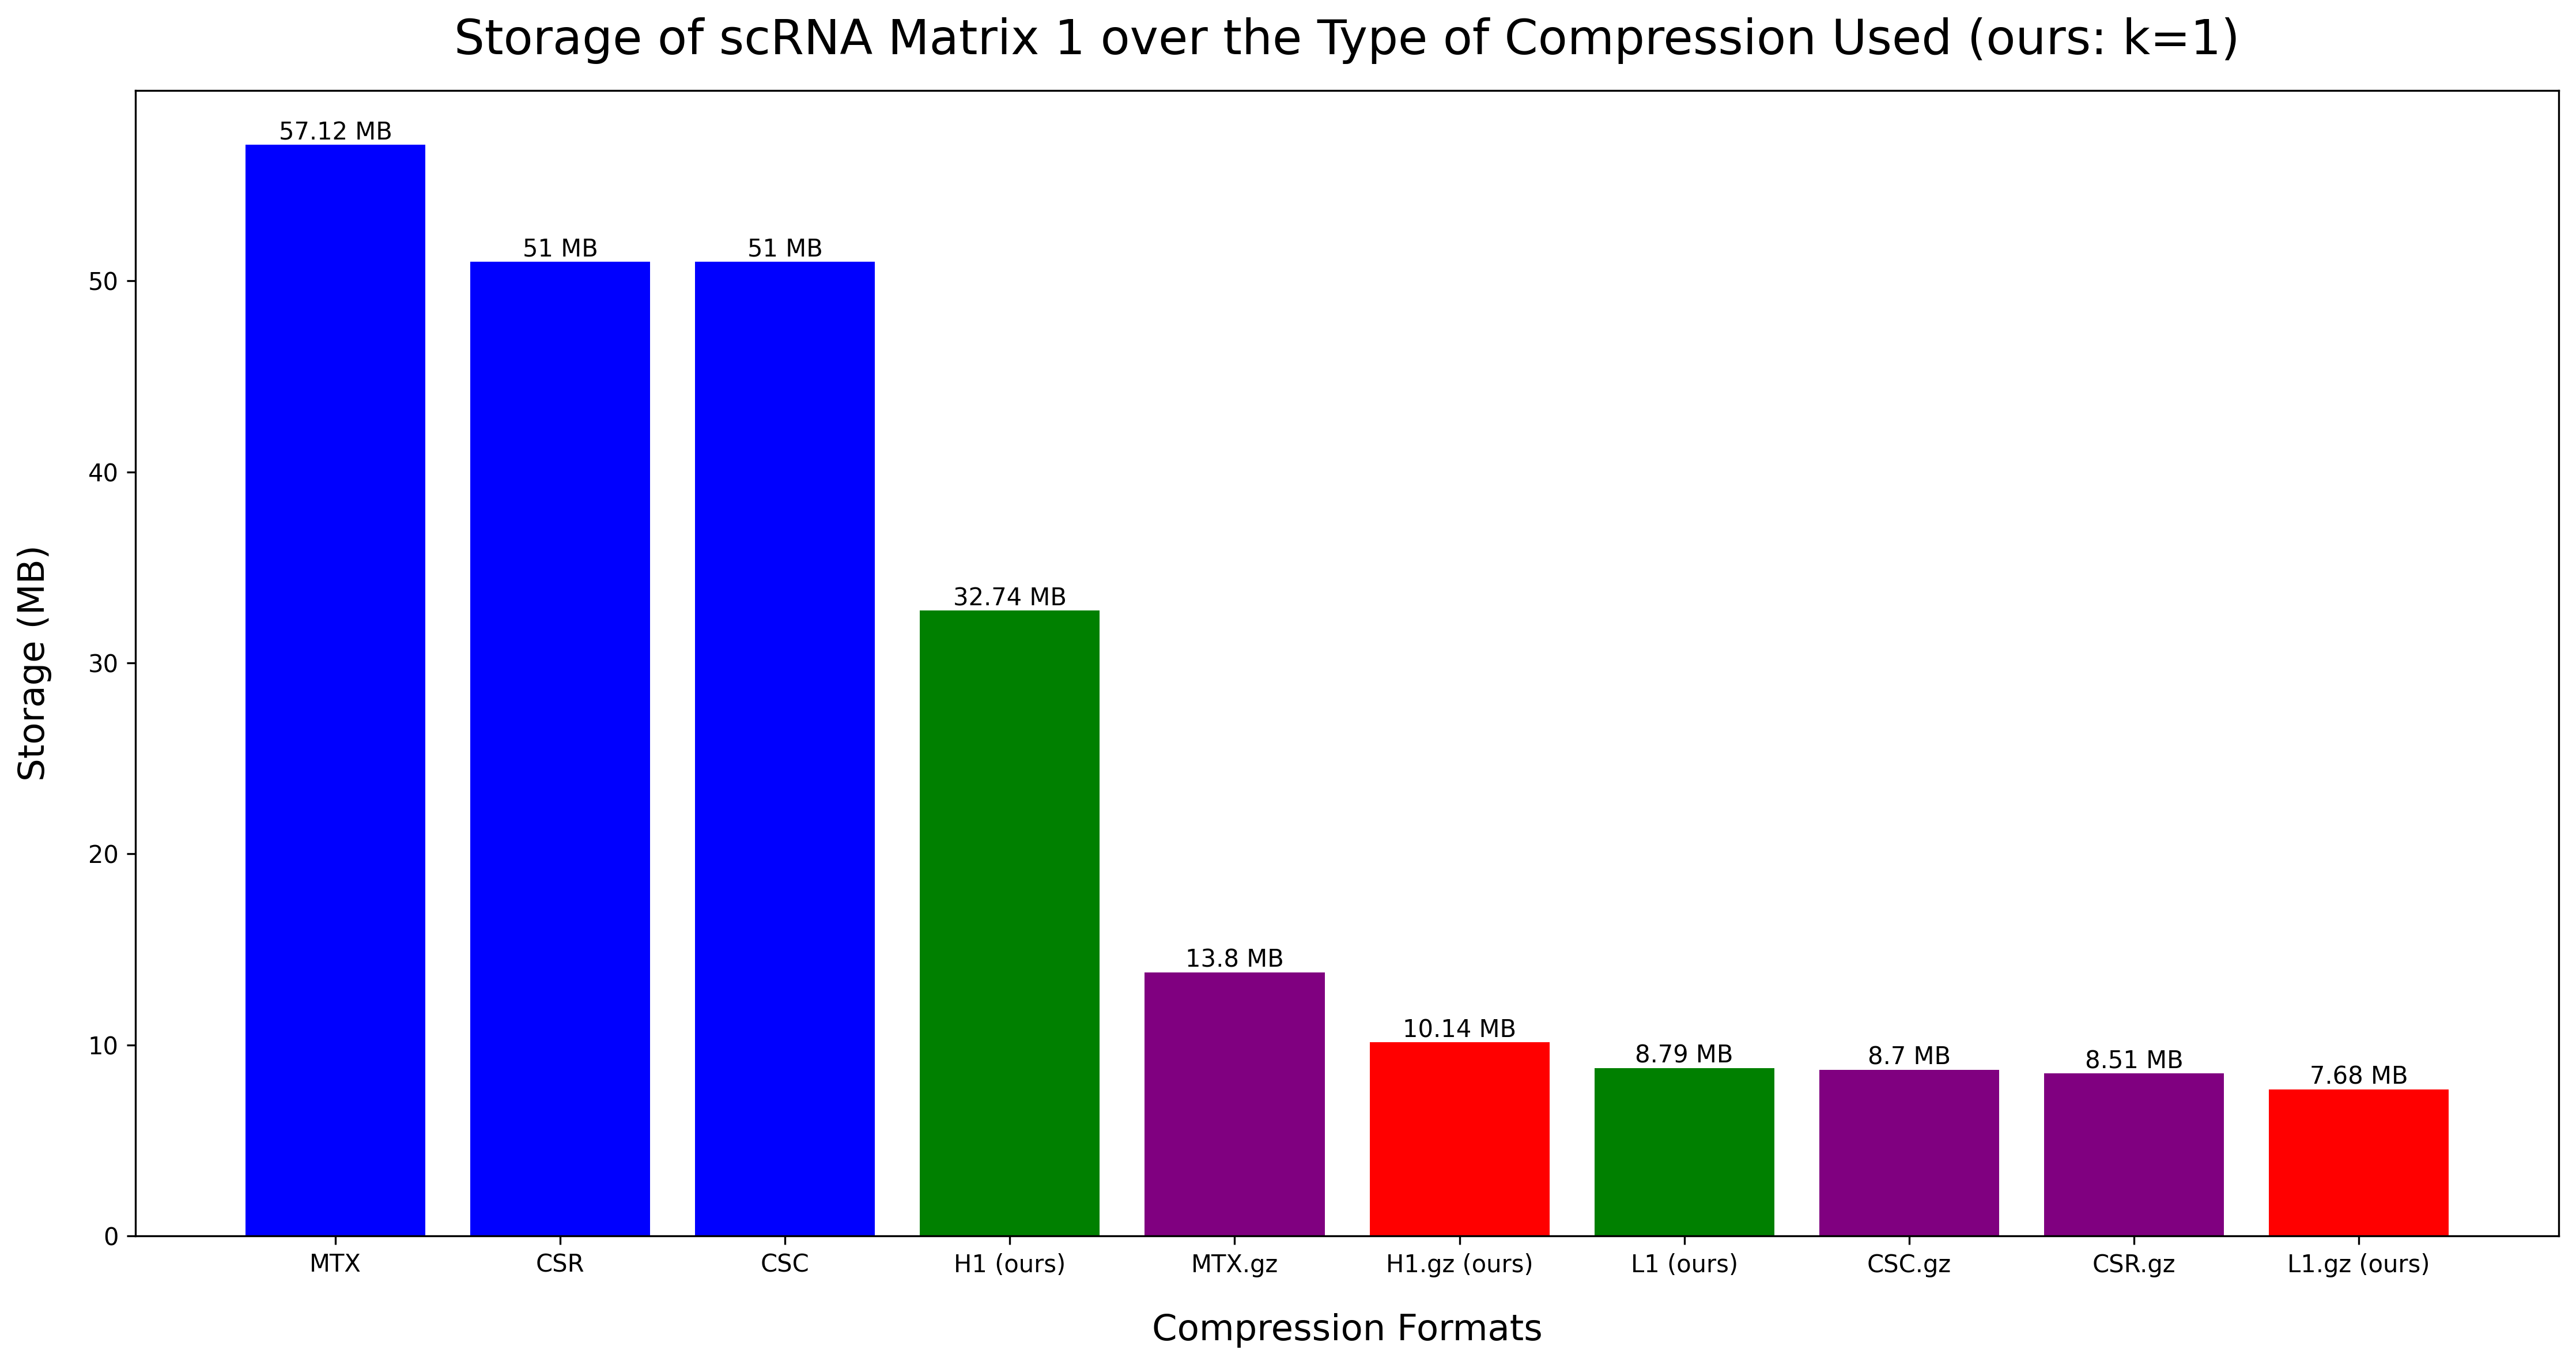
\includegraphics[width=0.35\textwidth]{compressed/kmeans/sample1/k1/storage_comparisons.png}\\
\textit{Comparison of storage sizes for different compression schemes on Sample 1 using $k$-means clustering with $k=1$.}

\textbf{Figure S2. Sample 1, $k$-means, $k=2$}:
\newline
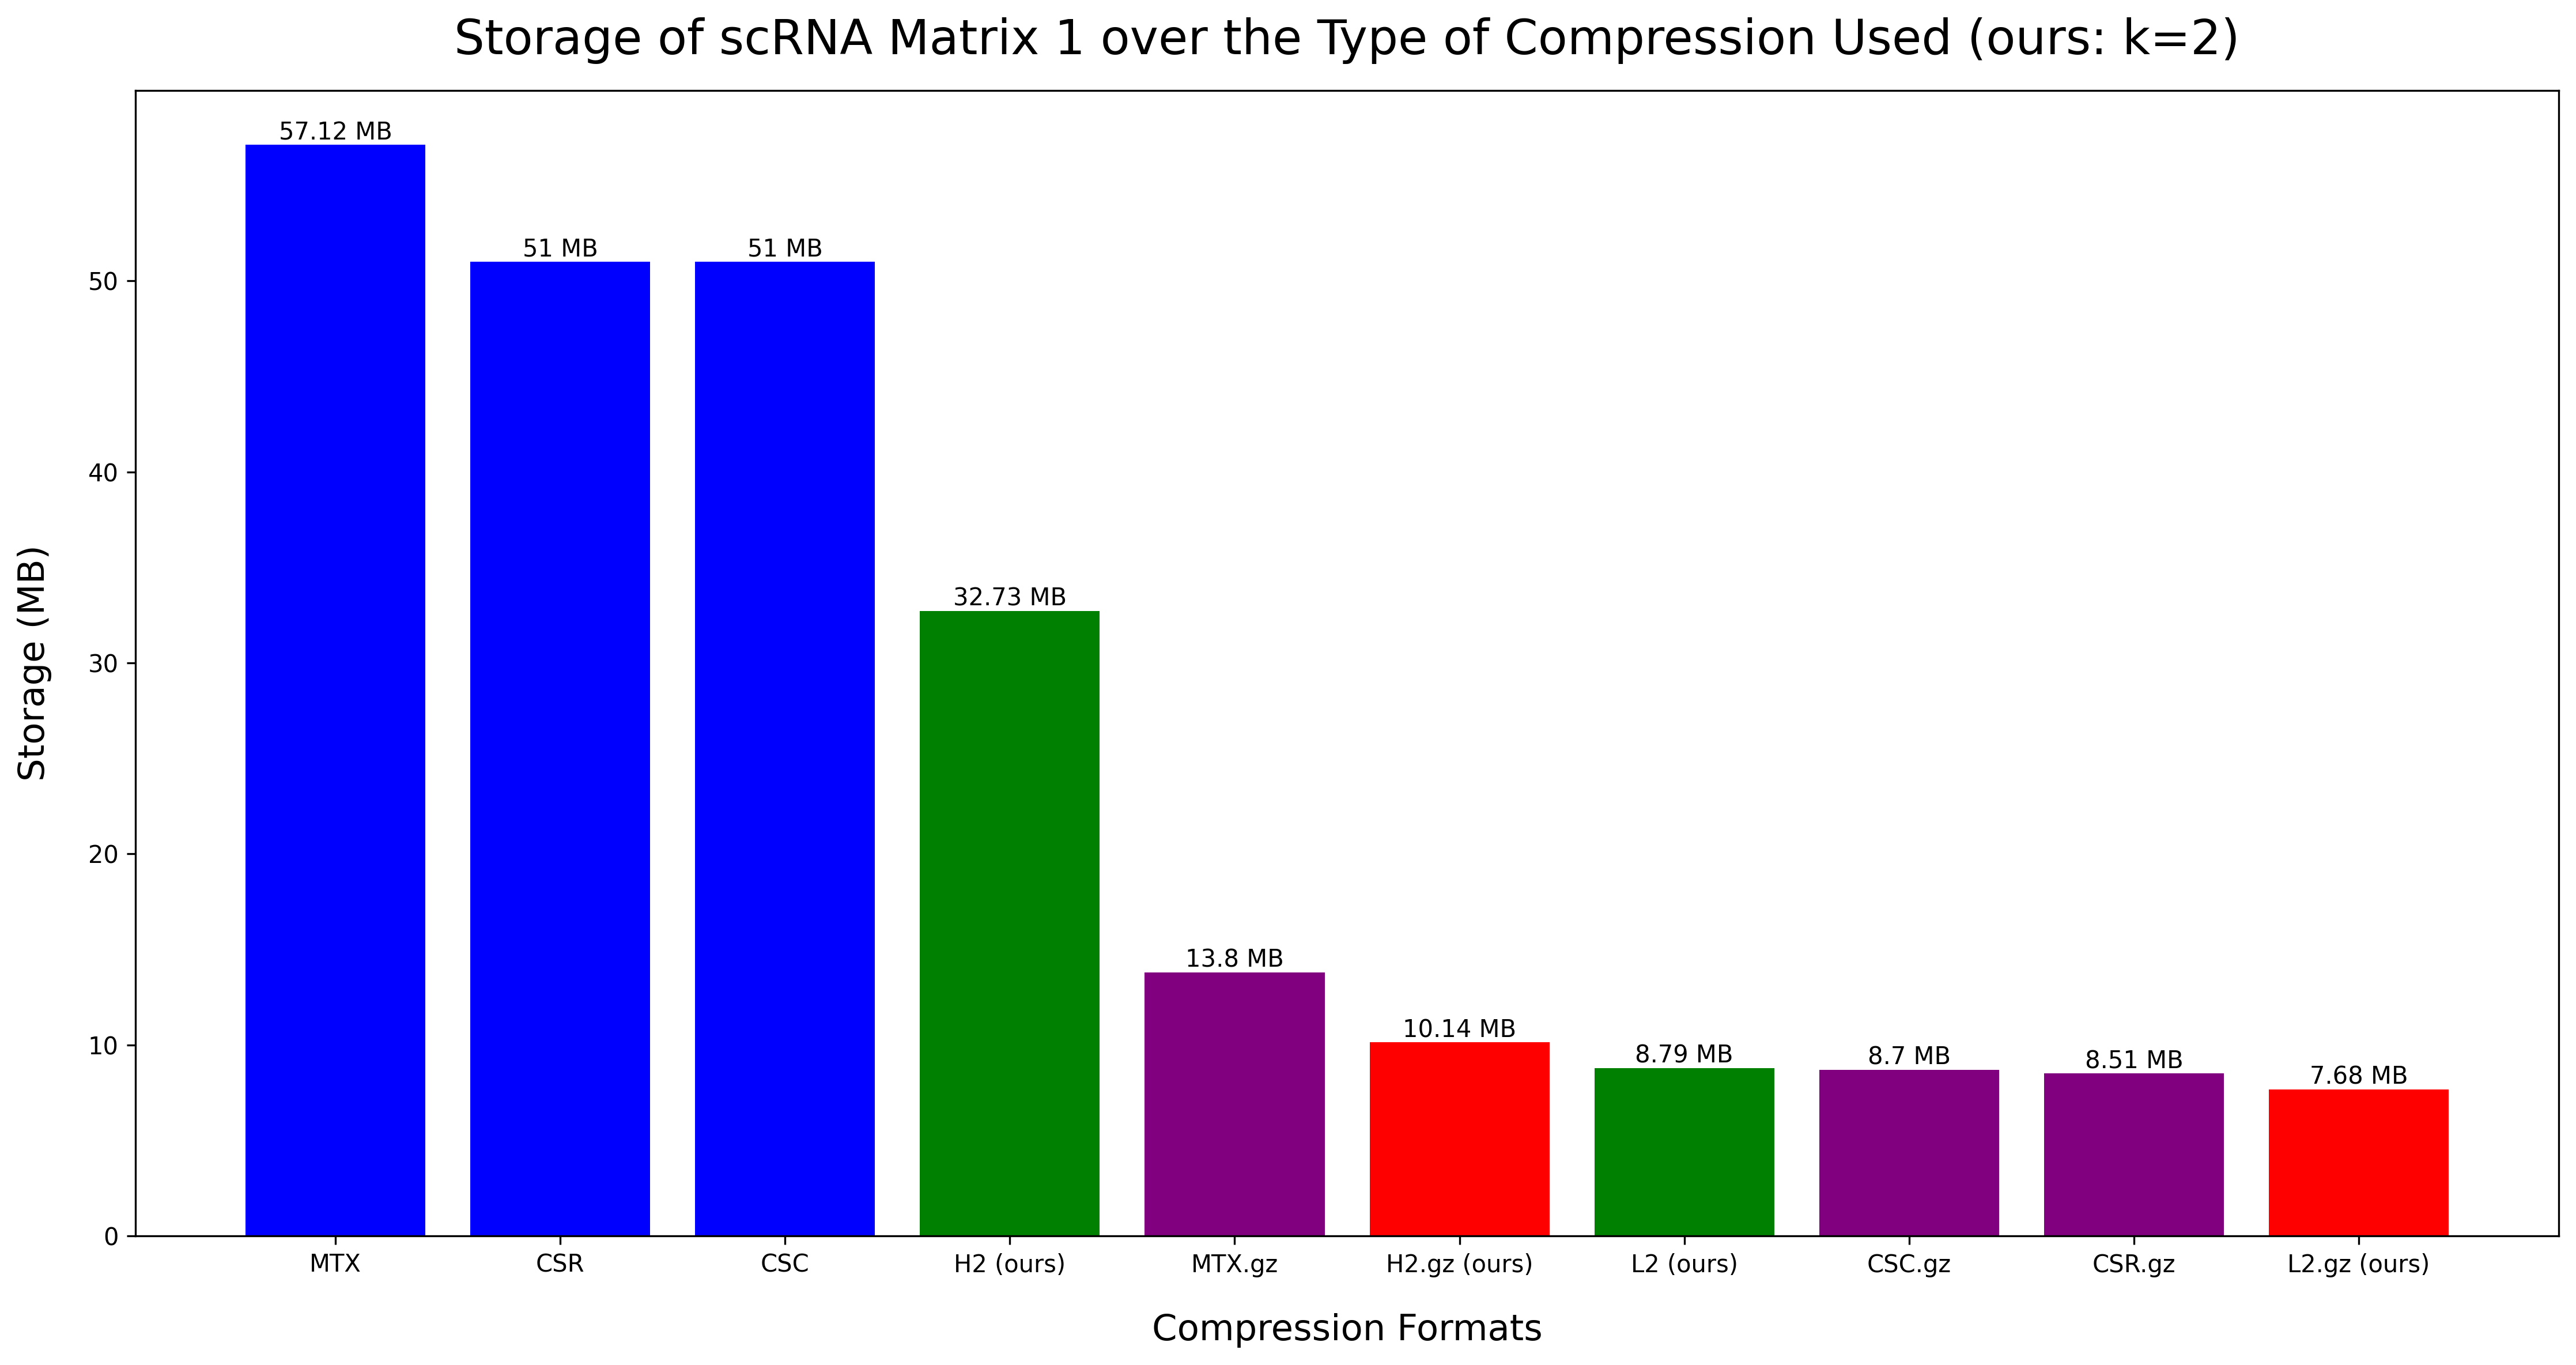
\includegraphics[width=0.35\textwidth]{compressed/kmeans/sample1/k2/storage_comparisons.png}\\
\textit{Comparison of storage sizes for different compression schemes on Sample 1 using $k$-means clustering with $k=2$.}

\textbf{Figure S3. Sample 1, $k$-means, $k=5$}:
\newline
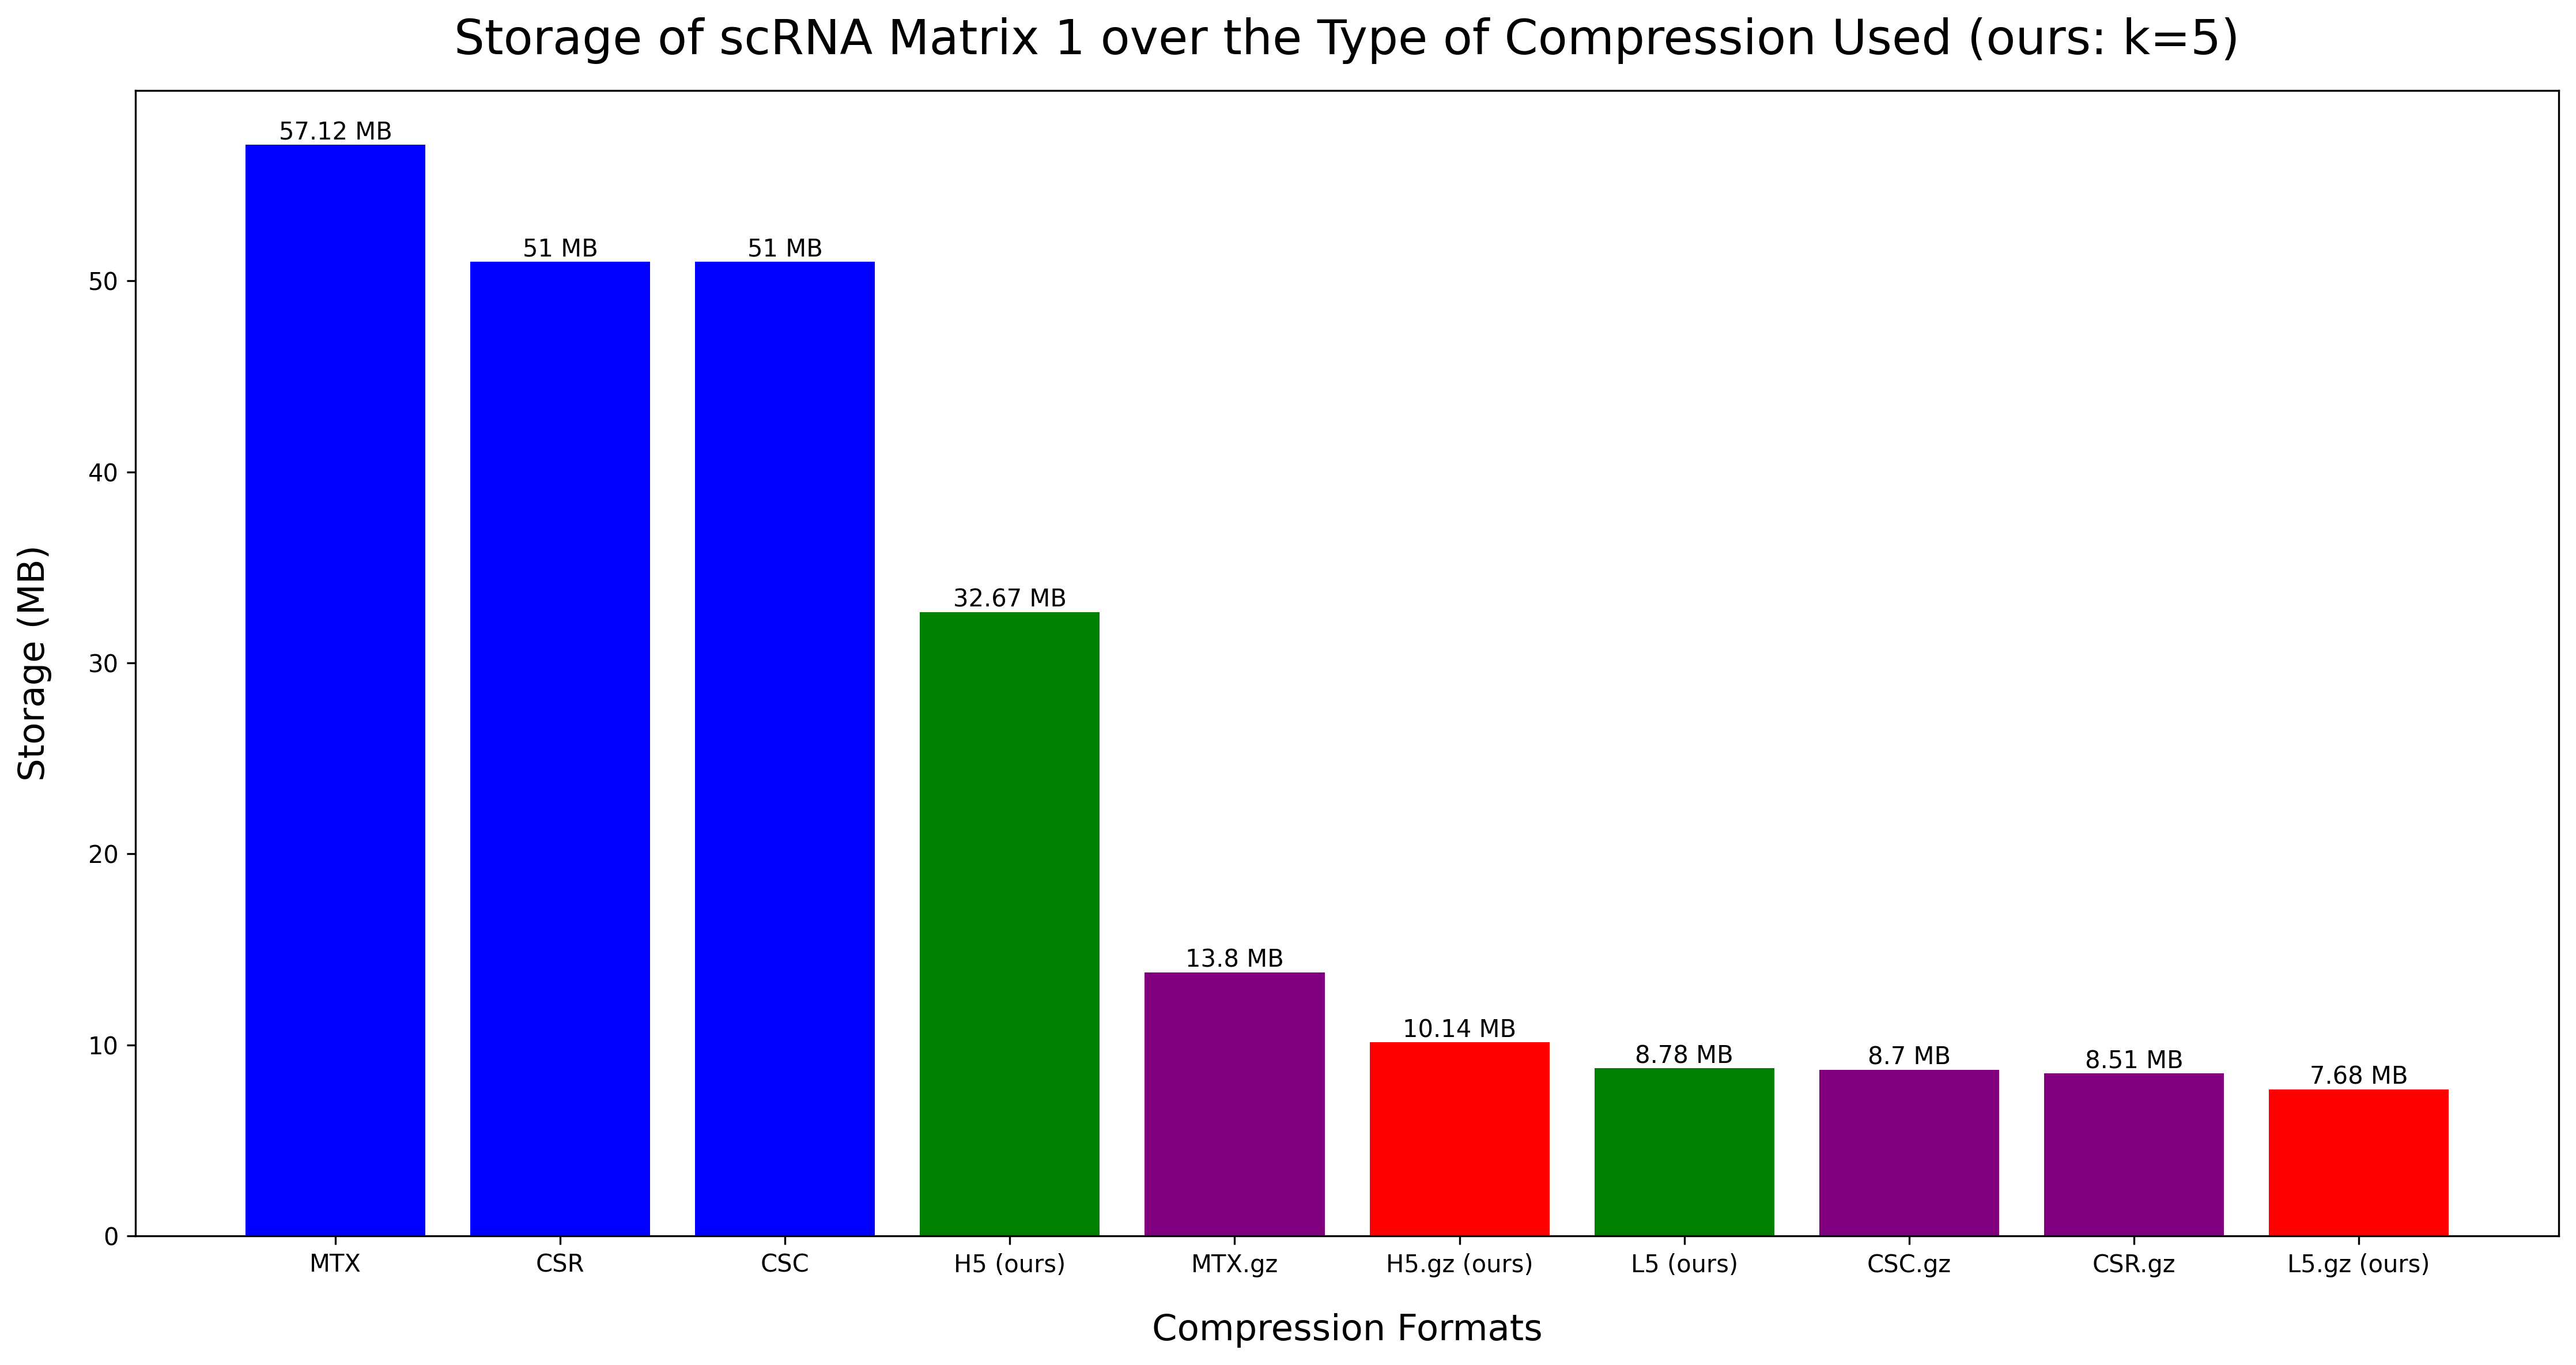
\includegraphics[width=0.35\textwidth]{compressed/kmeans/sample1/k5/storage_comparisons.png}\\
\textit{Comparison of storage sizes for different compression schemes on Sample 1 using $k$-means clustering with $k=5$.}

\textbf{Figure S4. Sample 1, $k$-means, $k=10$}:
\newline
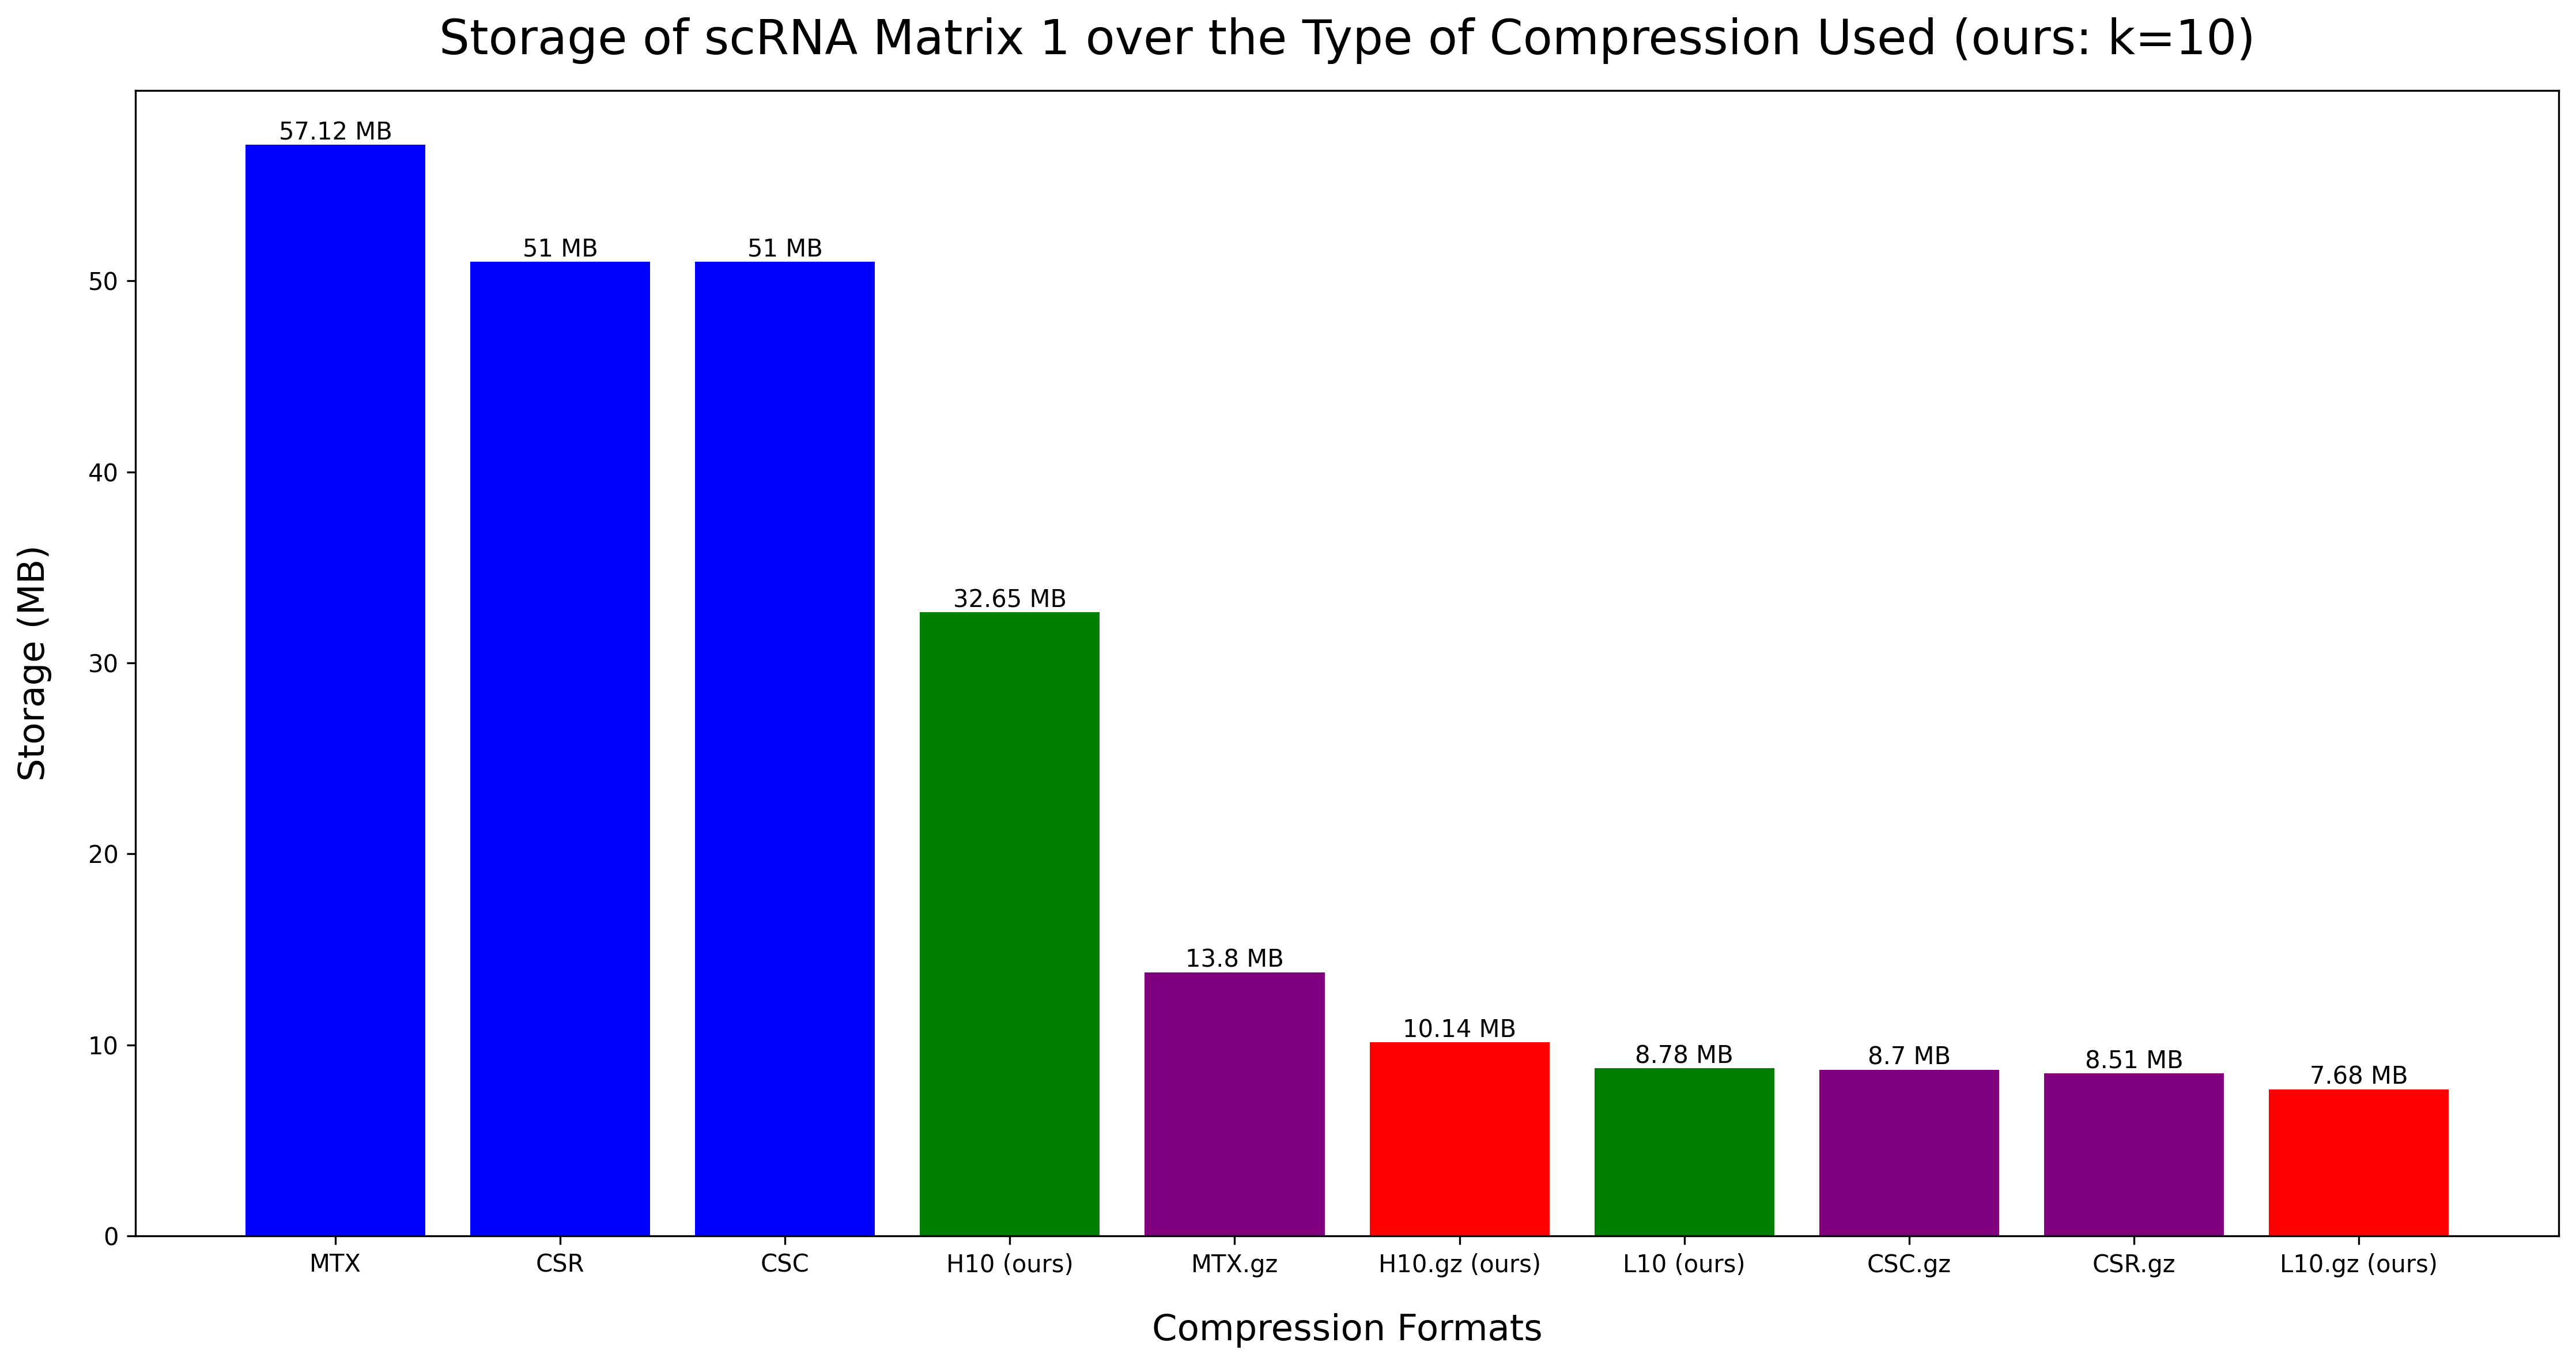
\includegraphics[width=0.35\textwidth]{compressed/kmeans/sample1/k10/storage_comparisons.png}\\
\textit{Comparison of storage sizes for different compression schemes on Sample 1 using $k$-means clustering with $k=10$.}

\textbf{Figure S5. Sample 1, $k$-means, $k=20$}:
\newline
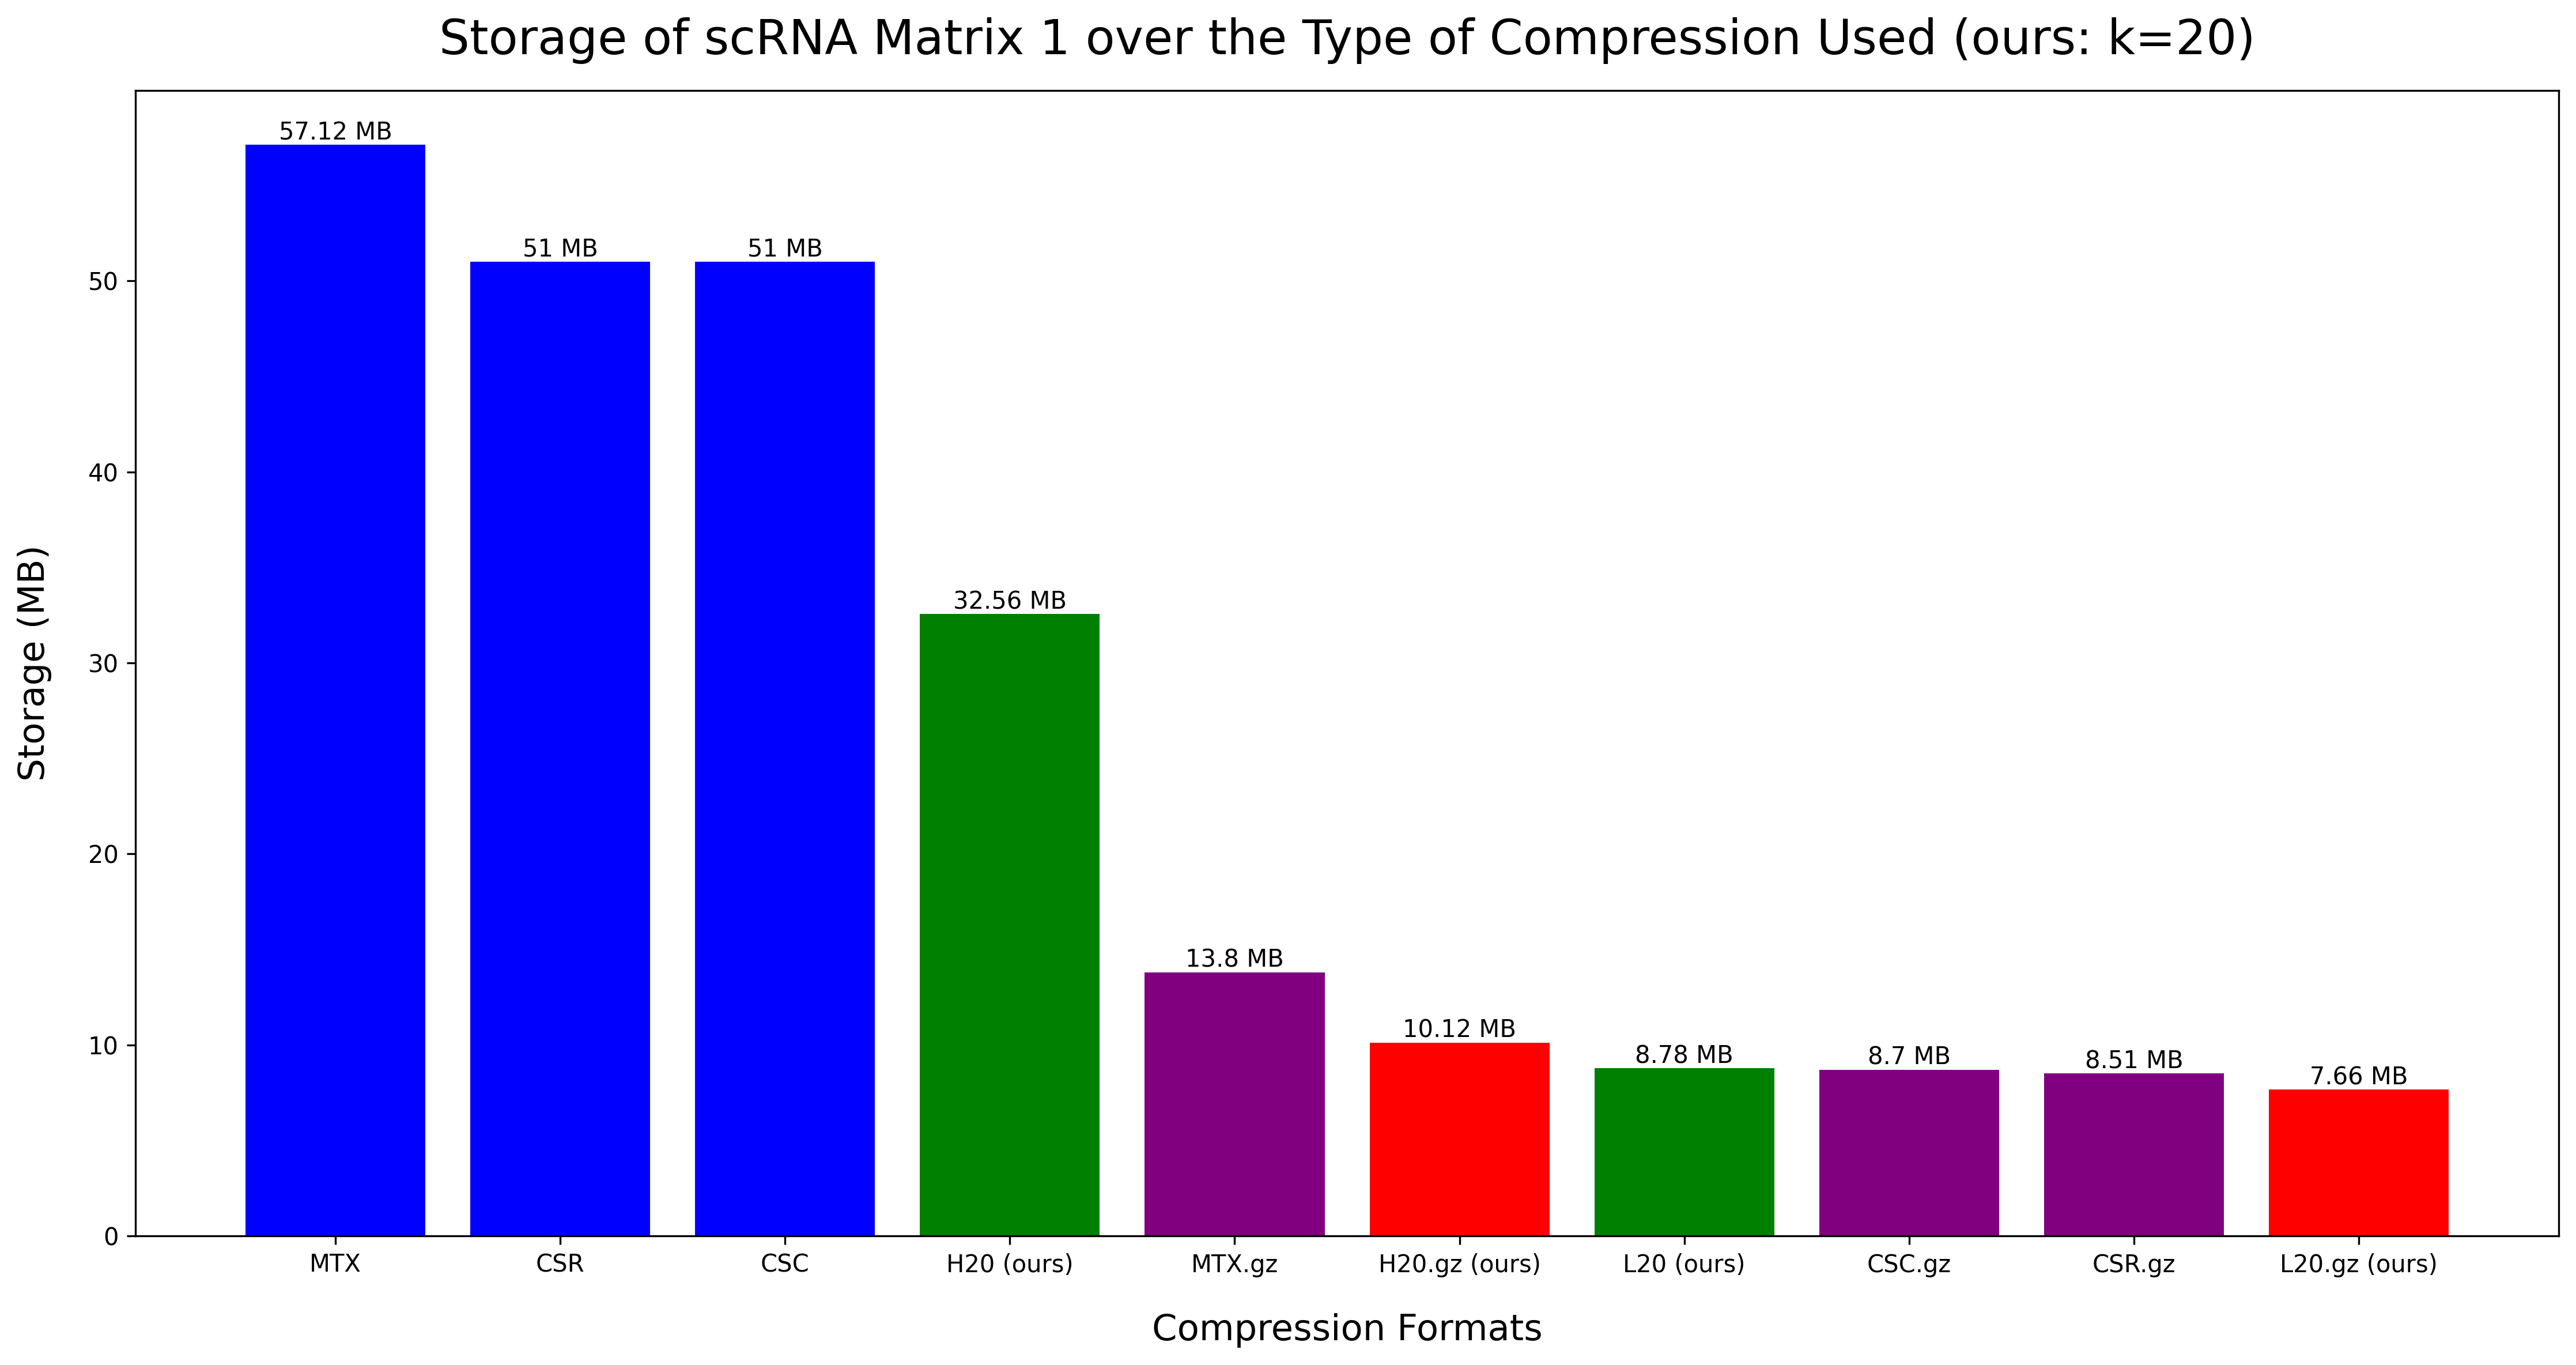
\includegraphics[width=0.35\textwidth]{compressed/kmeans/sample1/k20/storage_comparisons.png}\\
\textit{Comparison of storage sizes for different compression schemes on Sample 1 using $k$-means clustering with $k=20$.}

\textbf{Figure S6. Sample 1, $k$-means, $k=30$}:
\newline
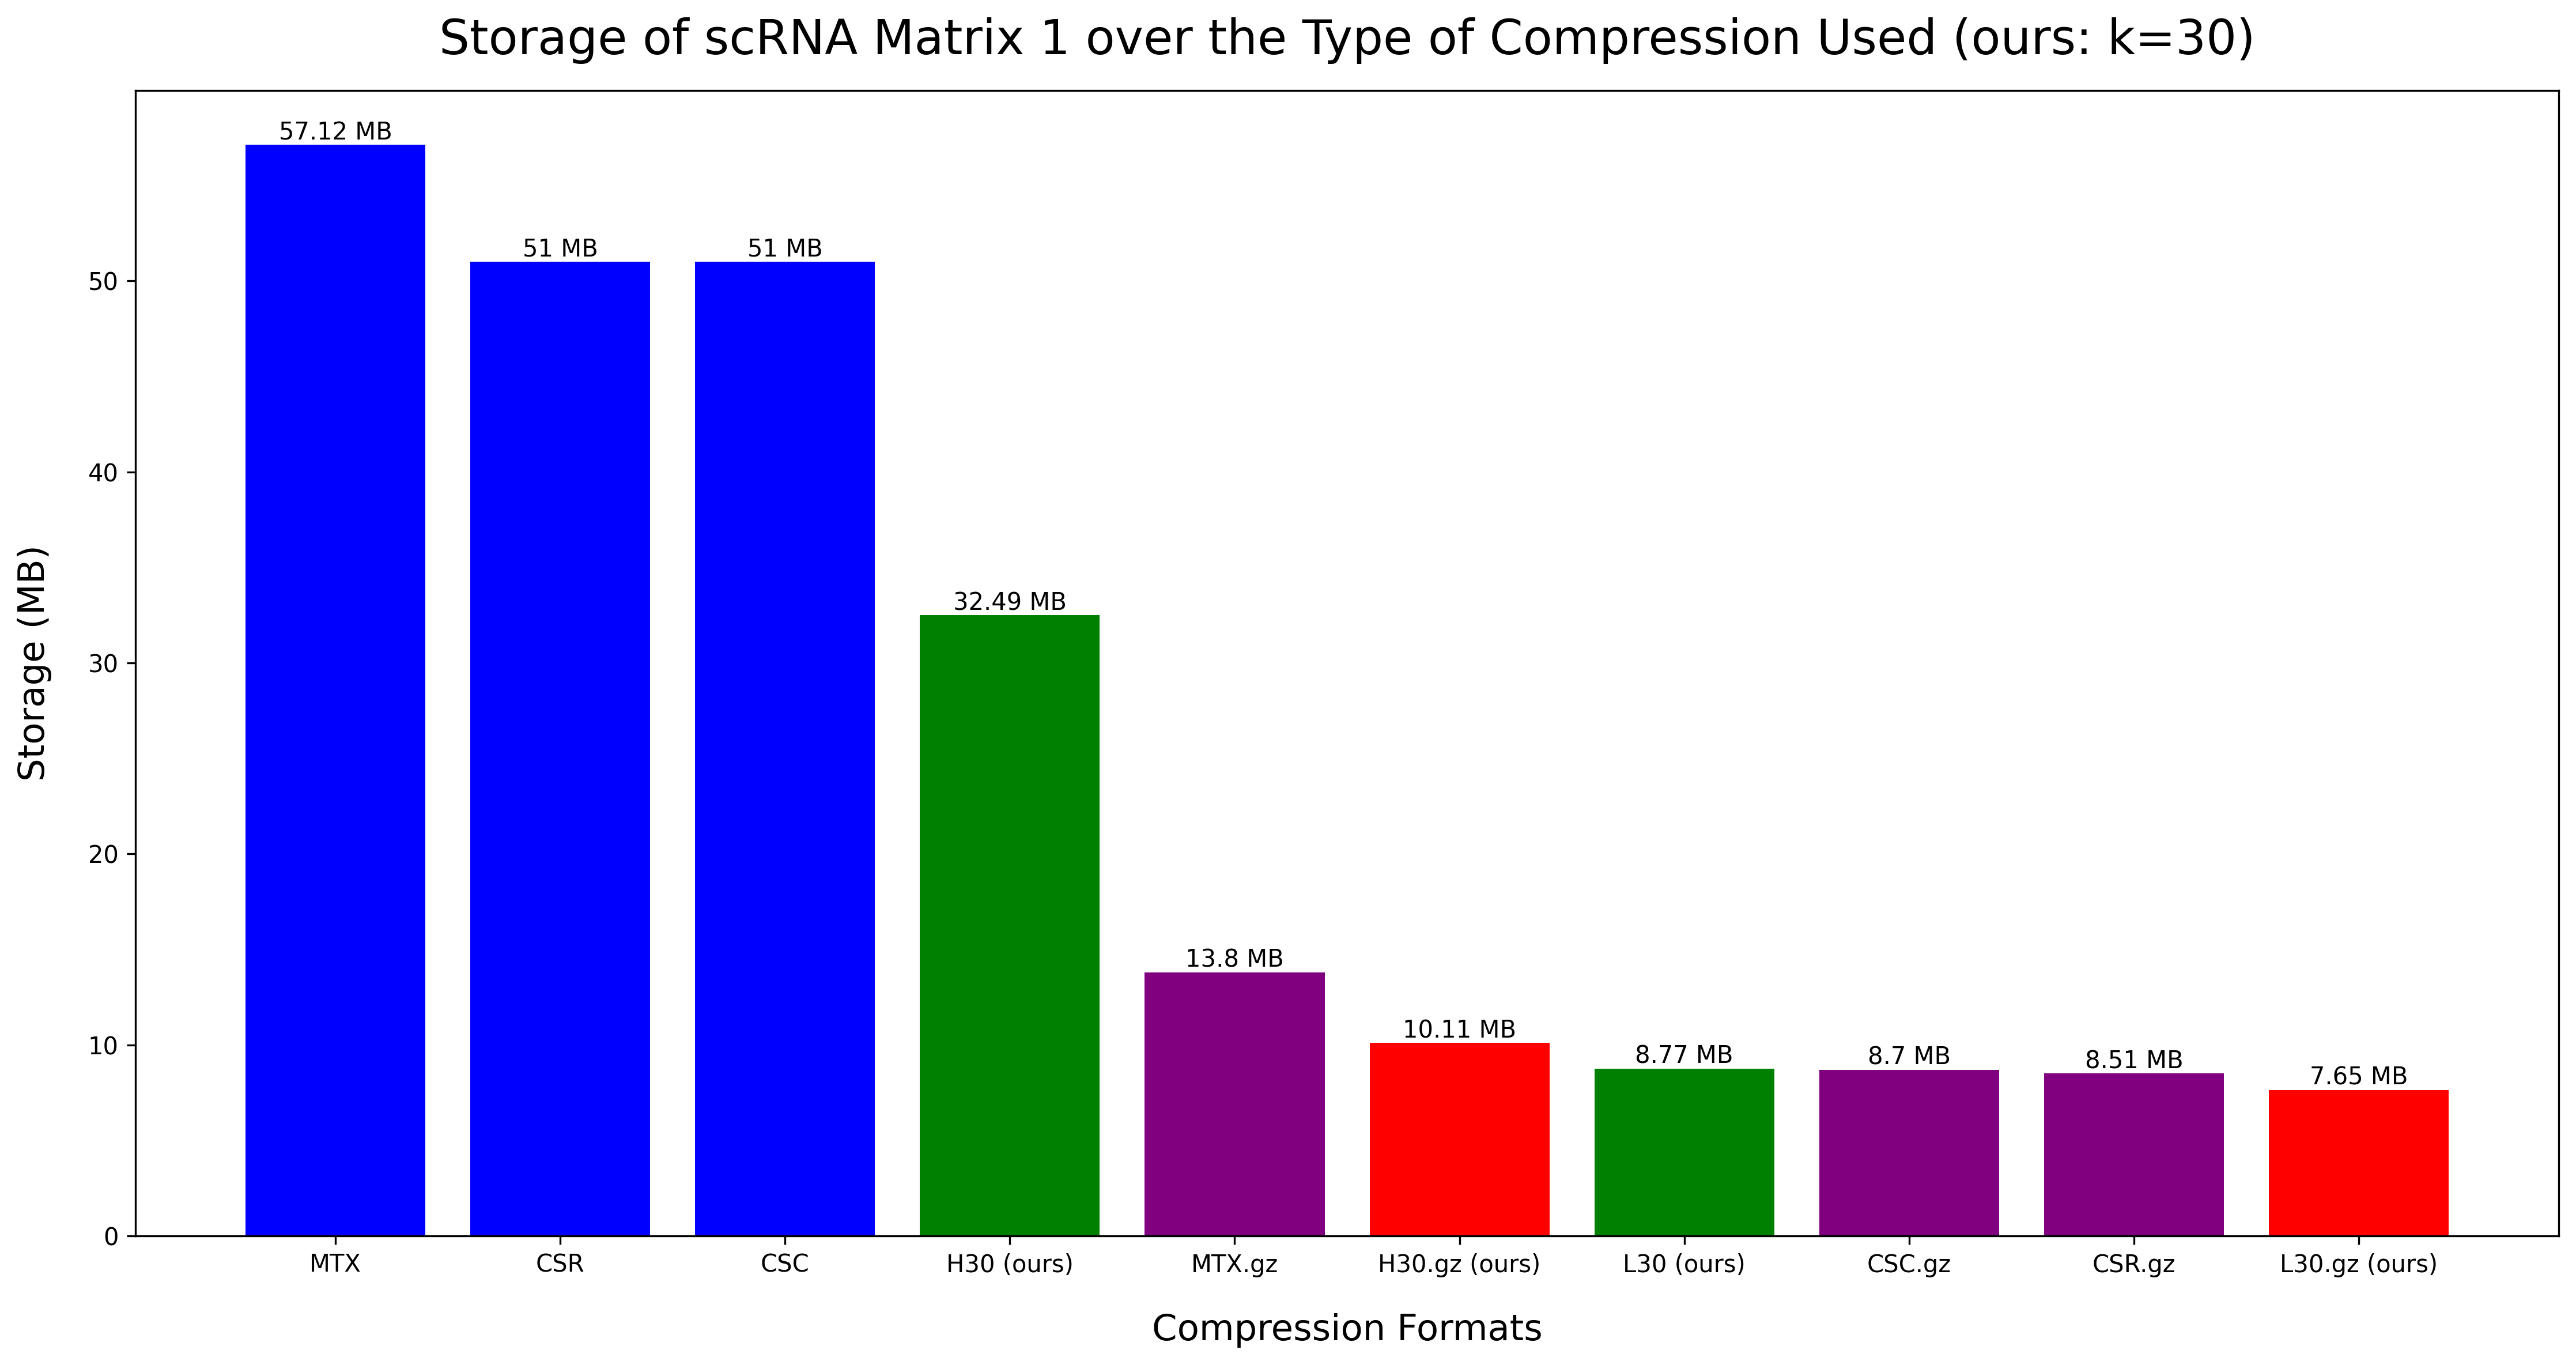
\includegraphics[width=0.35\textwidth]{compressed/kmeans/sample1/k30/storage_comparisons.png}\\
\textit{Comparison of storage sizes for different compression schemes on Sample 1 using $k$-means clustering with $k=30$.}

\textbf{Figure S7. Sample 2, $k$-means, $k=1$}:
\newline
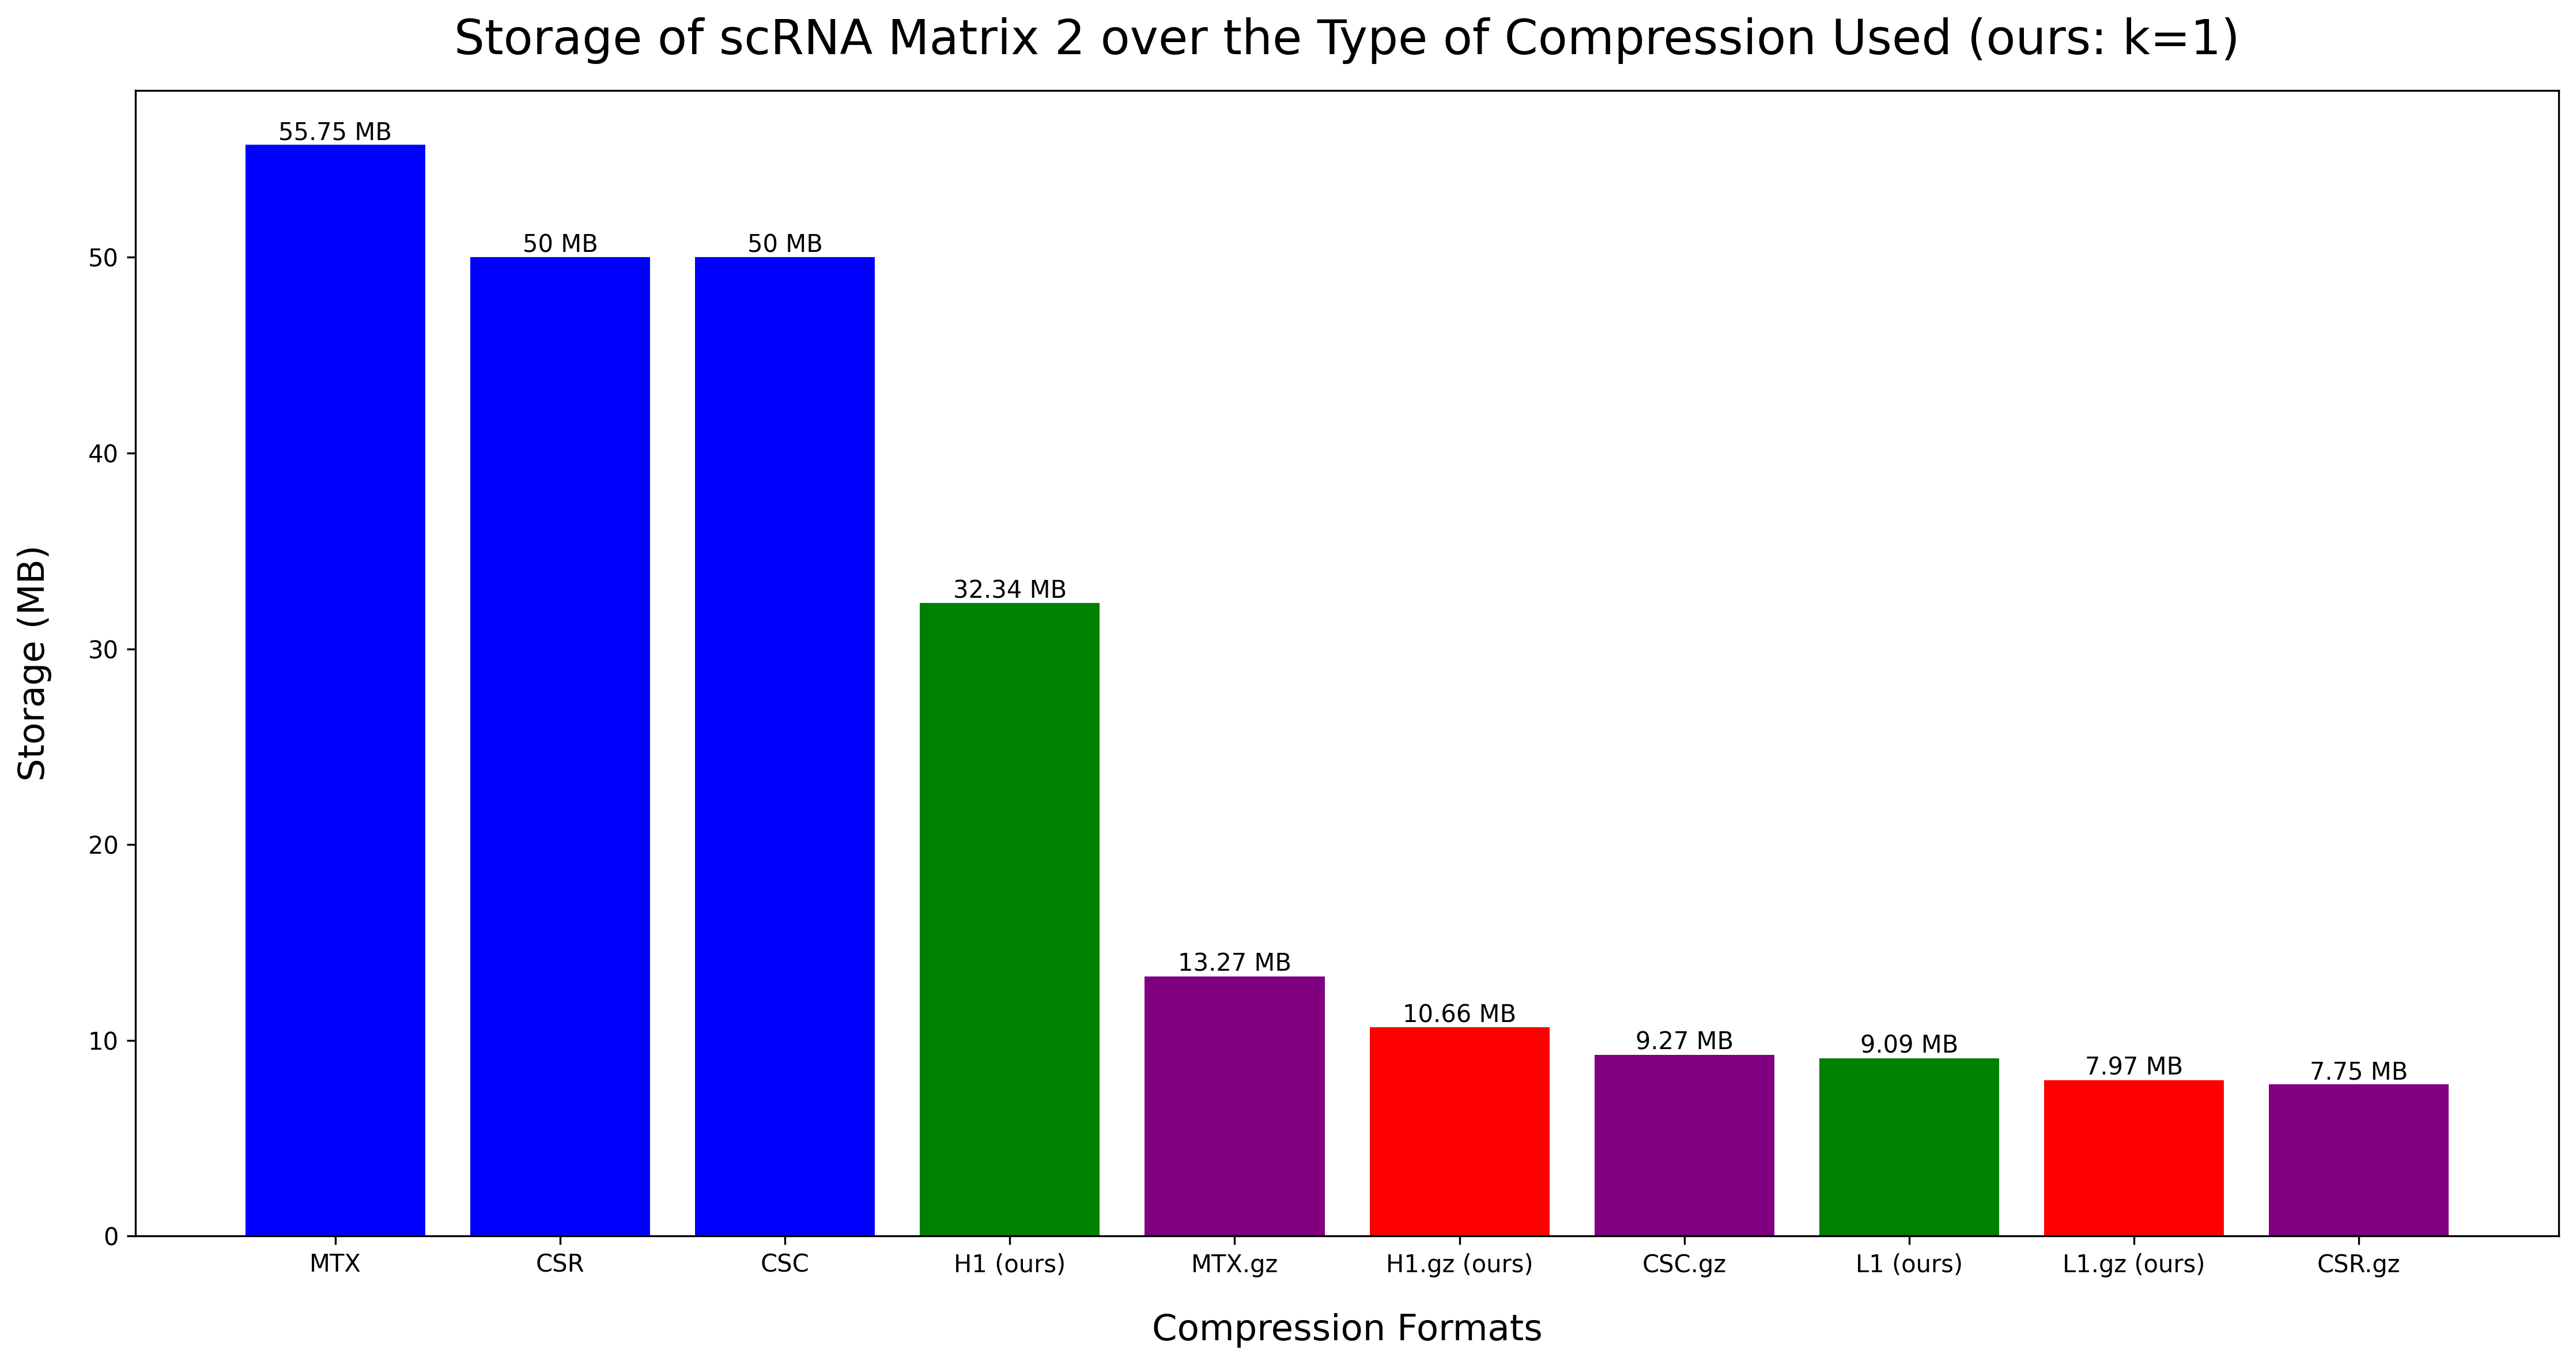
\includegraphics[width=0.35\textwidth]{compressed/kmeans/sample2/k1/storage_comparisons.png}\\
\textit{Comparison of storage sizes for different compression schemes on Sample 2 using $k$-means clustering with $k=1$.}

\textbf{Figure S8. Sample 2, $k$-means, $k=2$}:
\newline
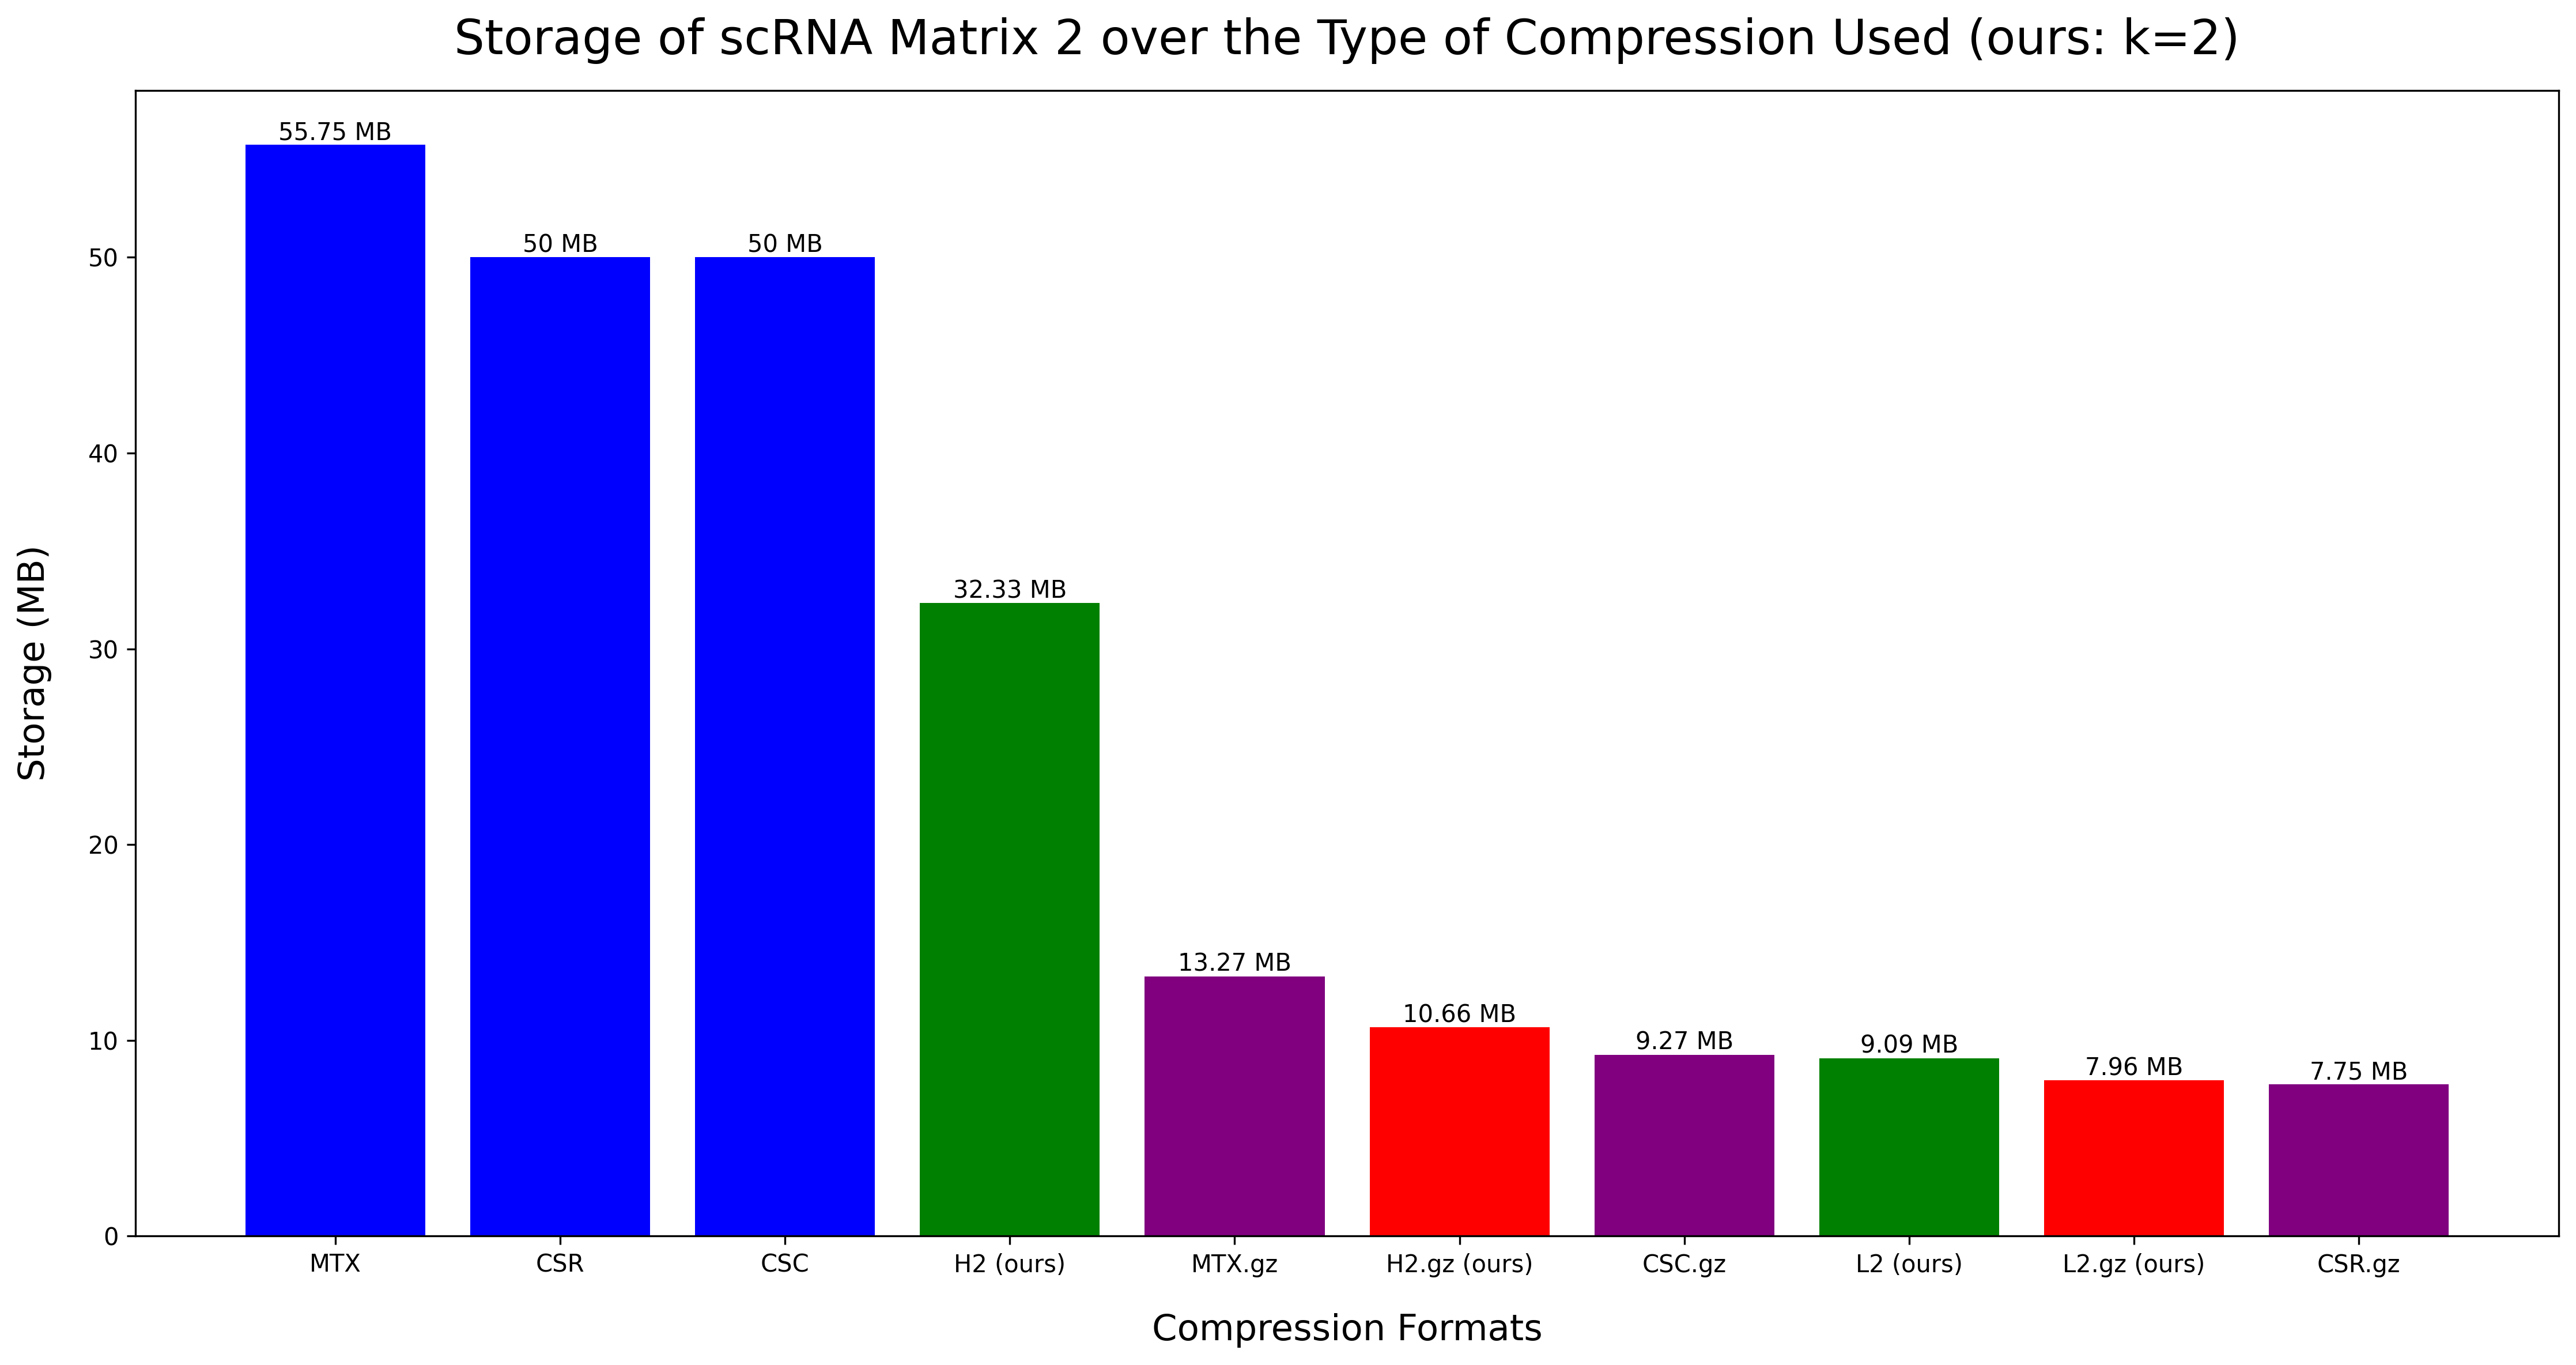
\includegraphics[width=0.35\textwidth]{compressed/kmeans/sample2/k2/storage_comparisons.png}\\
\textit{Comparison of storage sizes for different compression schemes on Sample 2 using $k$-means clustering with $k=2$.}

\textbf{Figure S9. Sample 2, $k$-means, $k=5$}:
\newline
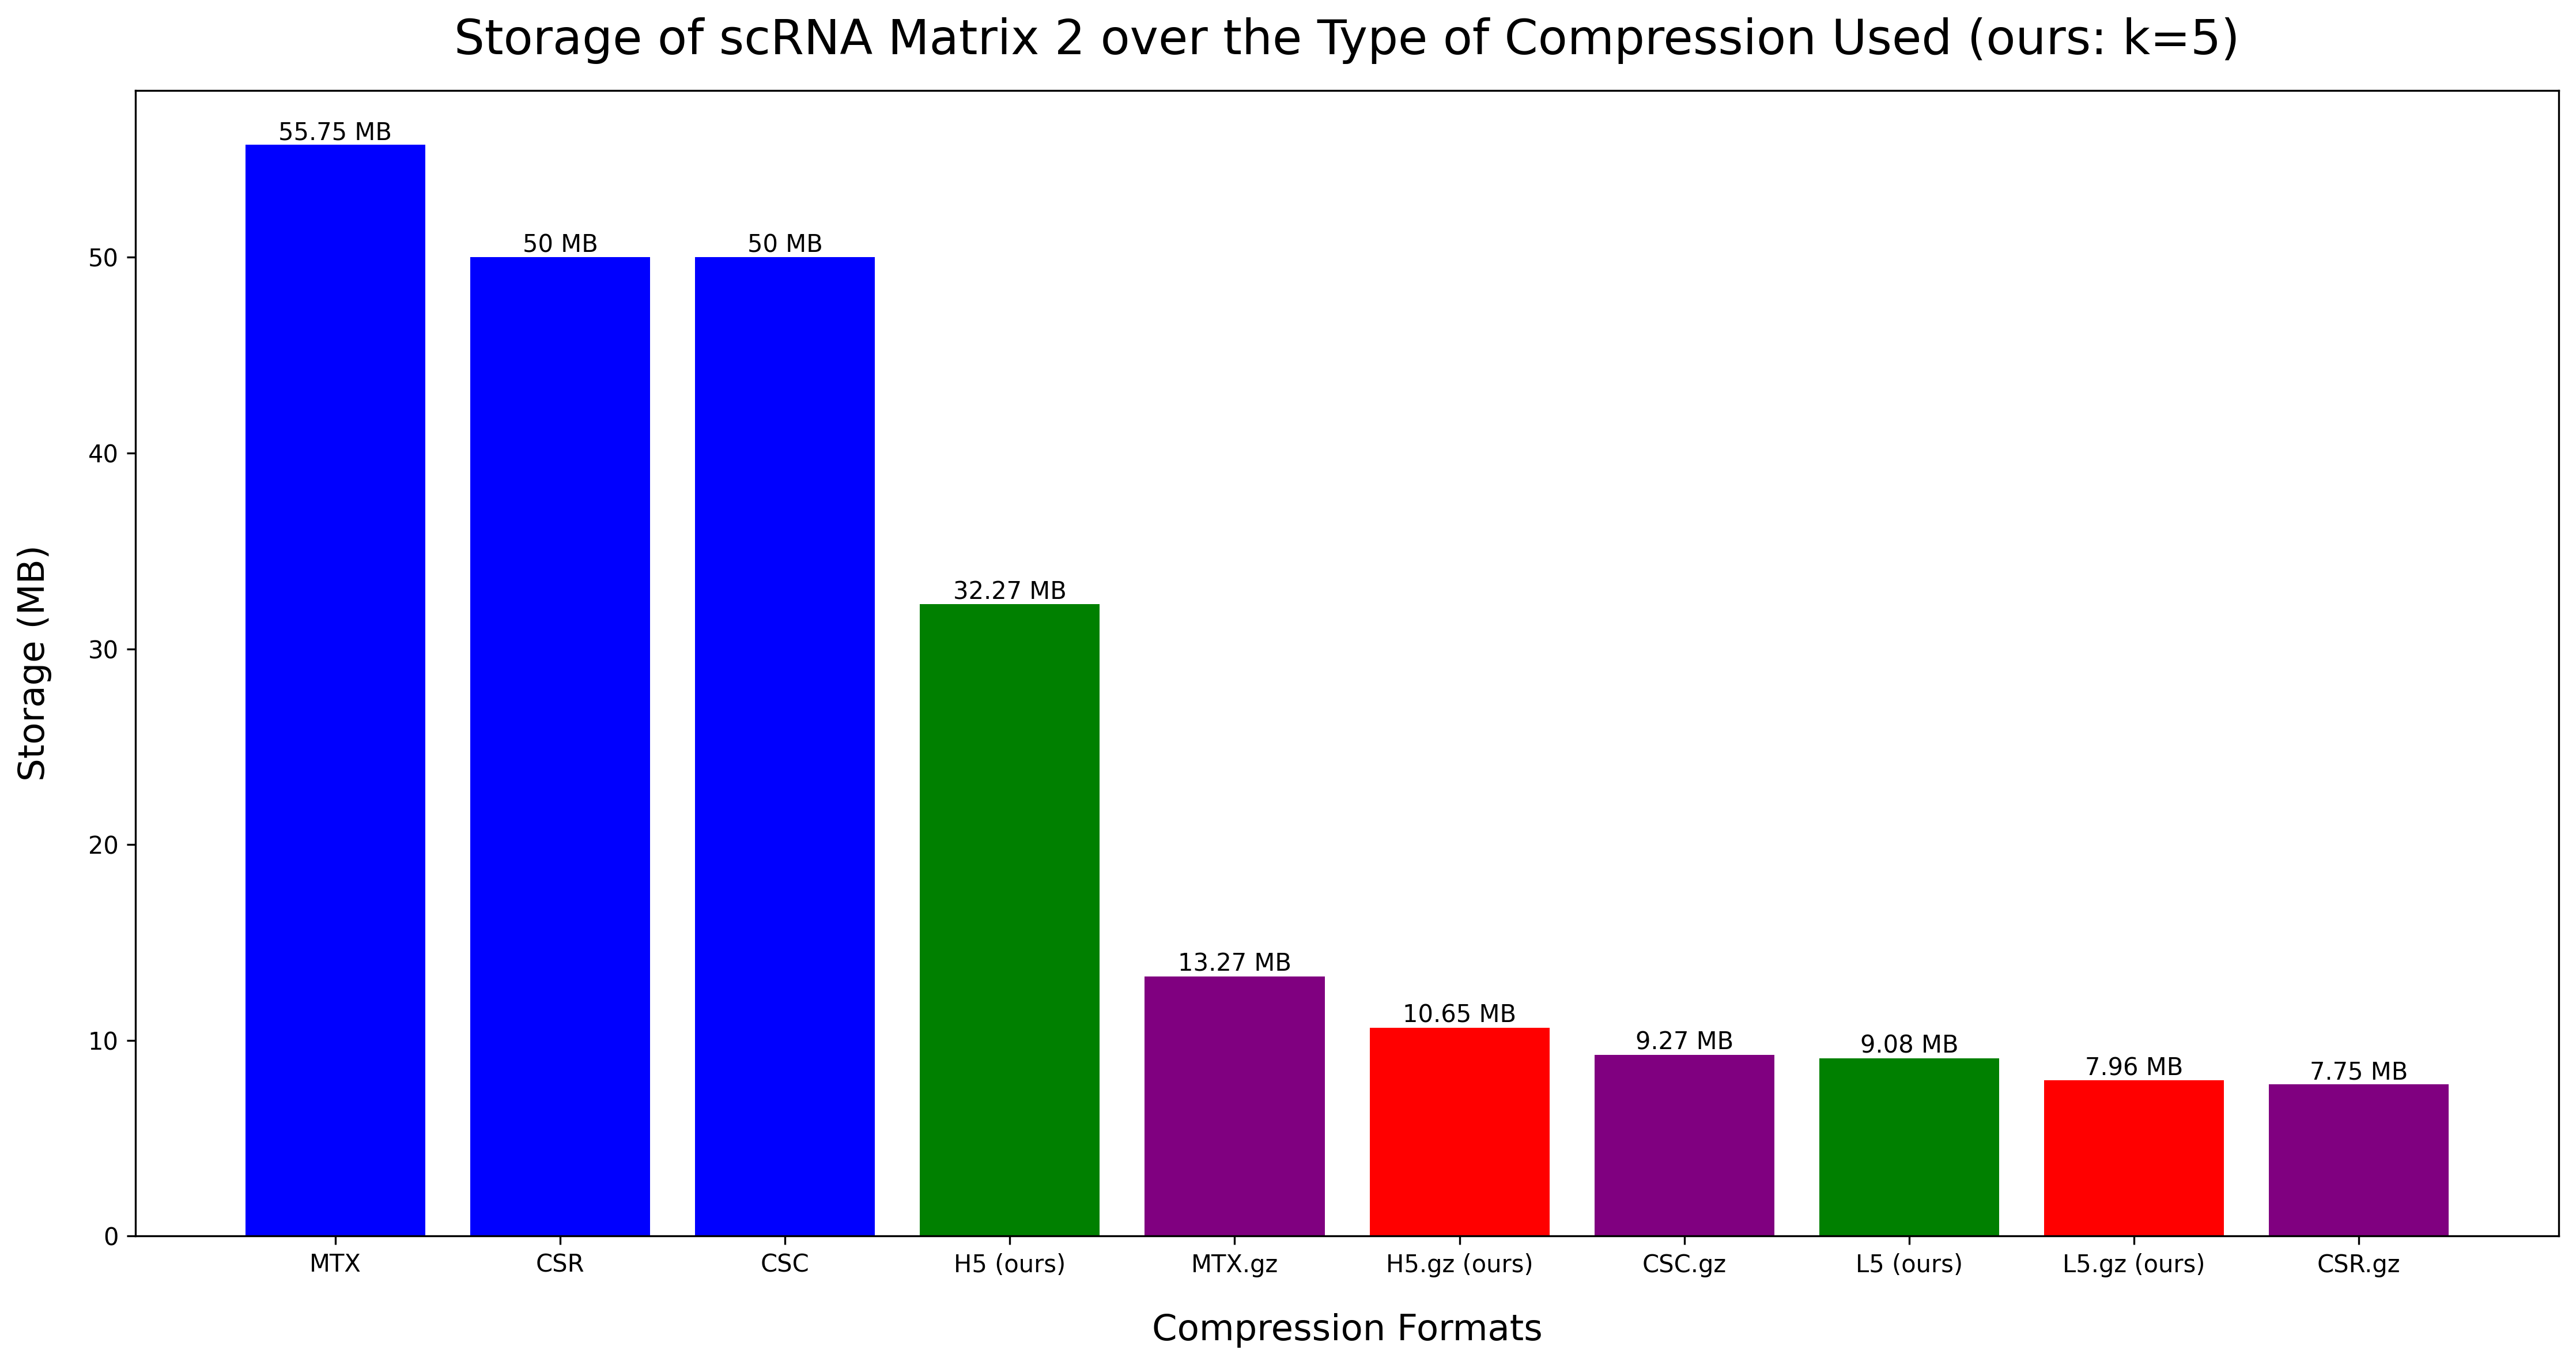
\includegraphics[width=0.35\textwidth]{compressed/kmeans/sample2/k5/storage_comparisons.png}\\
\textit{Comparison of storage sizes for different compression schemes on Sample 2 using $k$-means clustering with $k=5$.}

\textbf{Figure S10. Sample 2, $k$-means, $k=10$}:
\newline
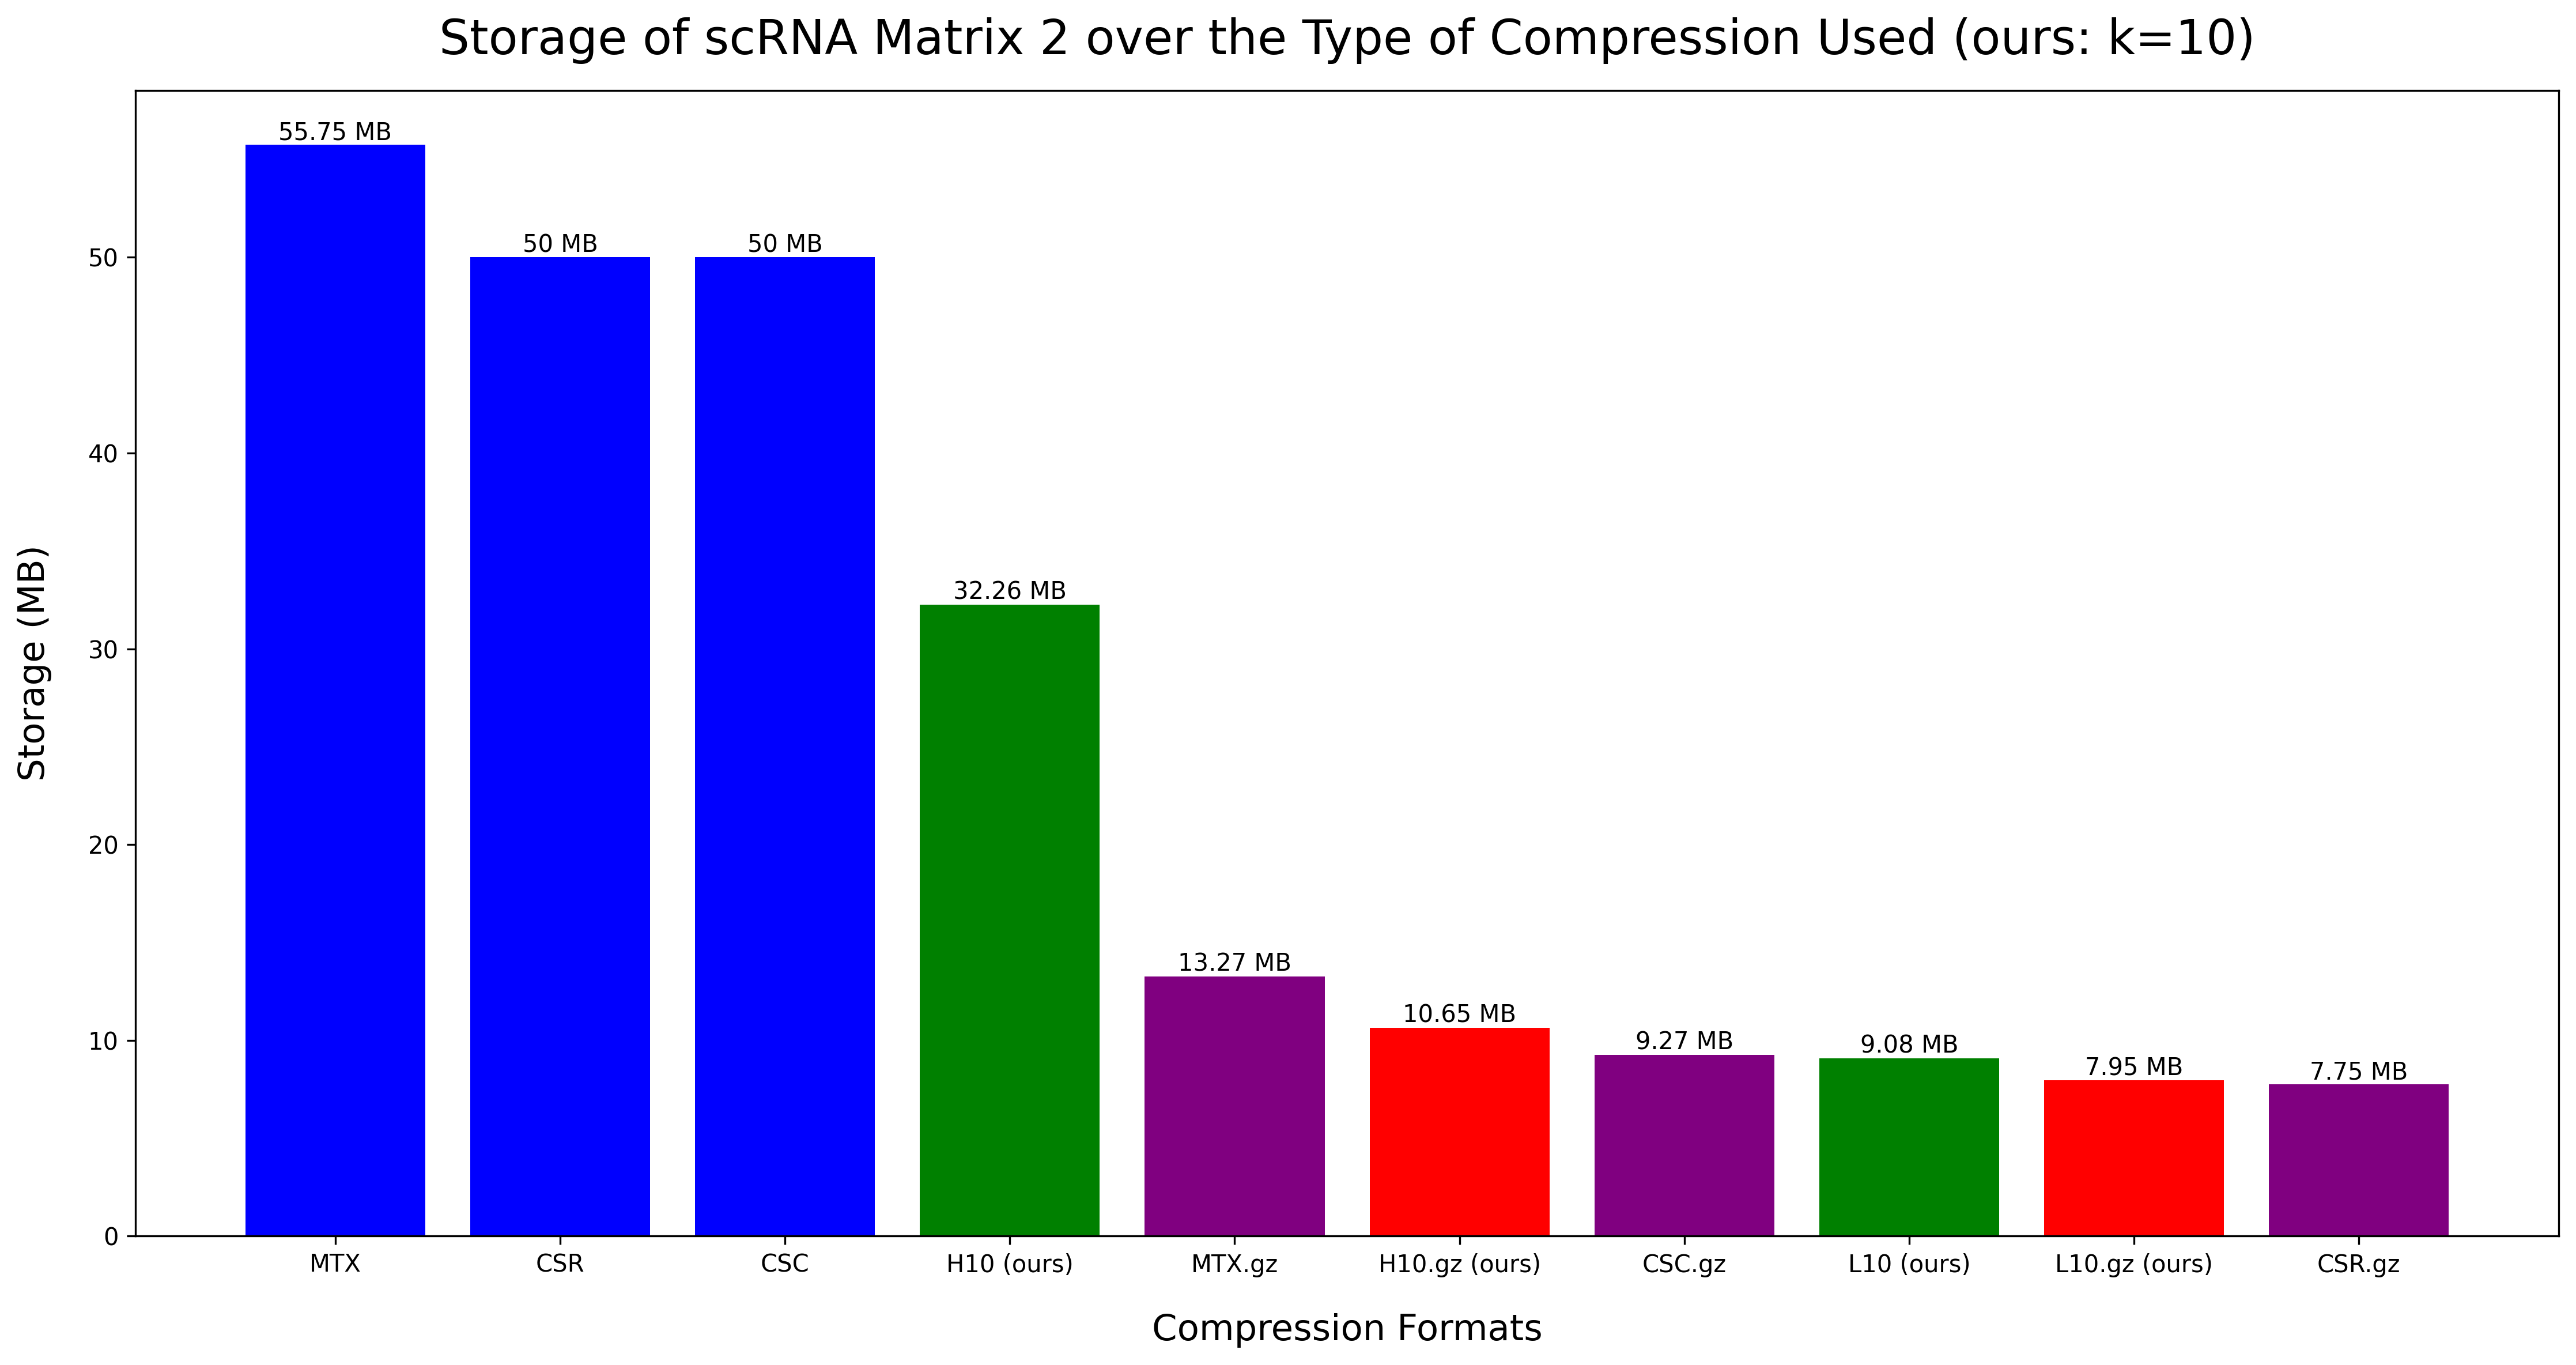
\includegraphics[width=0.35\textwidth]{compressed/kmeans/sample2/k10/storage_comparisons.png}\\
\textit{Comparison of storage sizes for different compression schemes on Sample 2 using $k$-means clustering with $k=10$.}

\textbf{Figure S11. Sample 2, $k$-means, $k=20$}:
\newline
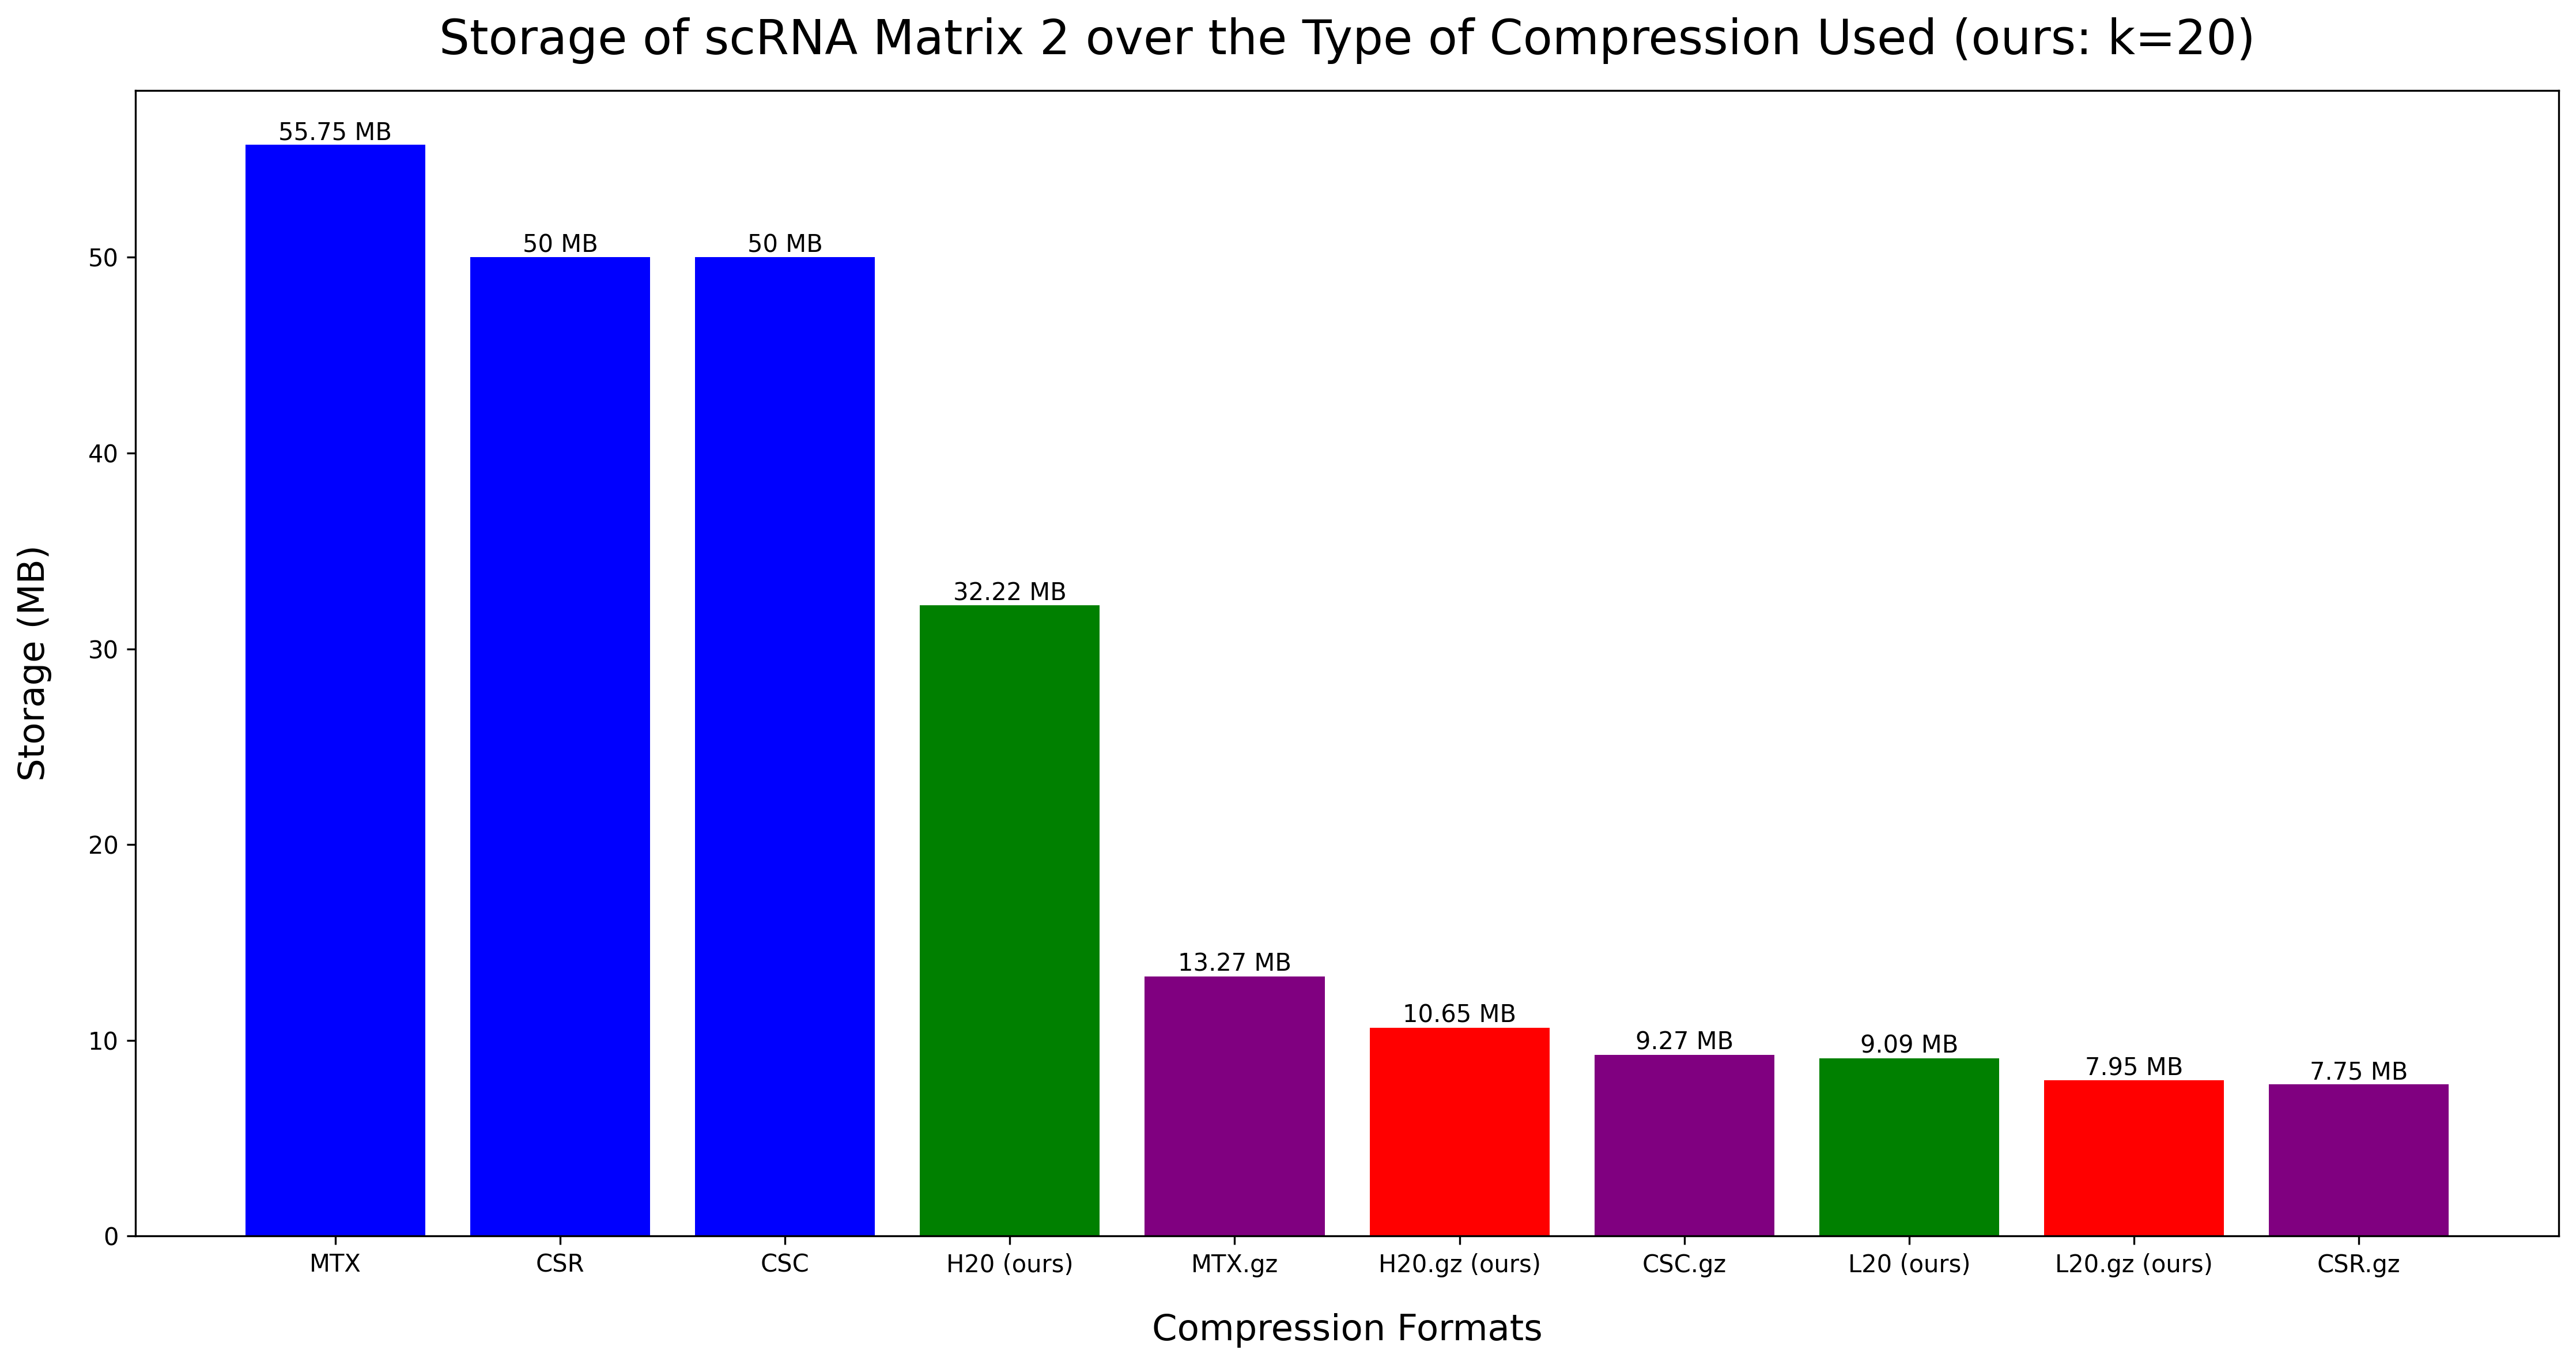
\includegraphics[width=0.35\textwidth]{compressed/kmeans/sample2/k20/storage_comparisons.png}\\
\textit{Comparison of storage sizes for different compression schemes on Sample 2 using $k$-means clustering with $k=20$.}

\textbf{Figure S12. Sample 2, $k$-means, $k=30$}:
\newline
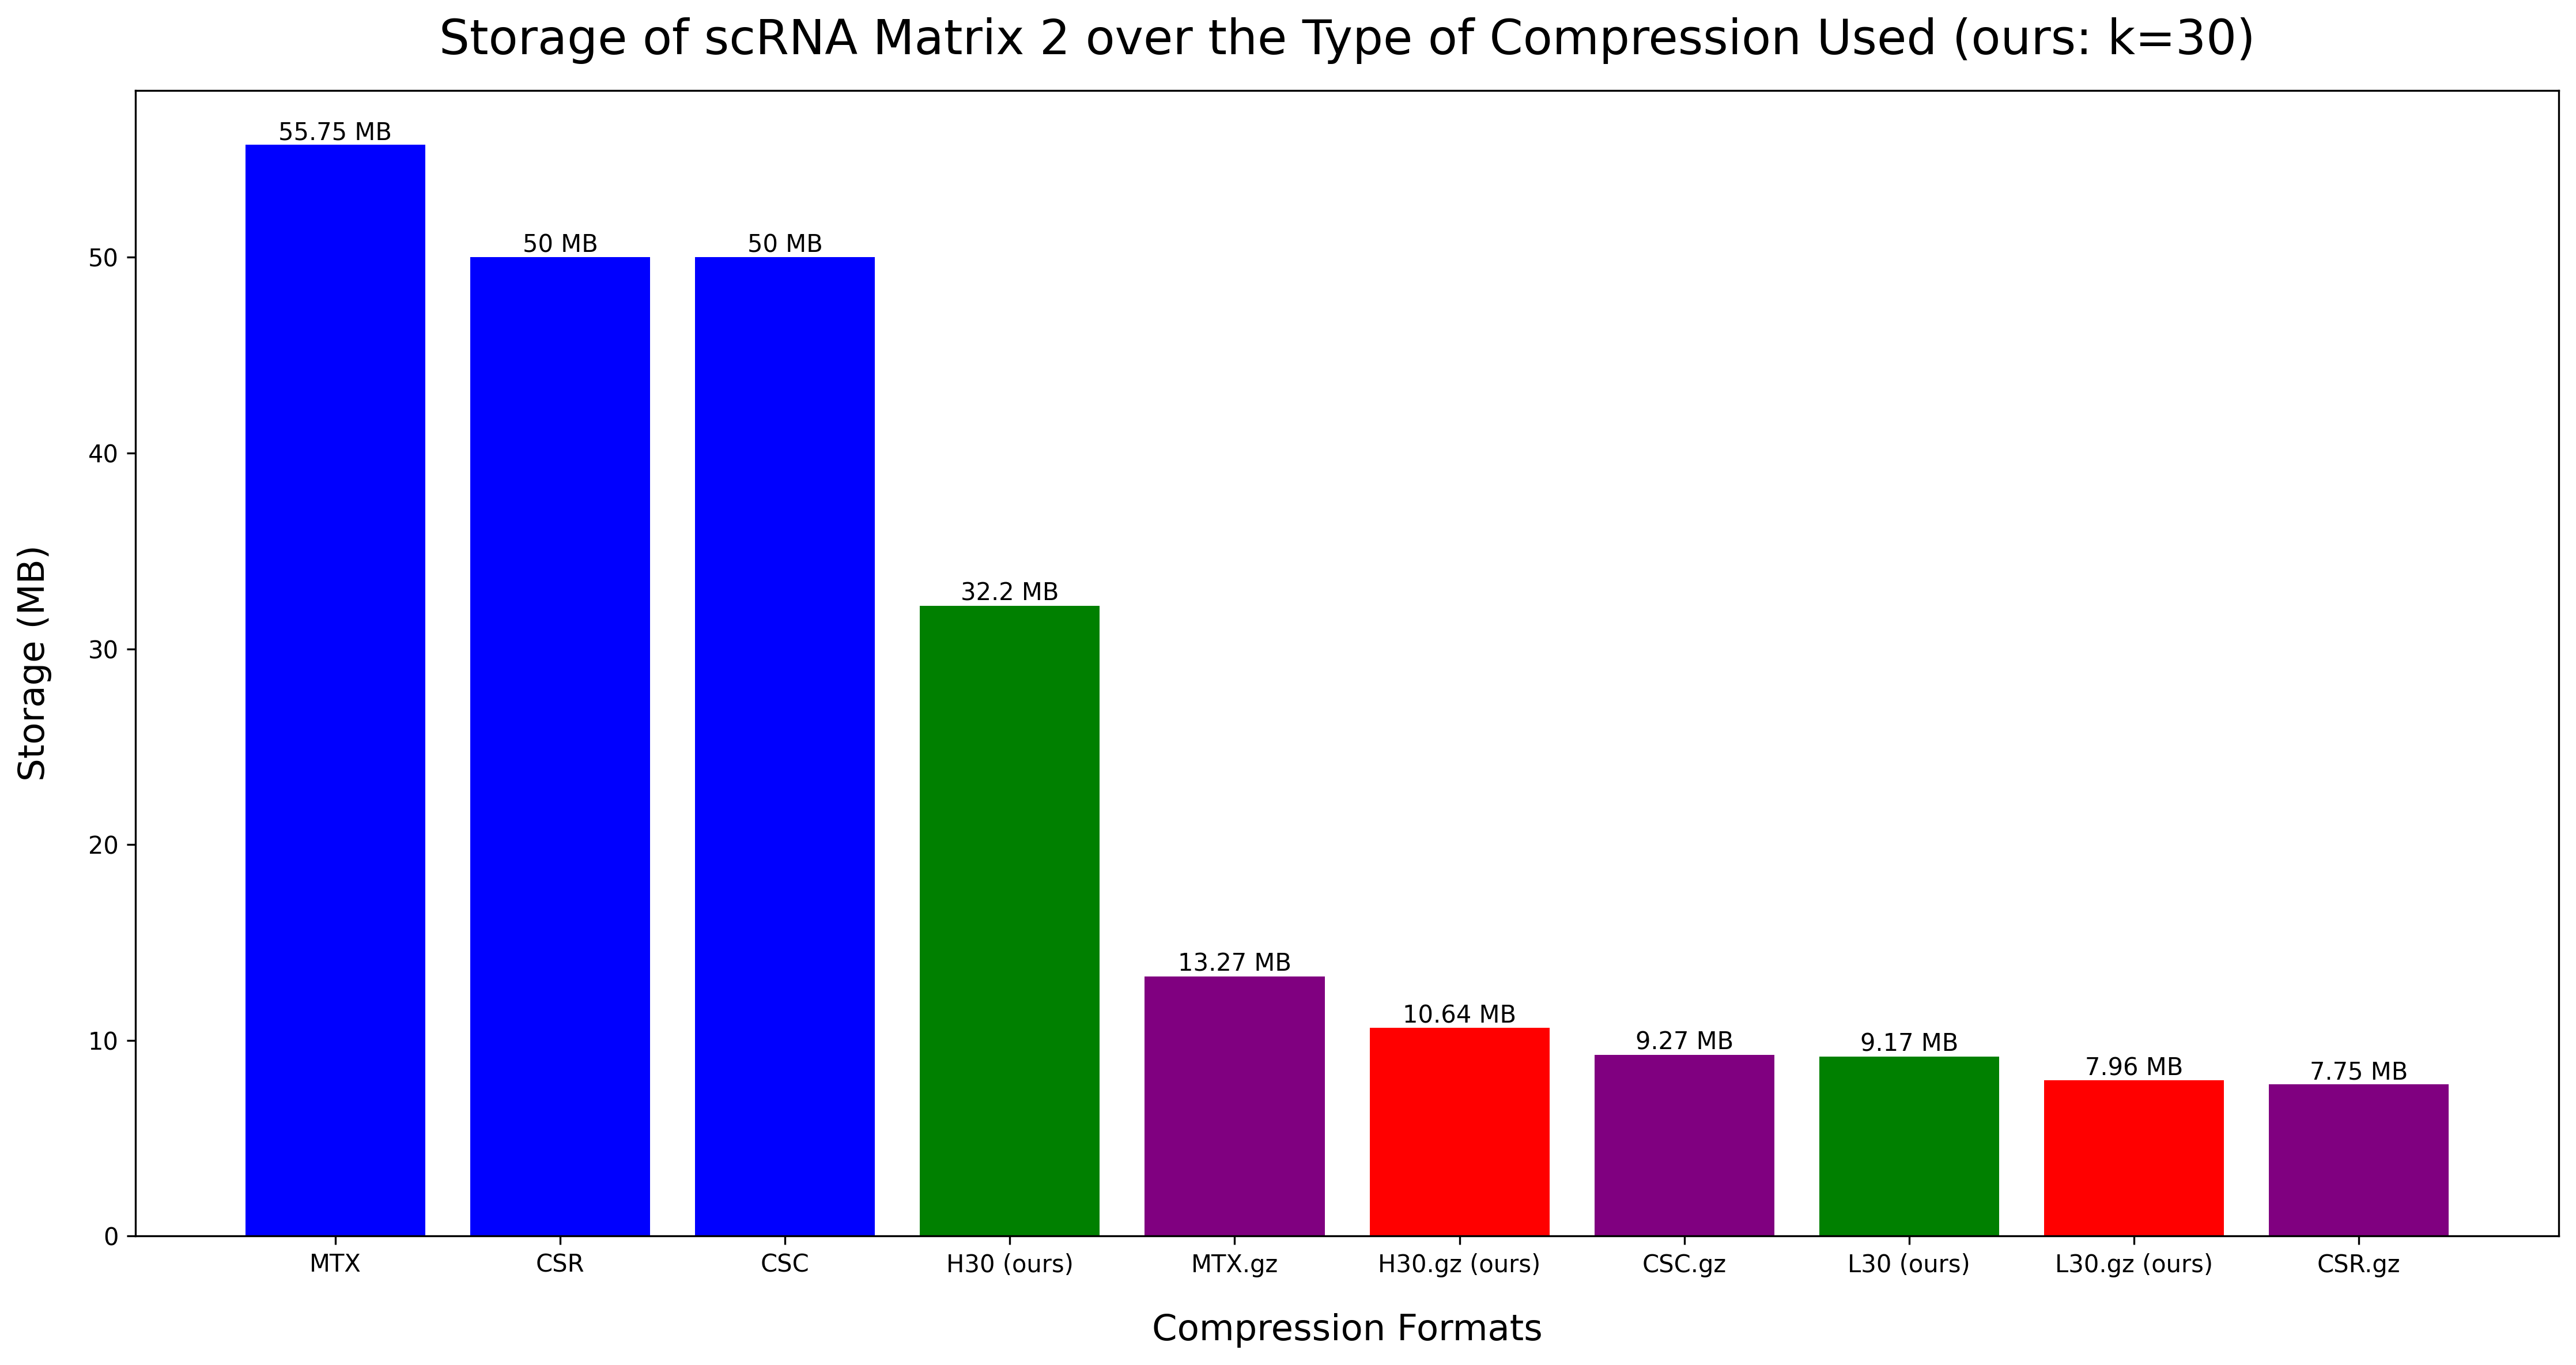
\includegraphics[width=0.35\textwidth]{compressed/kmeans/sample2/k30/storage_comparisons.png}\\
\textit{Comparison of storage sizes for different compression schemes on Sample 2 using $k$-means clustering with $k=30$.}

% Sample 1 neural, all k
\textbf{Figure S13. Sample 1, neural, $k=1$}:
\newline
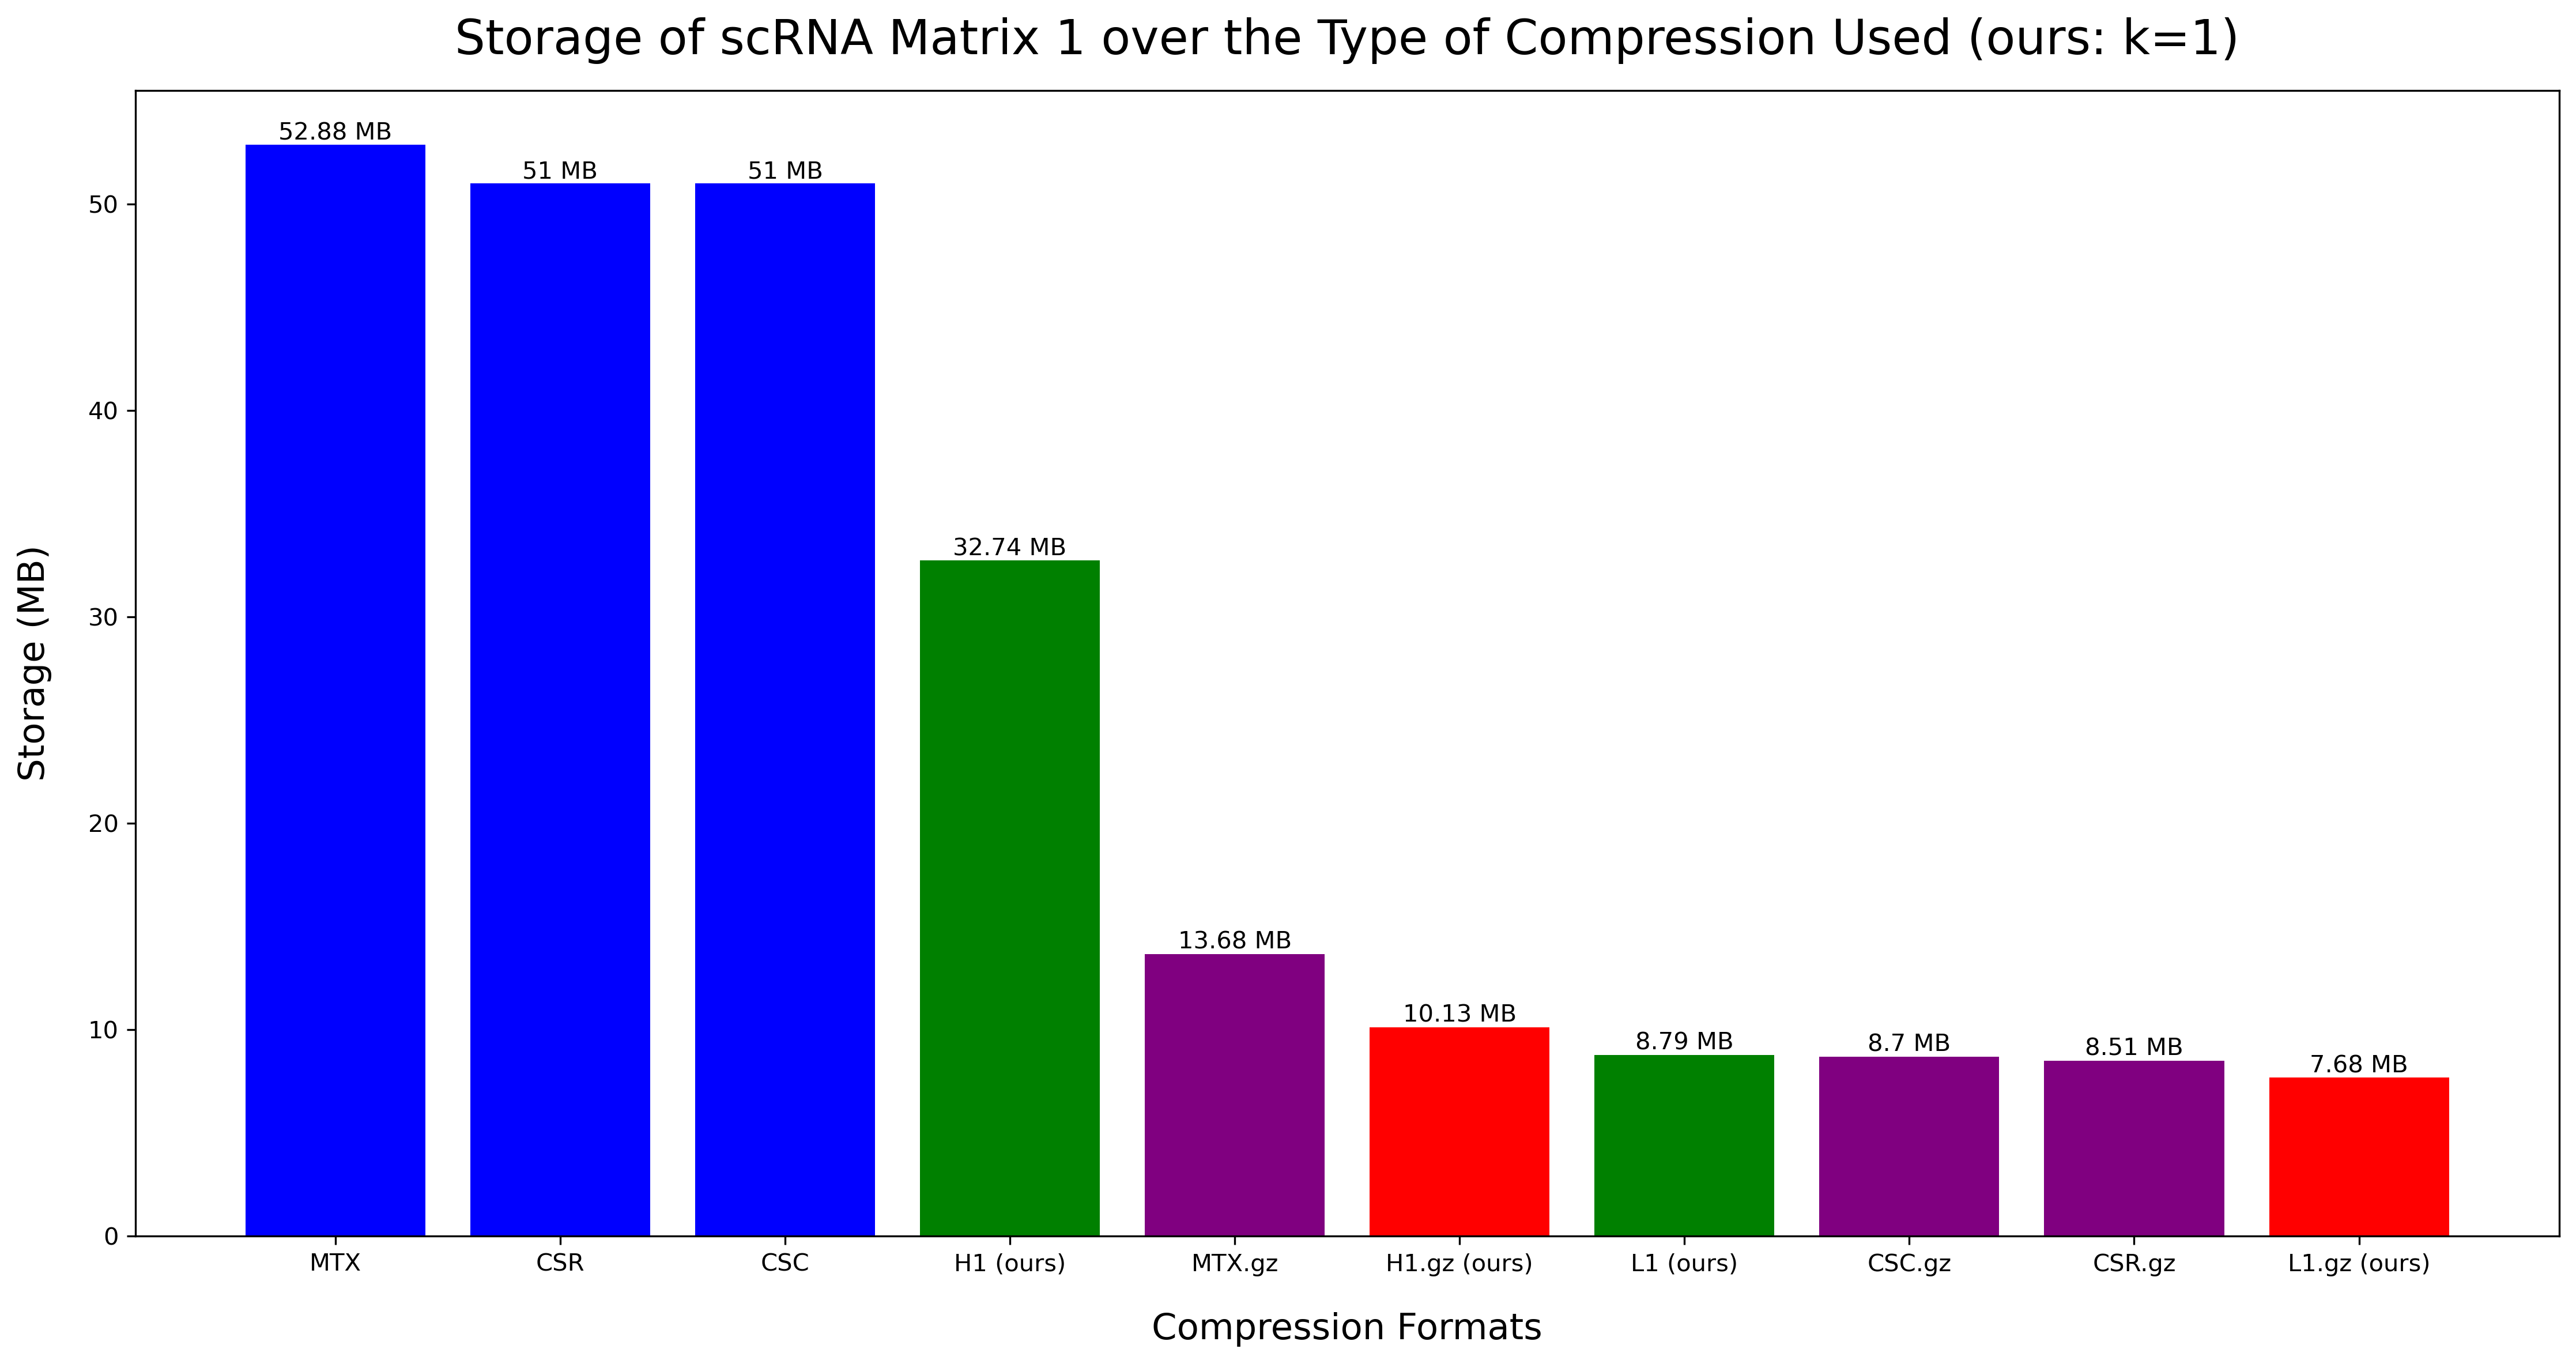
\includegraphics[width=0.24\textwidth]{compressed/neural/sample1/k1/storage_comparisons.png}
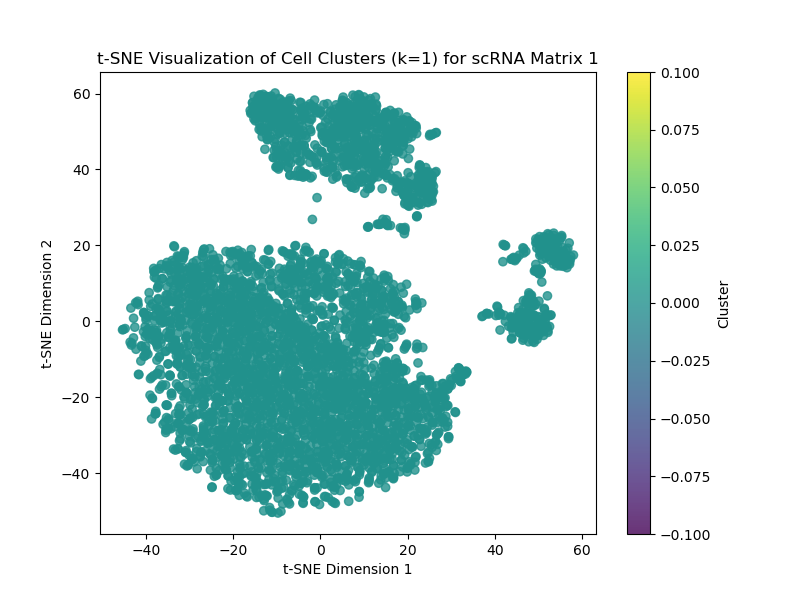
\includegraphics[width=0.24\textwidth]{compressed/neural/sample1/k1/clusters.png}\\
\textit{Left: Storage comparison for Sample 1 using neural clustering with $k=1$. Right: Cluster visualization for $k=1$.}

\textbf{Figure S14. Sample 1, neural, $k=2$}:
\newline
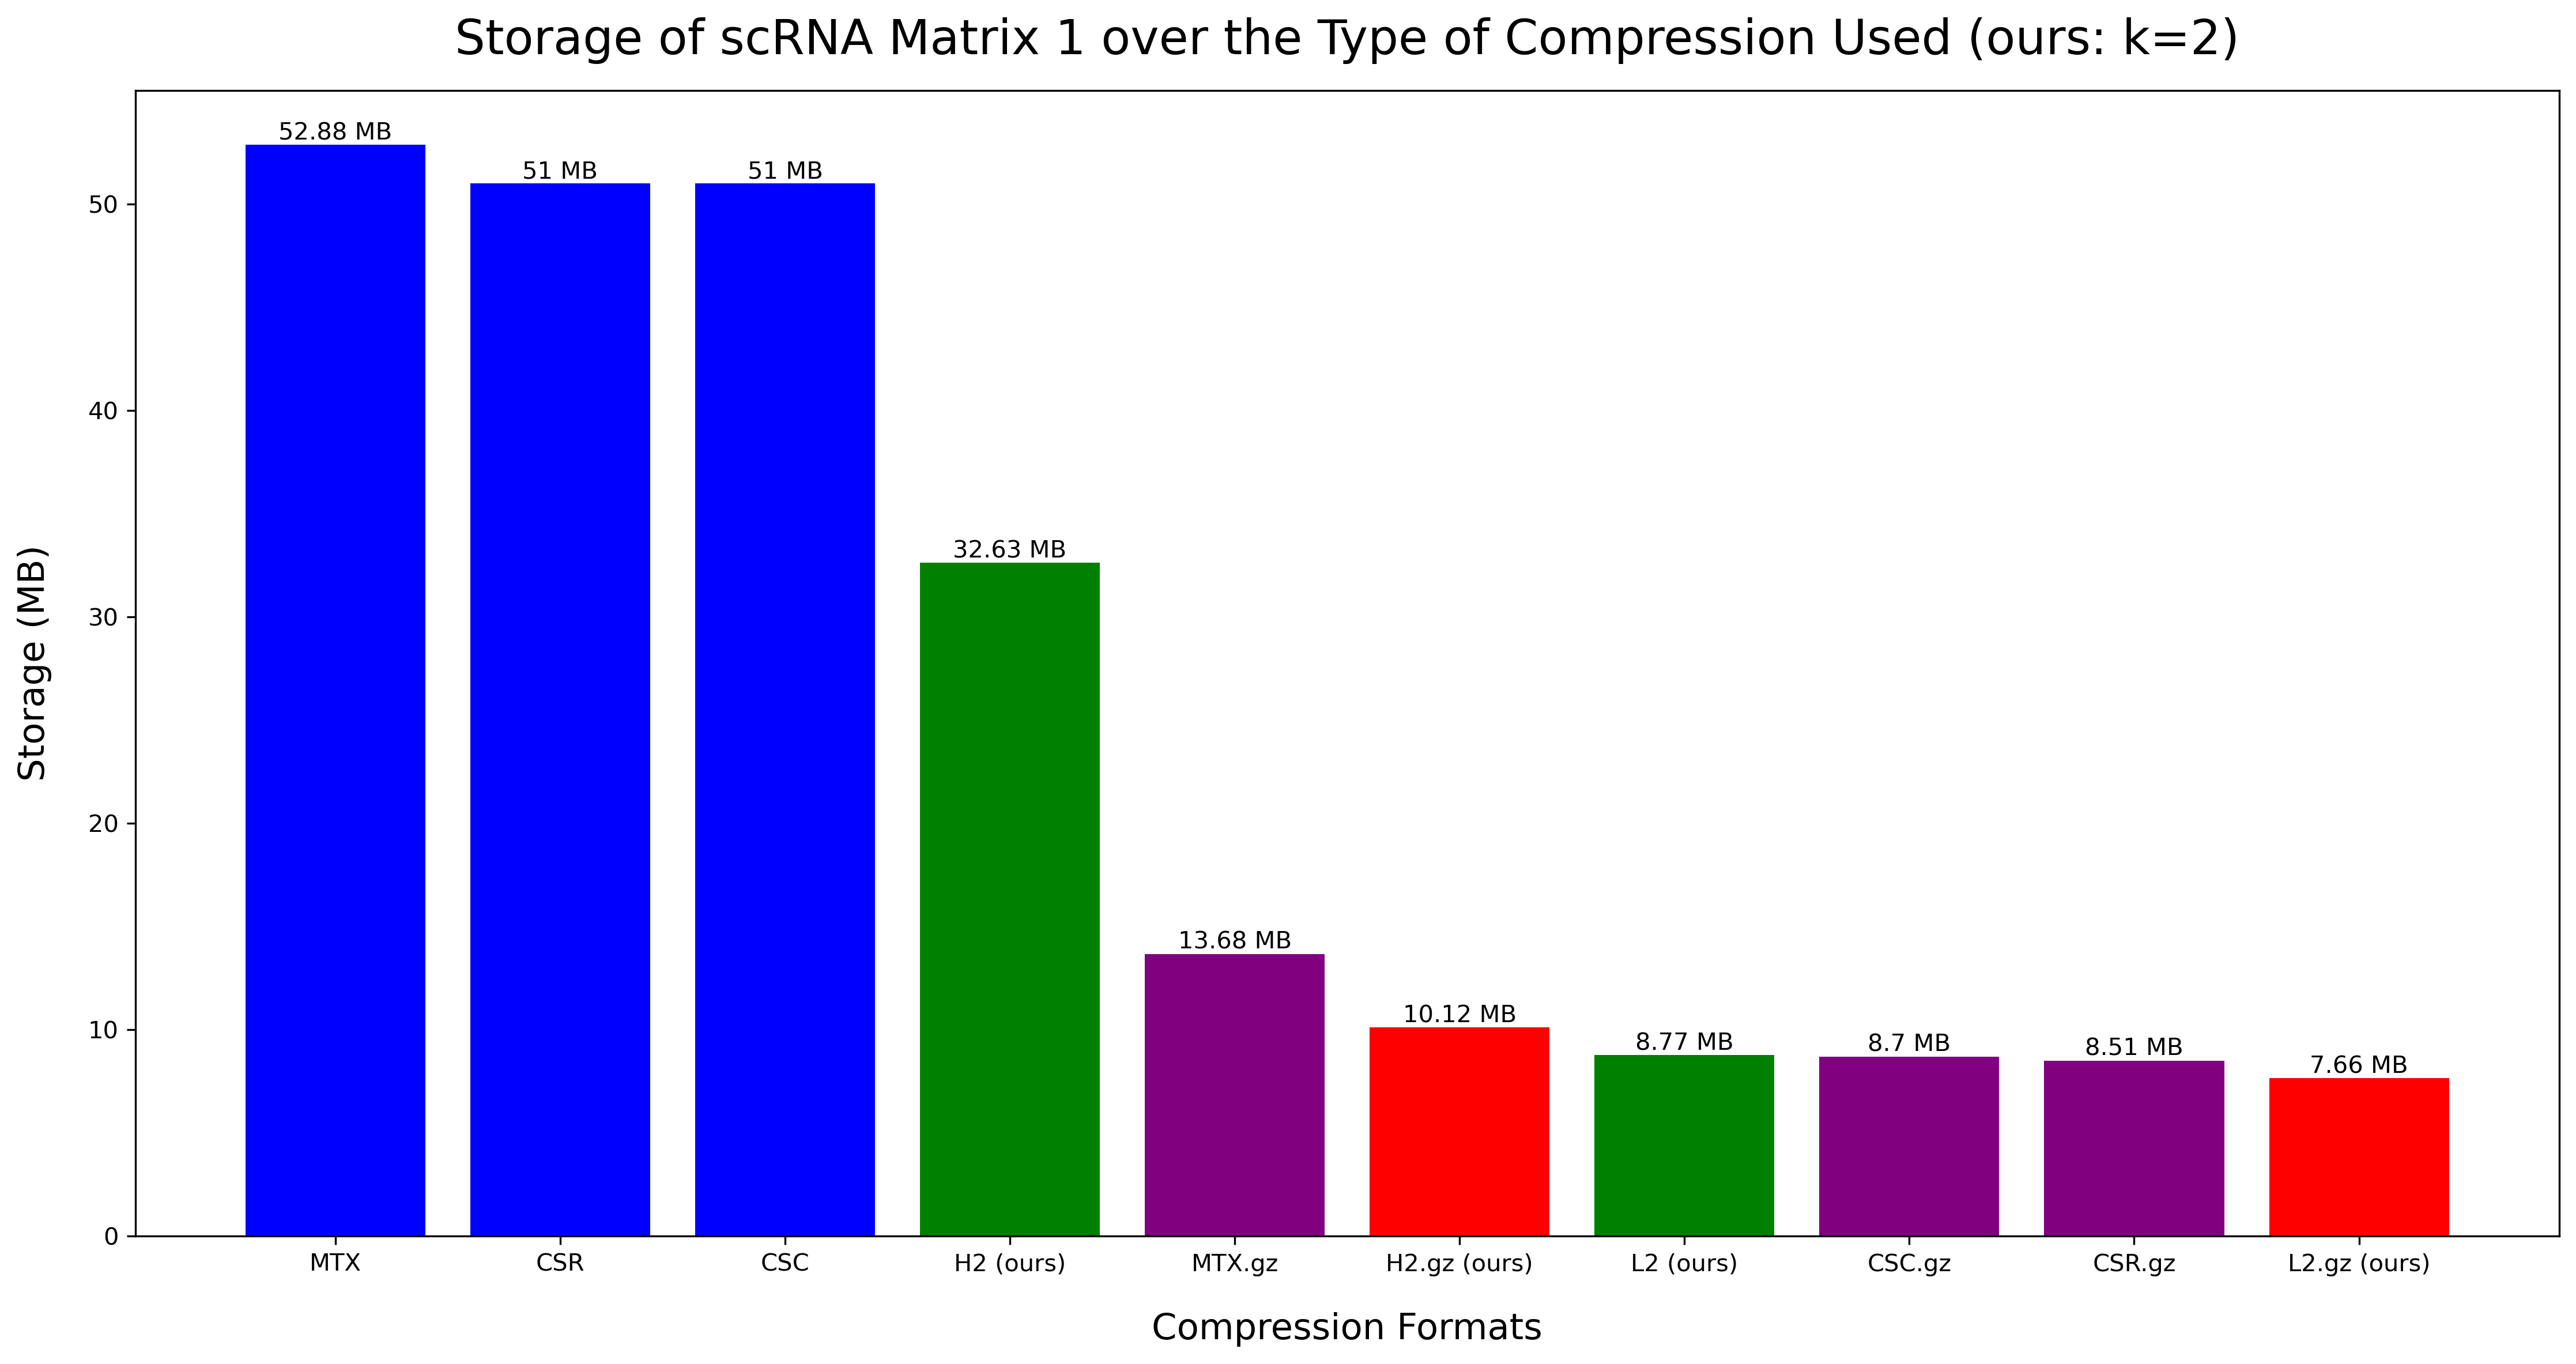
\includegraphics[width=0.24\textwidth]{compressed/neural/sample1/k2/storage_comparisons.png}
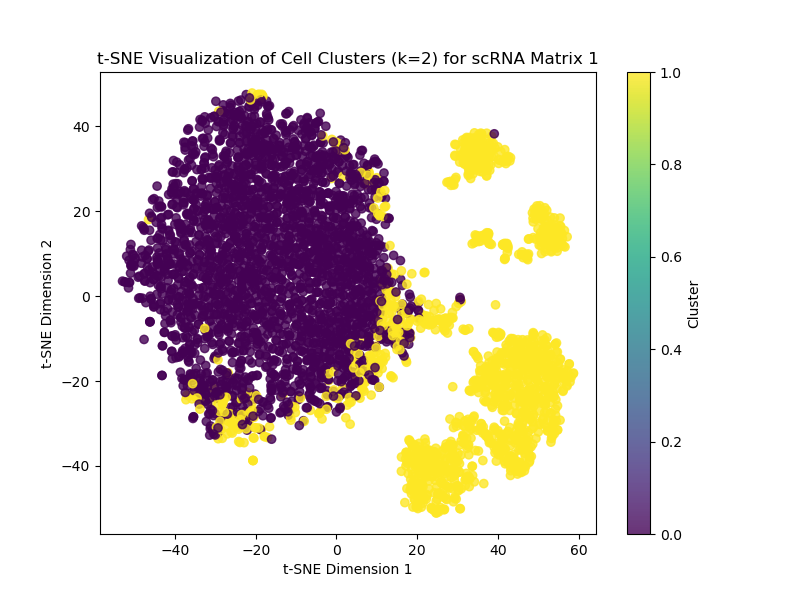
\includegraphics[width=0.24\textwidth]{compressed/neural/sample1/k2/clusters.png}\\
\textit{Left: Storage comparison for Sample 1 using neural clustering with $k=2$. Right: Cluster visualization for $k=2$.}

\textbf{Figure S15. Sample 1, neural, $k=5$}:
\newline
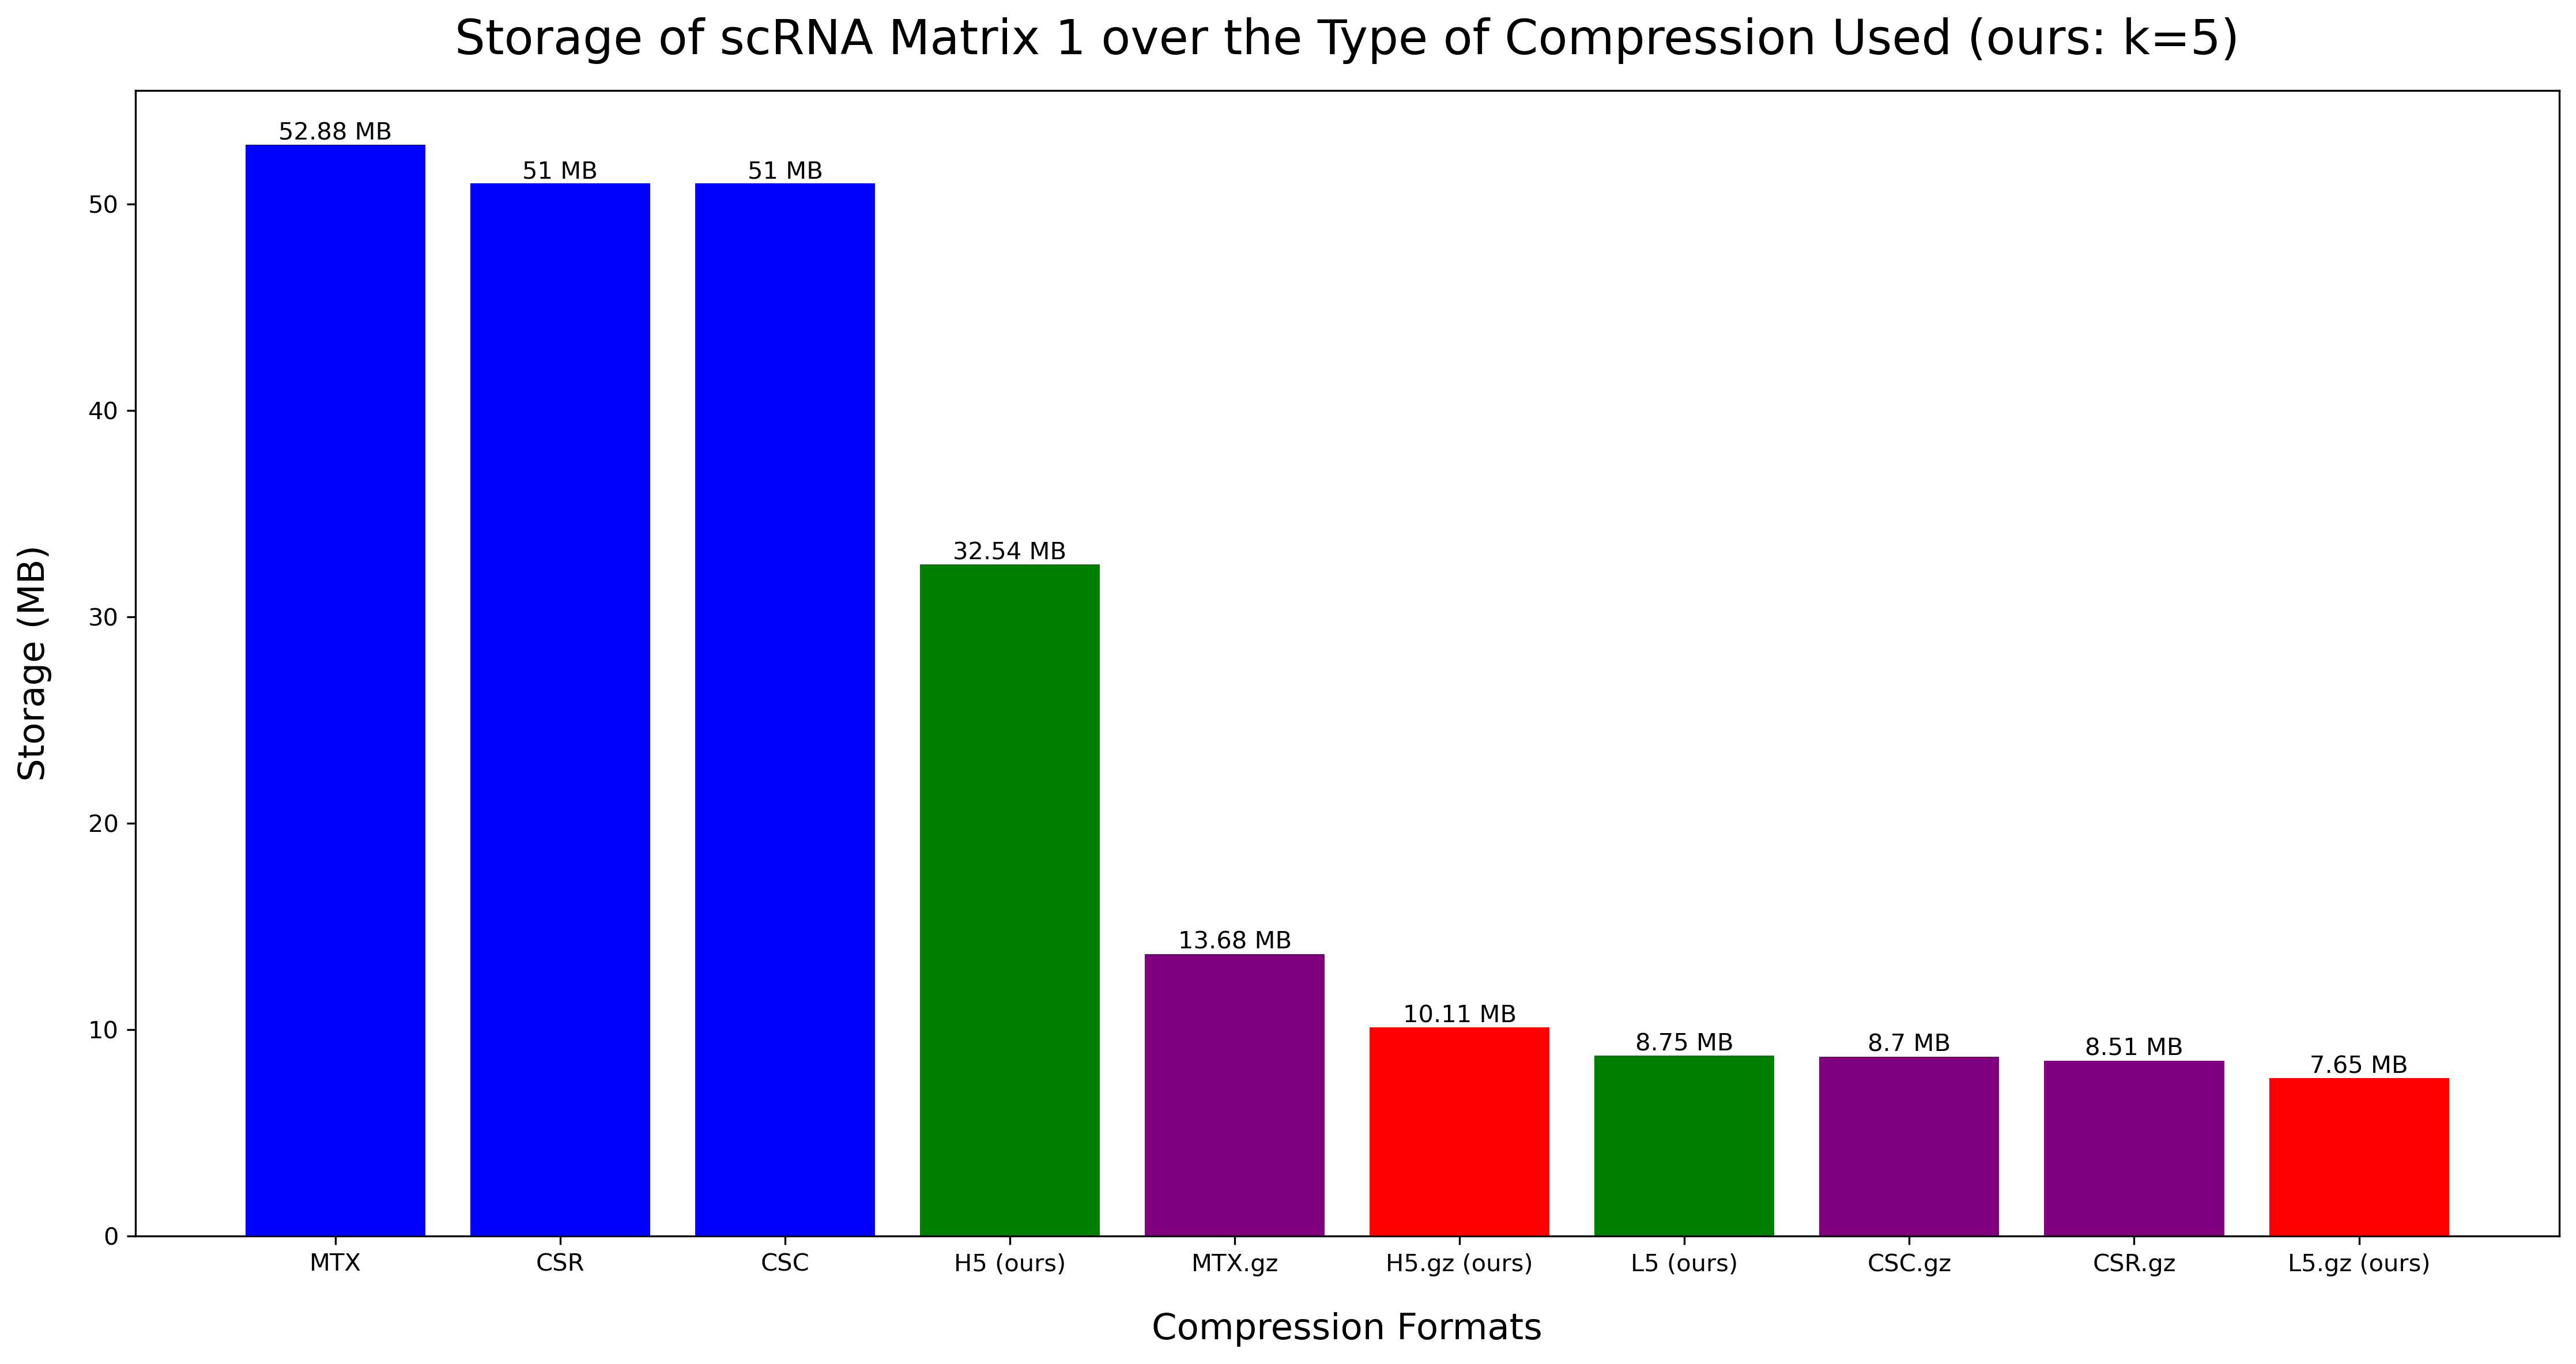
\includegraphics[width=0.24\textwidth]{compressed/neural/sample1/k5/storage_comparisons.png}
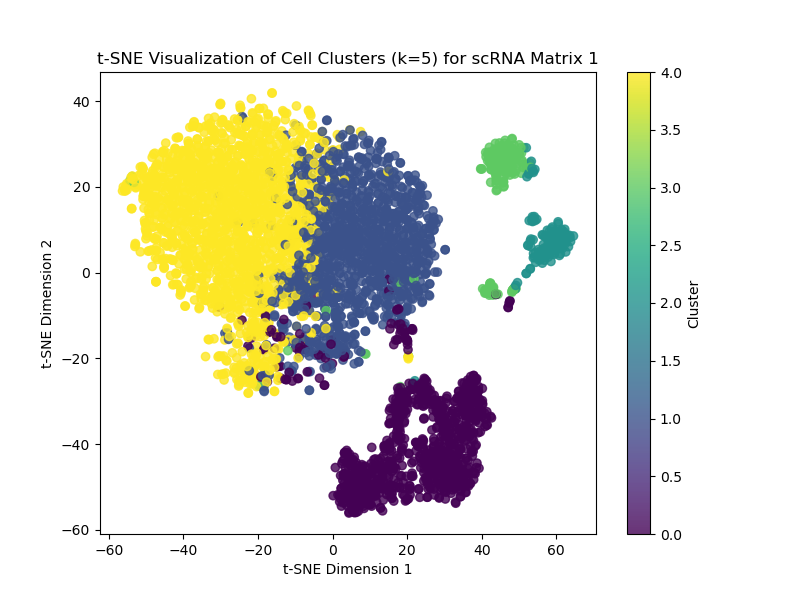
\includegraphics[width=0.24\textwidth]{compressed/neural/sample1/k5/clusters.png}\\
\textit{Left: Storage comparison for Sample 1 using neural clustering with $k=5$. Right: Cluster visualization for $k=5$.}

\textbf{Figure S16. Sample 1, neural, $k=10$}:
\newline
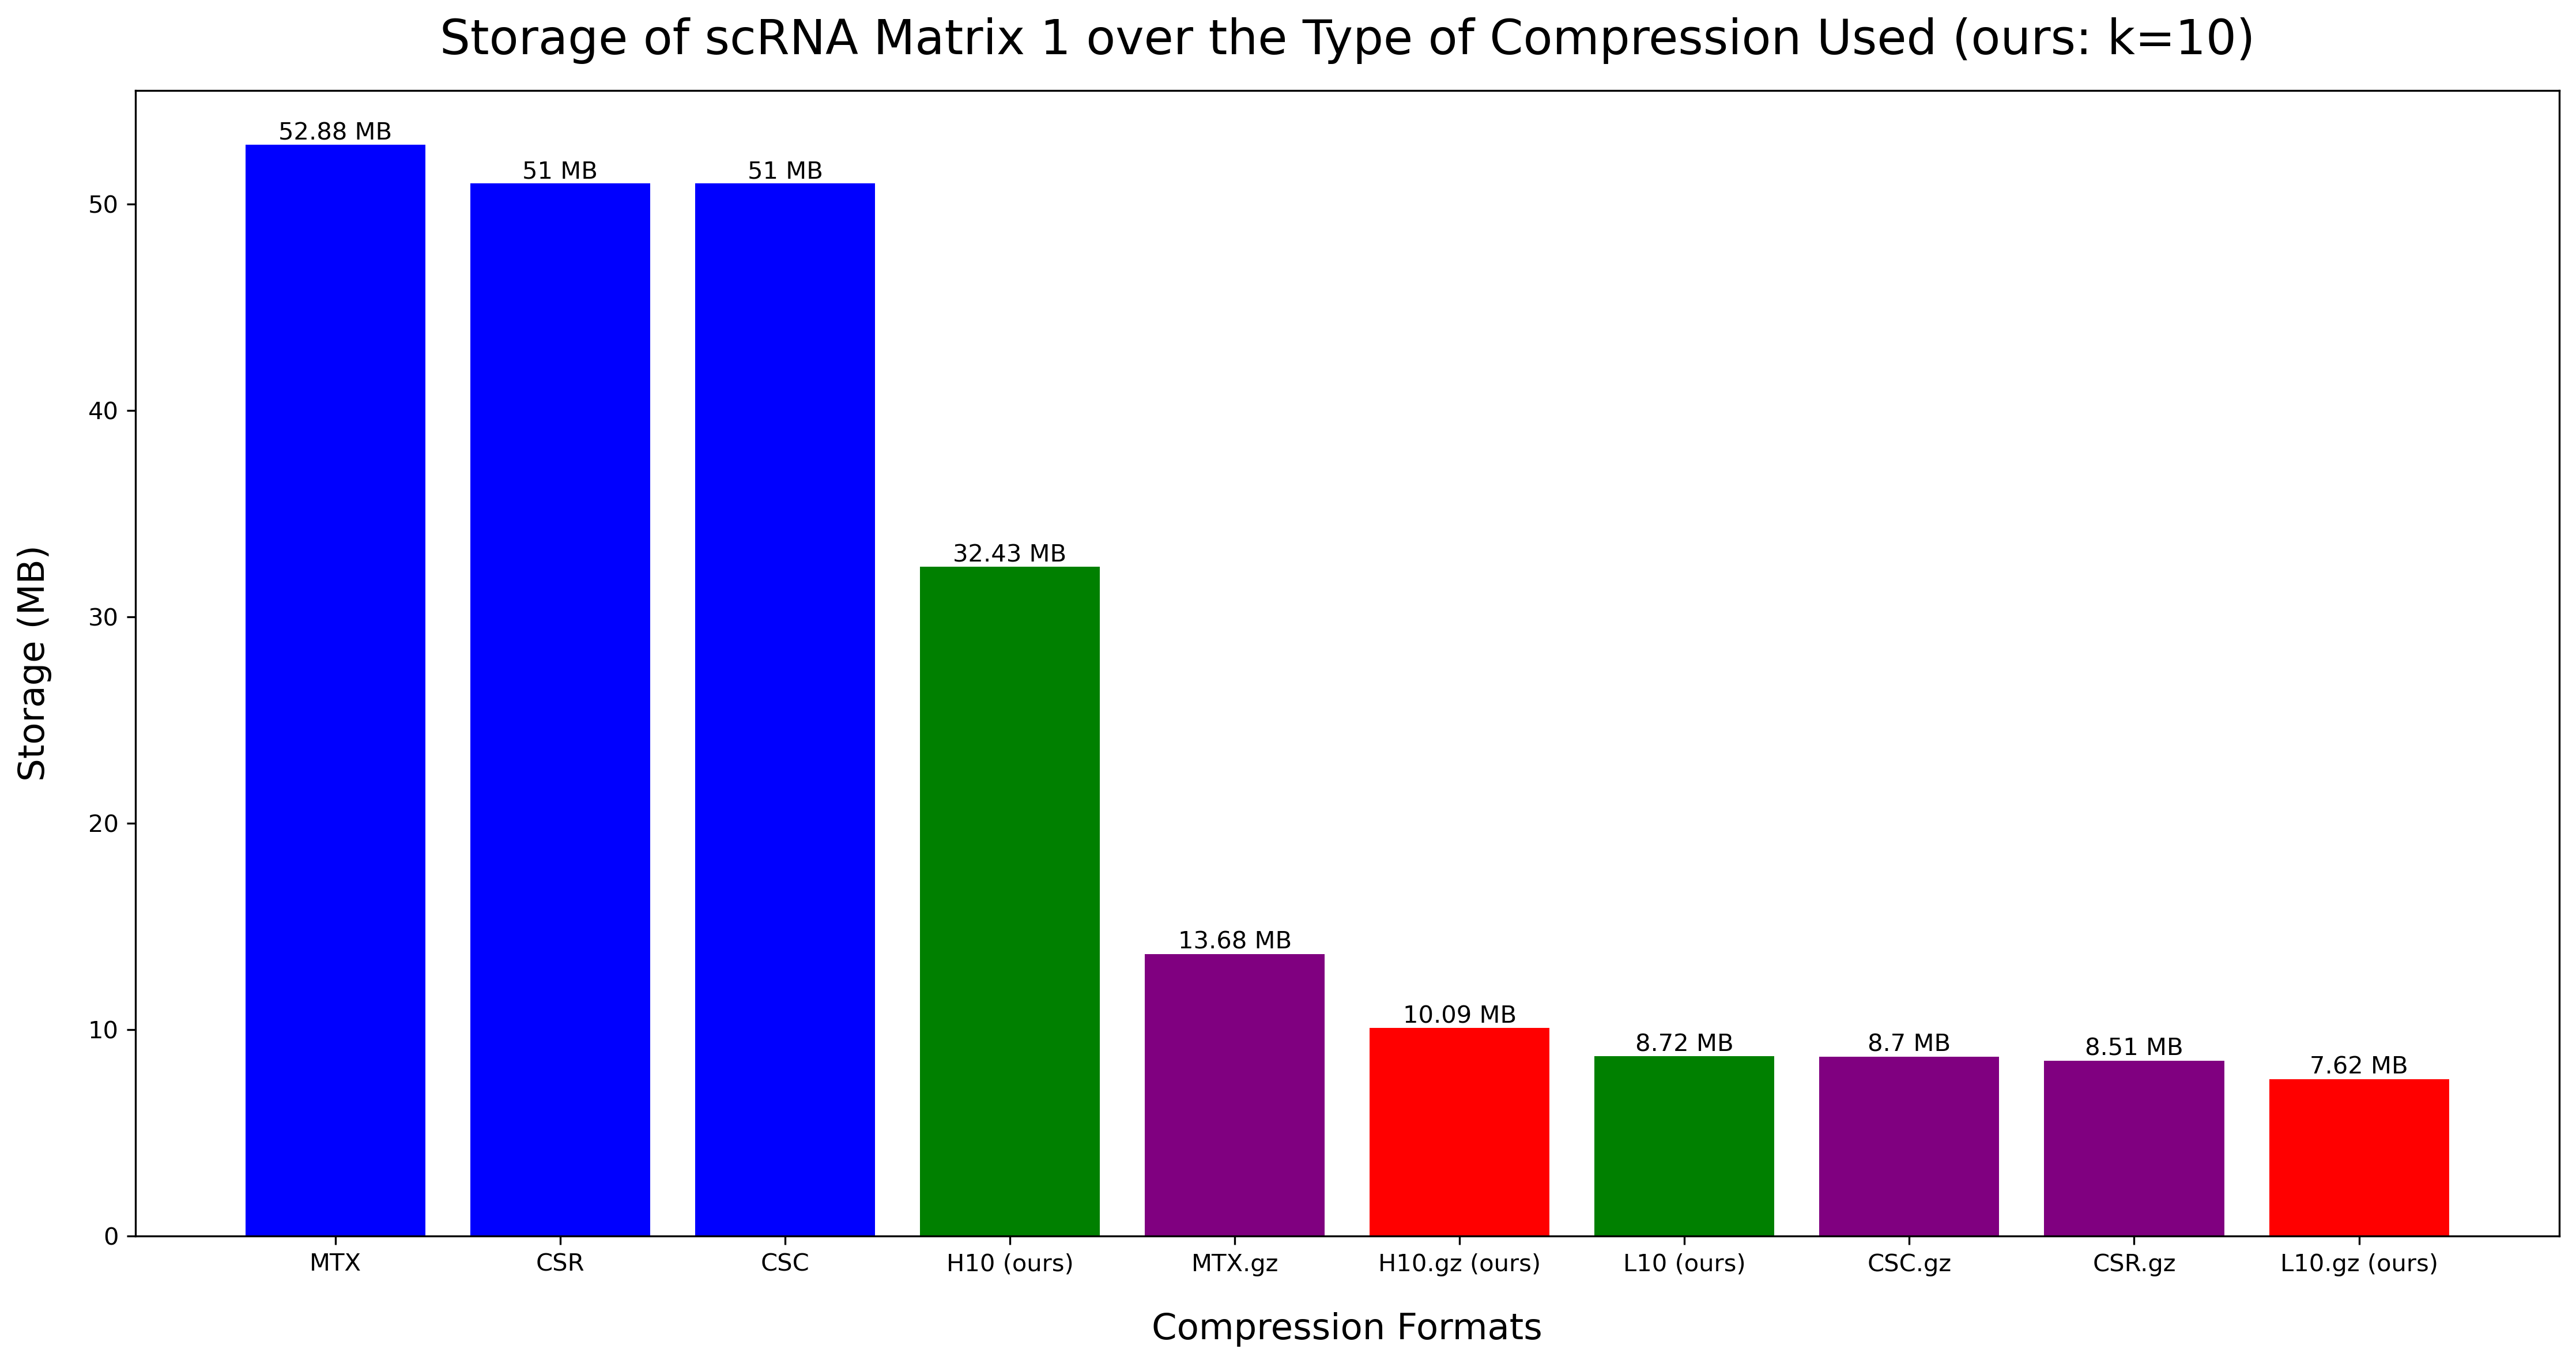
\includegraphics[width=0.24\textwidth]{compressed/neural/sample1/k10/storage_comparisons.png}
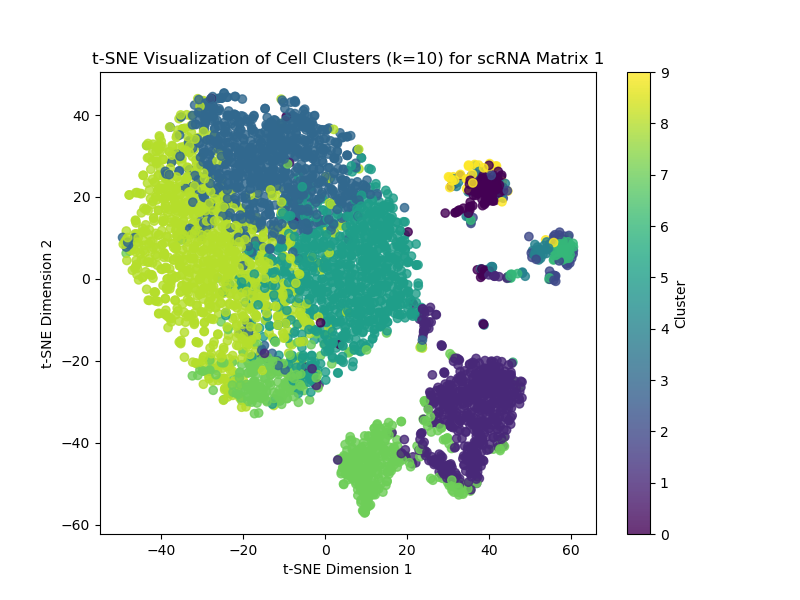
\includegraphics[width=0.24\textwidth]{compressed/neural/sample1/k10/clusters.png}\\
\textit{Left: Storage comparison for Sample 1 using neural clustering with $k=10$. Right: Cluster visualization for $k=10$.}

\textbf{Figure S17. Sample 1, neural, $k=20$}:
\newline
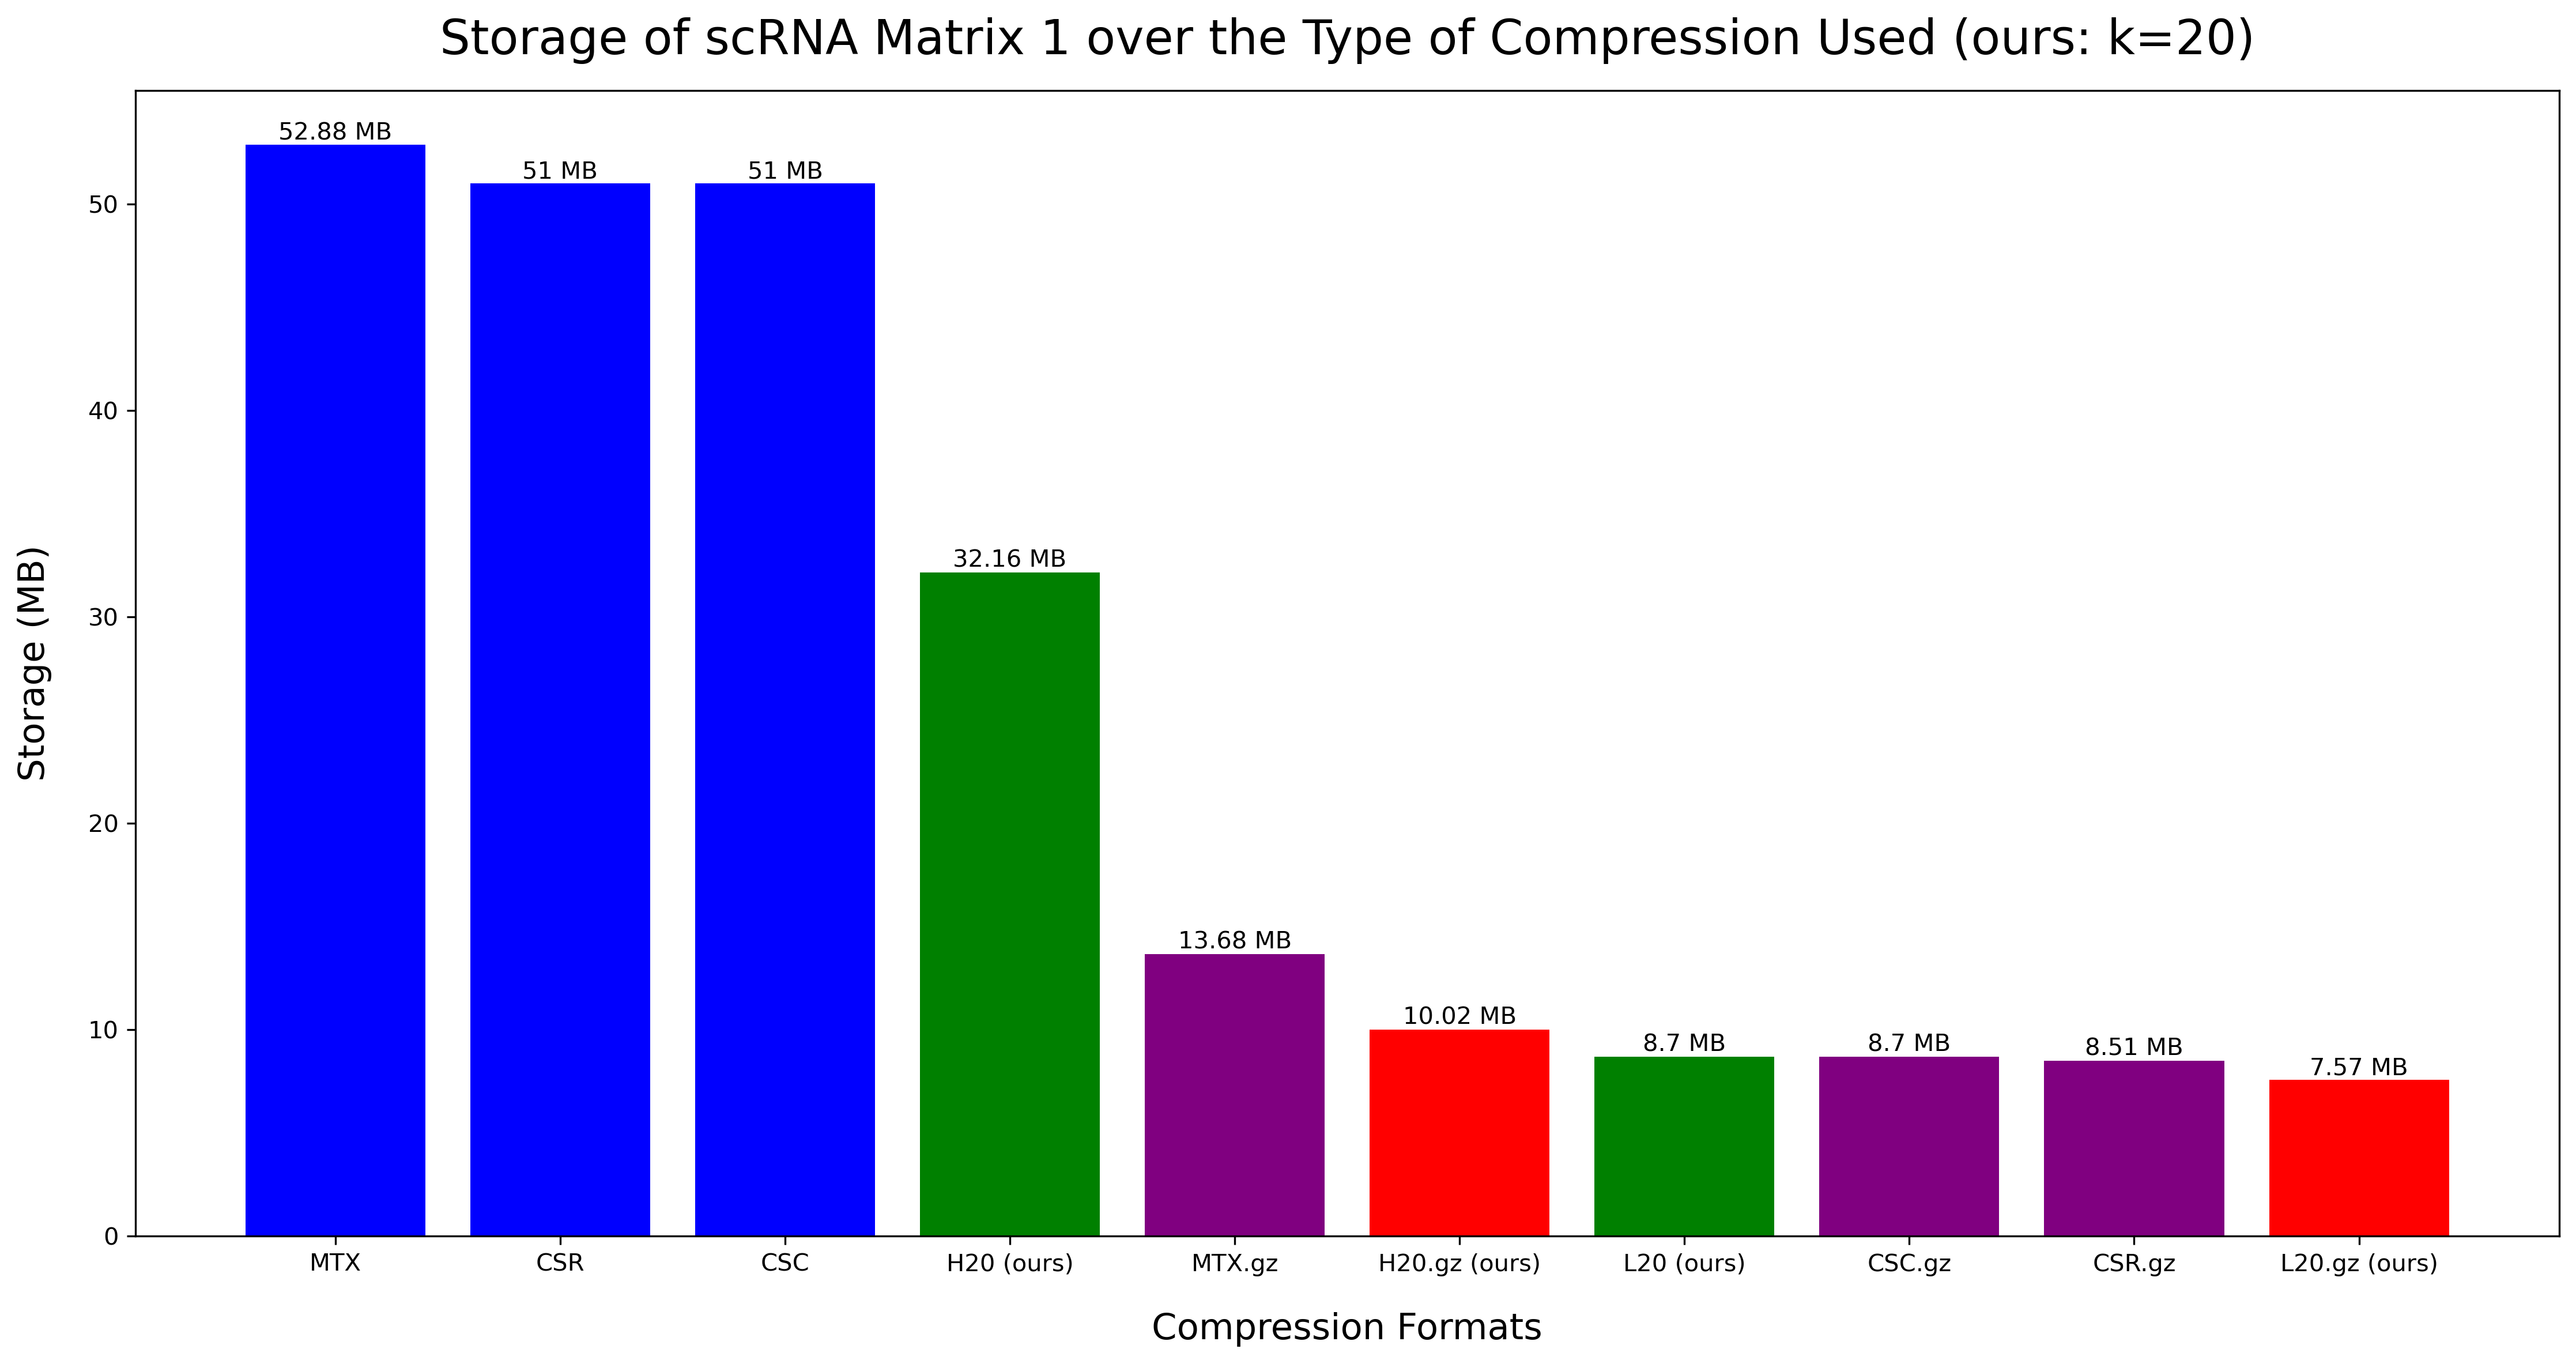
\includegraphics[width=0.24\textwidth]{compressed/neural/sample1/k20/storage_comparisons.png}
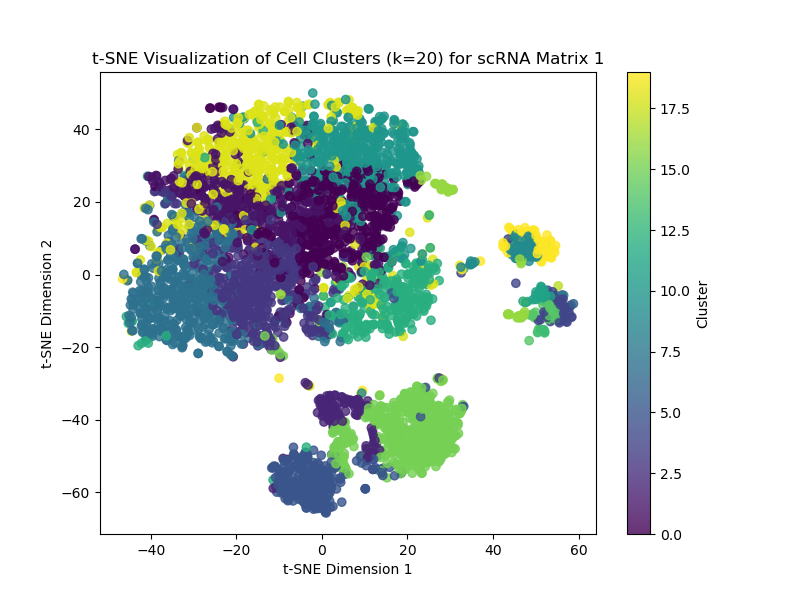
\includegraphics[width=0.24\textwidth]{compressed/neural/sample1/k20/clusters.png}\\
\textit{Left: Storage comparison for Sample 1 using neural clustering with $k=20$. Right: Cluster visualization for $k=20$.}

\textbf{Figure S18. Sample 1, neural, $k=30$}:
\newline
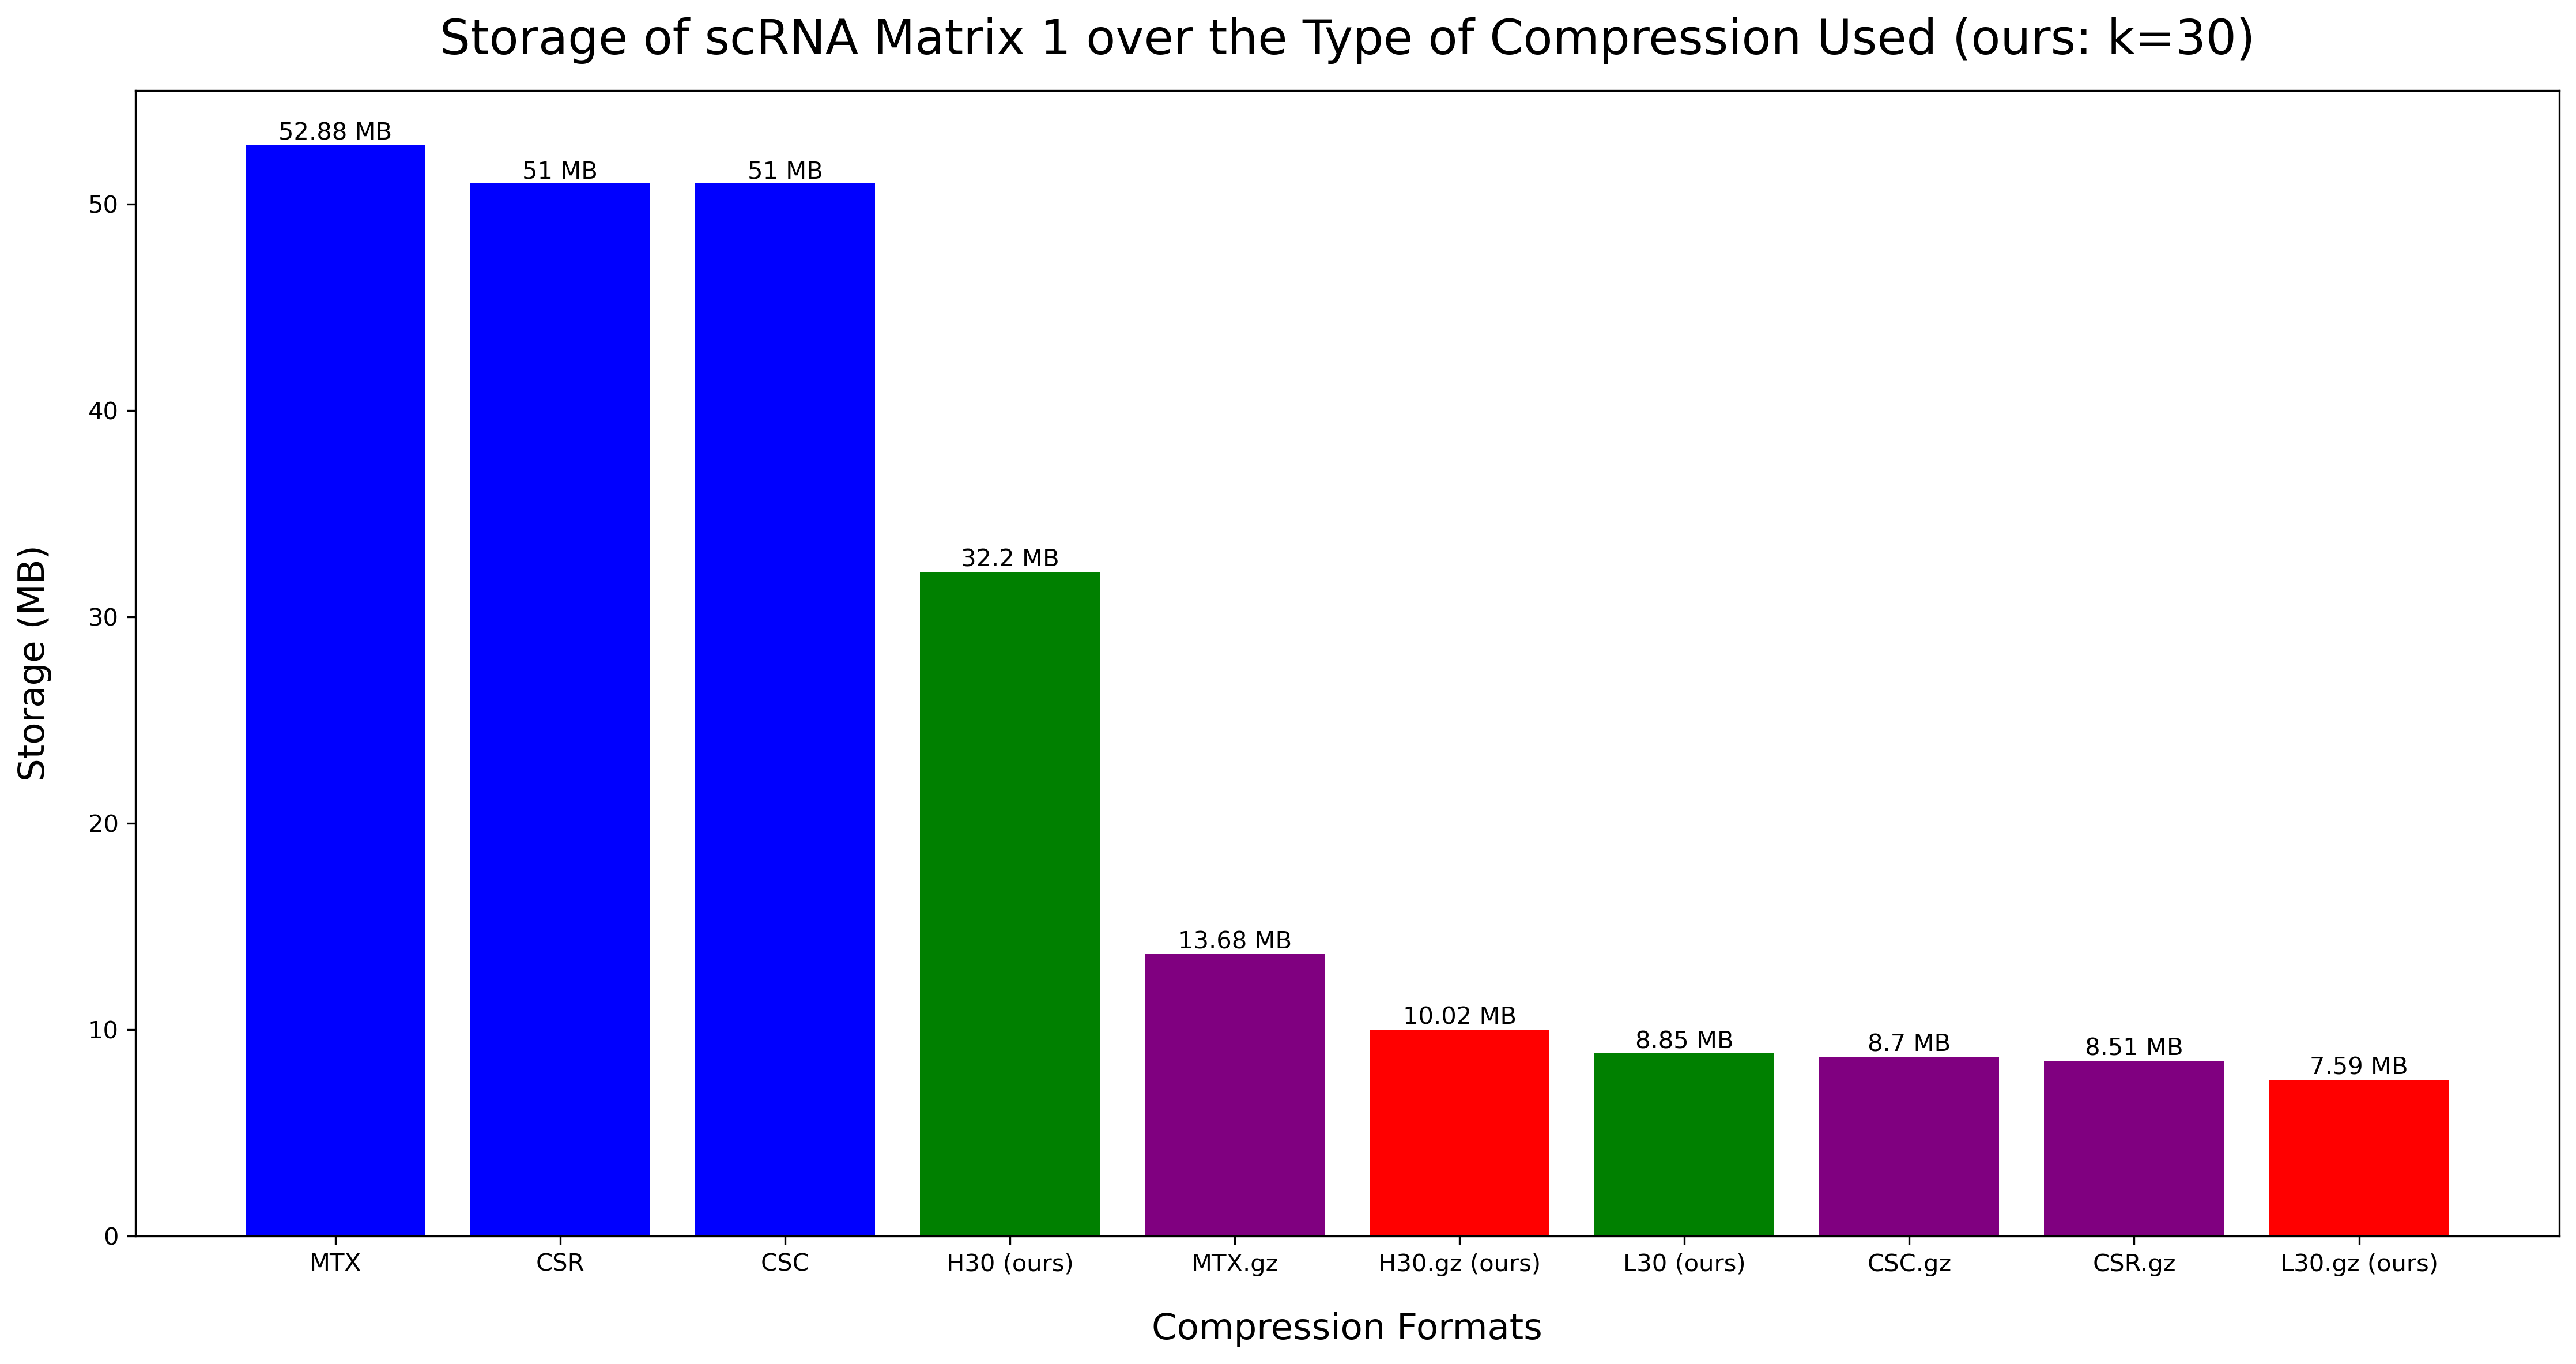
\includegraphics[width=0.24\textwidth]{compressed/neural/sample1/k30/storage_comparisons.png}
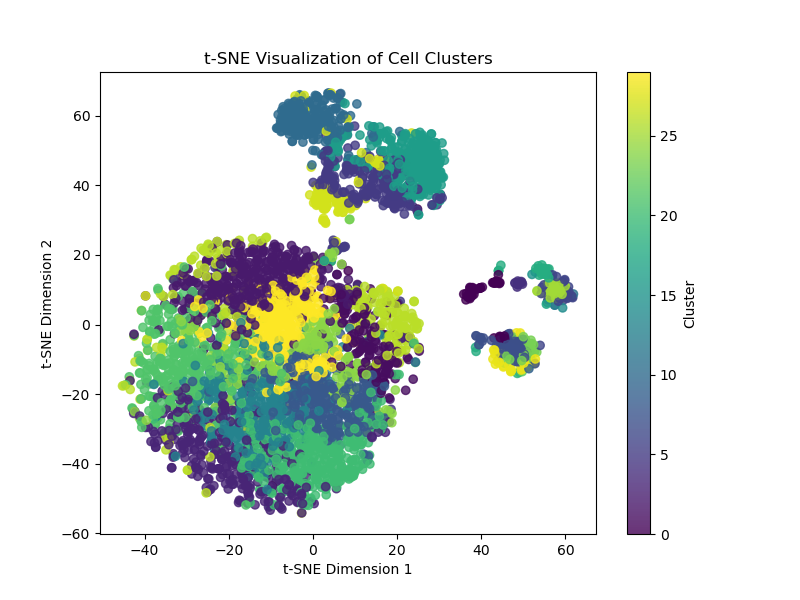
\includegraphics[width=0.24\textwidth]{compressed/neural/sample1/k30/clusters.png}\\
\textit{Left: Storage comparison for Sample 1 using neural clustering with $k=30$. Right: Cluster visualization for $k=30$.}

% Sample 2 neural, only k=30
\textbf{Figure S19. Sample 2, neural, $k=30$}:
\newline
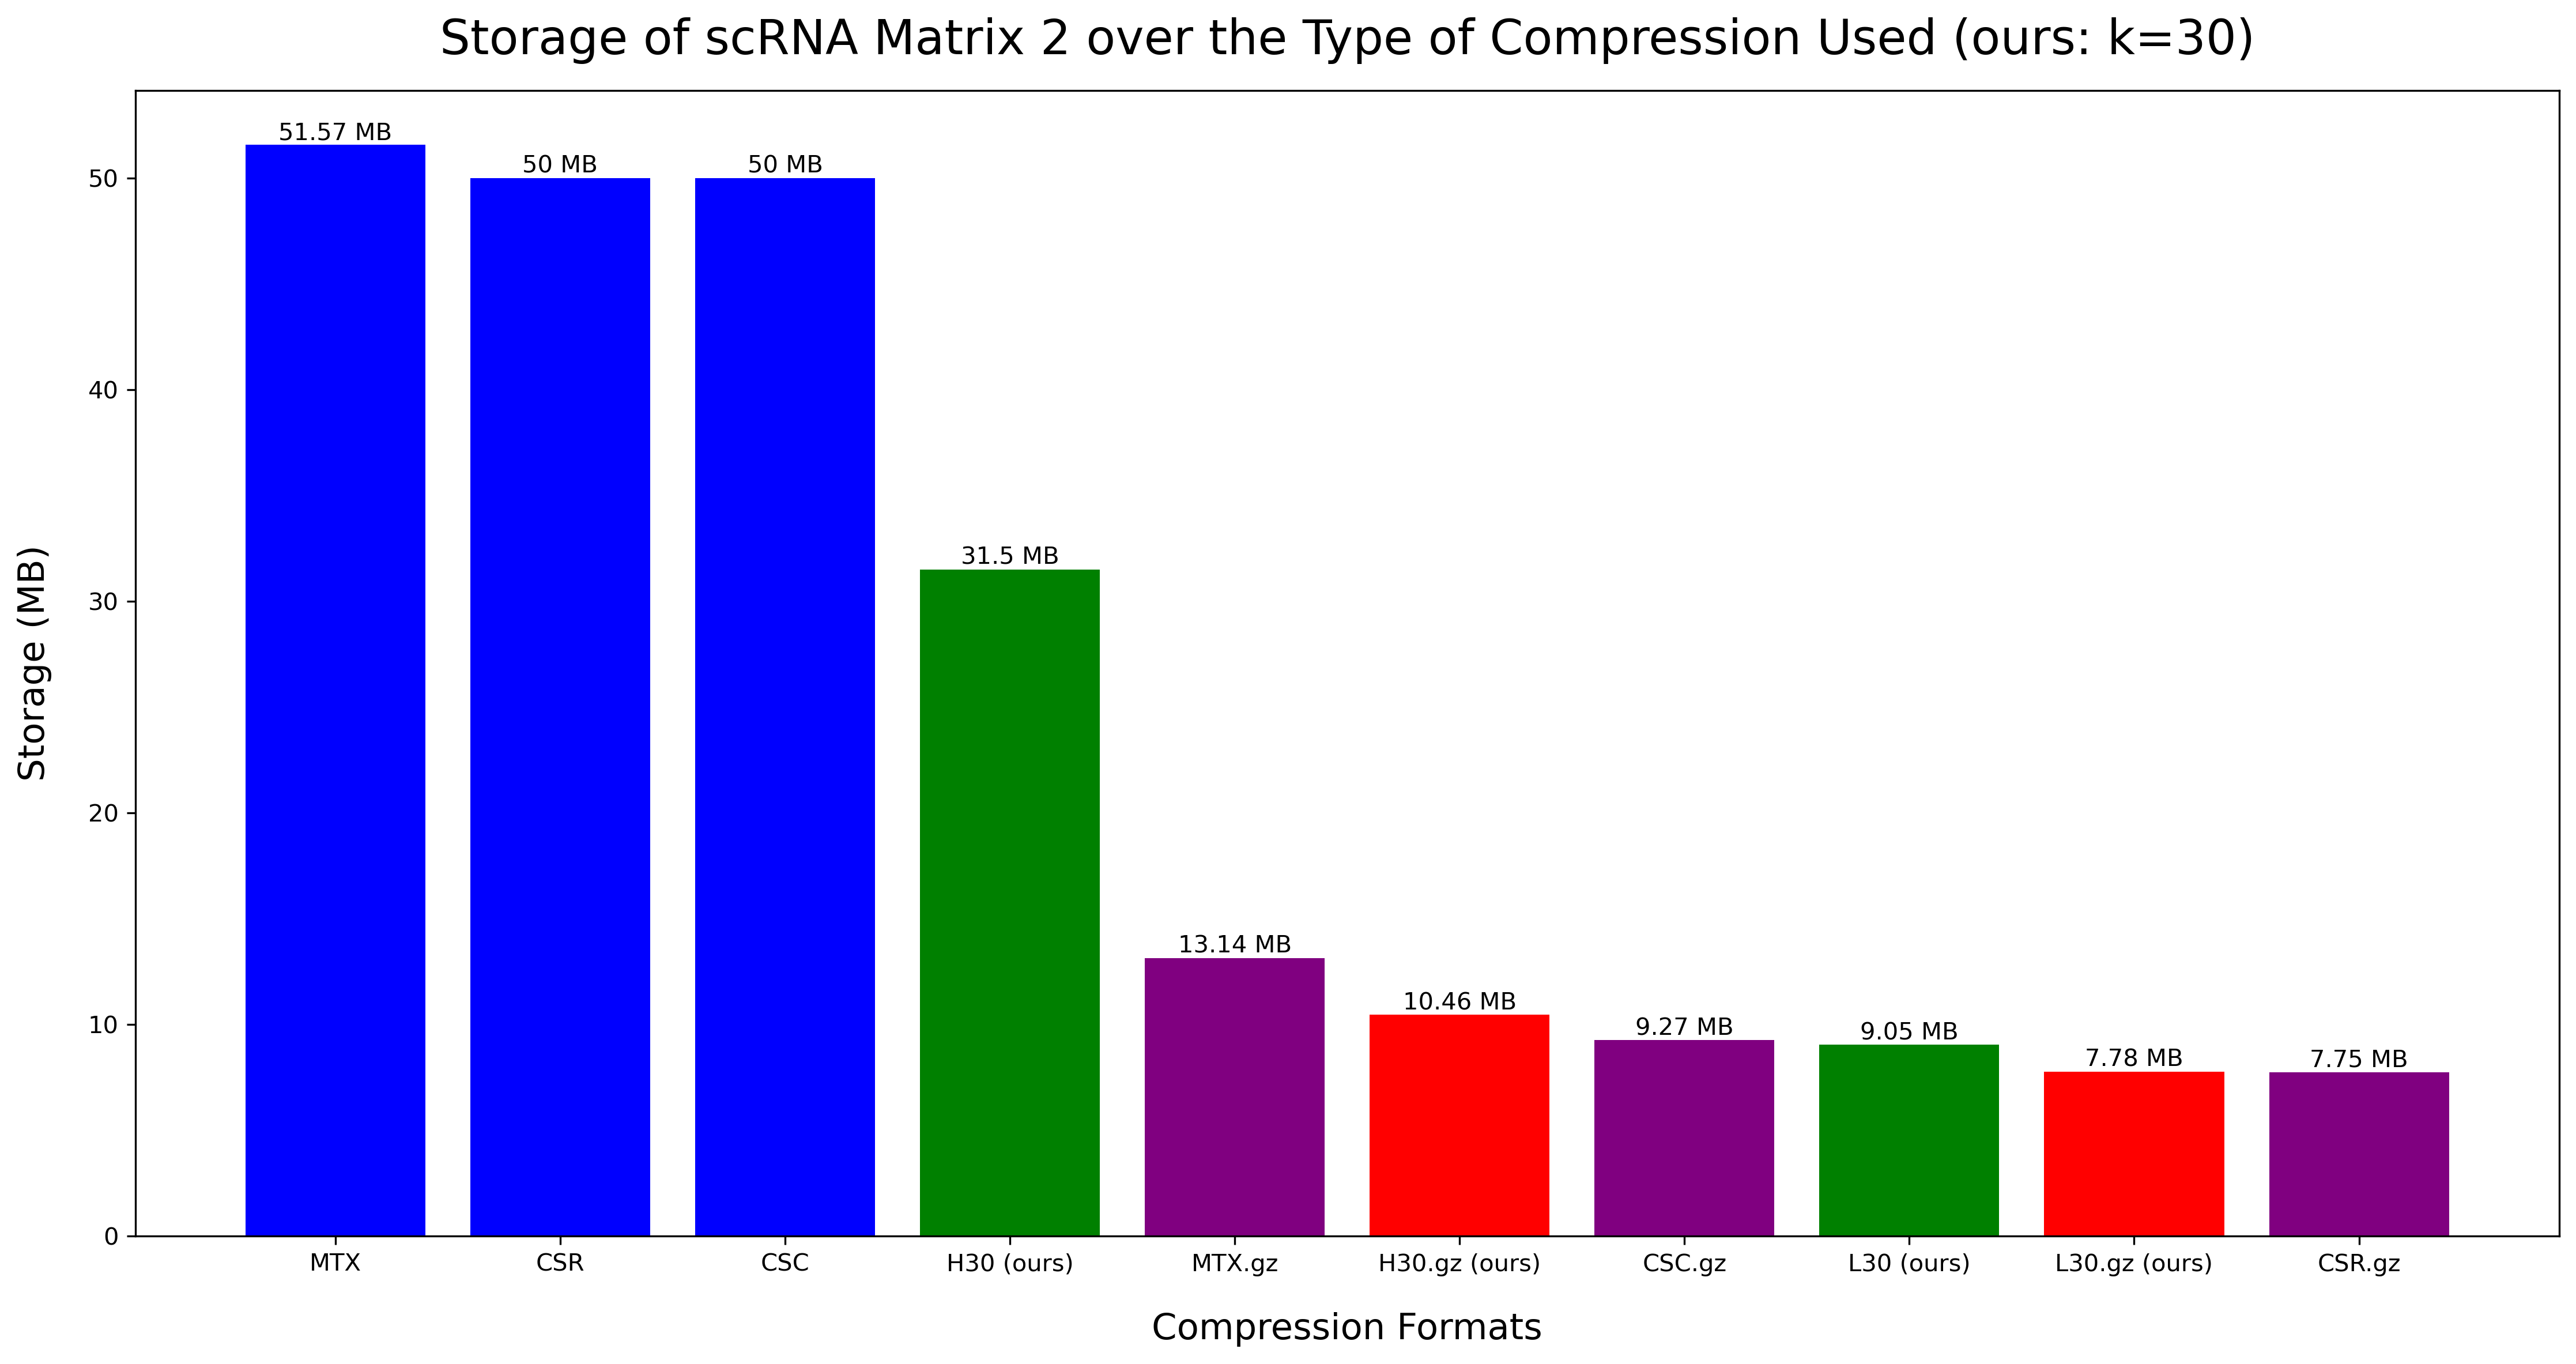
\includegraphics[width=0.24\textwidth]{compressed/neural/sample2/k30/storage_comparisons.png}
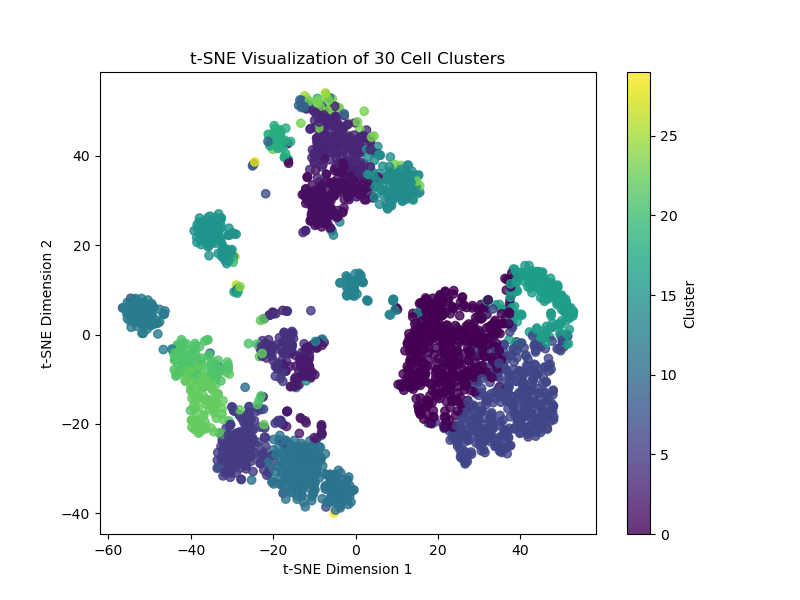
\includegraphics[width=0.24\textwidth]{compressed/neural/sample2/k30/clusters.png}\\
\textit{Left: Storage comparison for Sample 2 using neural clustering with $k=30$. Right: Cluster visualization for $k=30$.}

\end{document}
